\documentclass[11pt,UTF8]{ctexart}
\usepackage{geometry}
\usepackage{setspace}
\usepackage{amsthm,amsmath,amsfonts,amssymb}%\because\therefore
\usepackage{mathtools}%underset
\usepackage{gensymb}
\usepackage{cancel}
\usepackage{extarrows}
\usepackage{enumerate}
\usepackage{url}
\usepackage[unicode=true,%本行非常重要 支持中文目录hyperref CJKbookmarks对二级目录没用
	colorlinks,
	linkcolor=black,
	anchorcolor=black,
	citecolor=black,
	CJKbookmarks=false]{hyperref}

\newtheorem{theorem}{定理}
\newtheorem{definition}{定义}
\newtheorem{example}{例}%*去除编号
\newtheorem*{analysis}{分析}
\newtheorem{corollary}{推论}
\newtheorem*{corollary_convex}{推论}
\newtheorem{exercise}{练习}
\geometry{top=20mm,bottom=20mm,left=20mm,right=20mm}
\pagestyle{plain}%删除页眉

\def\zz{\mathbb{Z}}
\def\rr{\mathbb{R}}
\def\diff{\,\mathrm{d}}
\def\mmid{\enspace\Big|\enspace}
\def\eps{\varepsilon}
\def\disp{\displaystyle}
\newcommand{\ssum}[1]{\displaystyle\sum_{n=1}^{\infty}#1}
\newcommand{\ssumz}[1]{\displaystyle\sum_{n=0}^{\infty}#1}
\newcommand{\ssumk}[1]{\displaystyle\sum_{k=1}^{\infty}#1}
\newcommand{\ssumkn}[1]{\displaystyle\sum_{k=1}^{n}#1}
\newcommand{\limtoinf}[1]{\displaystyle\lim_{n\to\infty}#1}
\newcommand{\intab}[3]{\displaystyle\int_{#1}^{#2}{#3}\,\diff x}
\newcommand{\intabu}[4]{\displaystyle\int_{#1}^{#2}{#3}\,\diff #4}
\newcommand{\inpro}[1]{\langle #1\rangle}
\newcommand{\lrp}[1]{\left(#1\right)}
\newcommand{\lra}[1]{\left|#1\right|}
\newcommand{\nums}[1]{\{#1\}}
\newcommand{\floor}[1]{\lfloor#1\rfloor}

\renewcommand{\thefootnote}{\fnsymbol{footnote}}

\title{数学分析笔记整理V3.0}
\author{陈鸿峥}
\date{{\builddatemonth\today} \footnote{\text{Build \builddate\today}}}%加了build

\begin{document}

\maketitle
\renewcommand{\thefootnote}{\arabic{footnote}}
\setcounter{footnote}{0}

\setcounter{tocdepth}{2}%设置深度
\tableofcontents
\bigskip\bigskip\bigskip

\par 本文是笔者对数学分析这门数学基础课内容的一些整理,基本涵盖基本数学分析的全部内容,但以列举重要定理、提供不同思考问题的角度、提供解题思路为主,故不能当作教科书学习使用. 如果是众人皆知的事实,本文将不会提及,请读者自行翻书. 本文将基本微积分的知识进行了融合,优化了章节安排,将相似的内容放在一起,也方便大家融会贯通、复习整理. 文中的例题基本出自《数学分析简明教程》,部分出自《吉米多维奇习题集》,大多过程比较简练,主要阐述解题的思想和方法. 笔者数学水平有限,文中难免出现疏漏,如有不妥之处还请读者指出.

% !TEX root = main.tex
% 填坑:可数无穷 不可数无穷 阿列夫
\section{实数系基本定理}
\label{sec:real_fundamental}
\par 实数系的基本性质作为实分析的入门,有着举足轻重的作用,深挖的话会发现很多有意思或者是反直觉的结论,但我们在这里仅仅做出一些定理的阐述和证明的思路,更多的内容等待以后再进行补充. 虽然本章涉及到的内容比较抽象,但是读者应该能够脑补出相应的情形,通过直观的认知来得到证明或证伪的思路,这对其中的证明题非常有益.
\subsection{实数连续性}
\par 实数连续性涉及到数系扩充的过程. 有理数之间存在空隙,因而数学家对其进行扩充,添加了无理数后变成实数系,而实数系竟然就弥补了之前有理数系的缺陷,变得稠密且连续,这是一个相当强的结论.
\begin{definition}[戴德金(Dedekind)连续性准则]
有大小顺序稠密的数系$S$,对于其任一分划$A|B$,$\exists$唯一$c\in S:\forall a\in A,b\in B:a\leq c\leq b$(即要么$A$有最大值,要么$B$有最小值),则称$S$连续.
\end{definition}
由此准则可以推出$\mathbb{Q}$不是连续的. 需要注意:
\begin{enumerate}
	\itemsep -3pt
	\item 分划的断点$c$不一定属于$S$(正因$c\notin S$,$\mathbb{Q}$不连续)
	\item 分划要保证\textbf{不空、不漏、不乱}
\end{enumerate}
\begin{theorem}[实数基本定理]
对$\mathbb{R}$的任一分划$A|B$,$\exists$唯一$r\in S:\forall a\in A,b\in B:a\leq r\leq b$
\end{theorem}
\par 注意实数基本定理的证明是将实数全部以小数的形式表示,通过不断添加小数位数的方法来逼近割点,并没有用到后面的任何定理,可以算是根基.
\begin{definition}[确界]
如果实数集合$A$有上界,且上界中有最小数$\beta$,则定义$A$的上确界为$\sup A:=\beta$;若$A$有下界,且下界中有最大数$\alpha$,则定义$A$的下确界为$\inf A:=\alpha$.
由定义可知,$\beta$为$A$上确界,当且仅当
\begin{enumerate}
	\itemsep -3pt
	\item $\forall x\in A:\,x\leq\beta$
	\item $\forall\varepsilon>0,\exists x_\varepsilon\in A:\,x_\varepsilon >\beta-\varepsilon$
\end{enumerate}
\par 类似地也有下确界的充要条件.
\begin{example}
若$f(x)$在$[a,b]$上有界,定义其振幅为
\[\omega_f[a,b]=\sup_{x\in[a,b]}f(x)-\inf_{x\in[a,b]}f(x)\]
则
\[\omega_f[a,b]=\sup_{x',x''\in[a,b]}|f(x')-f(x'')|\]
\end{example}
\begin{analysis}
设$\disp\sup_{x\in[a,b]}f(x)=M,\inf_{x\in[a,b]}f(x)=m$,由确界的定义有
\[\forall x',x''\in[a,b]:\,f(x')\leq M,f(x'')\geq m\]
故$f(x')-f(x'')\leq M-m$. 又
\[\forall\varepsilon_0>0,\exists x_1,x_2:\,f(x_1)\geq M-\varepsilon_0,f(x_2)\leq m+\varepsilon_0\]
故
\[\forall\varepsilon=2\varepsilon_0>0,\exists x_1,x_2:\,f(x_1)-f(x_2)\geq M-m-\varepsilon\]
符合上确界定义,原命题得证.
\end{analysis}
\begin{example}
\label{ex:inf_sup_inequality}
设$f(x)$与$g(x)$在$D$上有界,且大于$0$,则
\[\inf_{x\in D}f(x)\cdot\inf_{x\in D}g(x)\leq\inf_{x\in D}\{f(x)g(x)\}\leq\inf_{x\in D}f(x)\cdot\sup_{x\in D}g(x)\leq\sup_{x\in D}\{f(x)g(x)\}\leq\sup_{x\in D}f(x)\cdot\sup_{x\in D}g(x)\]
\end{example}
\begin{analysis}
左右两式是显然的,下面证明中间式.\\
反证,如果$\disp\inf_{x\in D}\{f(x)g(x)\}>\inf_{x\in D}f(x)\cdot\sup_{x\in D}g(x)$,则
\[f(x)g(x)\geq\inf_{x\in D}\{f(x)g(x)\}>\inf_{x\in D}f(x)\cdot\sup_{x\in D}g(x)\]
欲导致矛盾,即证$\disp\exists x_0:\,f(x_0)g(x_0)\leq \inf_{x\in D}f(x)\cdot\sup_{x\in D}g(x)$\\
取$\disp x_0=\arg\inf_{x\in D}f(x)$,即可满足上式,故矛盾.\\
另外一条式子同理,故得证.
\end{analysis}
\end{definition}
\begin{theorem}[确界定理]
实数集内,非空有上(下)界的数集必有上(下)确界存在.
\end{theorem}
\par 戴德金分割、确界定理、单调有界定理(见定理\ref{thm:monotone_convergence})都属于实数连续性的等价表述,可以相互推导.

\subsection{实数闭区间紧致性}
\begin{definition}[覆盖]
$E$为实数开区间构成的集合,$S$为实数子集,若$\forall x\in S$,有$(a,b)\in E$使得$x\in(a,b)$,则$E$为$S$的一个覆盖,记为
\[S\subset\bigcup_{E_\alpha\in E}E_\alpha\]
若$E$为有限区间组成,则称其为有限覆盖.
\end{definition}
\begin{theorem}[有限覆盖定理(Borel)/闭区间紧致性(compactness)]
实数\textbf{闭}区间$[a,b]$的任一个覆盖$E$,必存在有限的子覆盖
\end{theorem}
\begin{definition}[区间套]
一组实数的\textbf{闭}区间序列$[a_n,b_n],n=1,2,\cdots$,满足
\begin{enumerate}[a.]
	\item $[a_{n+1},b_{n+1}]\subset[a_n,b_n],n=1,2,\cdots$
	\item $\displaystyle\lim_{n\to\infty}(b_n-a_n)=0$
\end{enumerate}
则称$\{[a_n,b_n]\}$构成一个区间套
\end{definition}
\begin{theorem}[区间套定理]
$\{[a_n,b_n]\}$是一个区间套,则存在唯一$\displaystyle r\in\mathbb{R},s.t.\,r\in\bigcap_{n=1}^{\infty}[a_n,b_n]$
\end{theorem}
\par 区间套的三个条件一个都不能少,否则上面的结论不成立.
\begin{theorem}[紧致性定理(Bolzano–Weierstrass)/凝聚点定理]
有界数列必有收敛子数列
\end{theorem}
\par 上面几个定理在实分析证明题中都是利器,需要妥善使用.
\par 有限覆盖定理关键处理好有限和无限的关系,常通过构造两者的矛盾来得证.
\begin{example}
用有限覆盖定理证明紧致性定理
\end{example}
\begin{analysis}
考虑有界数列$\{x_n\}$在闭区间$[a,b]$内,即$a\leq x_n\leq b$.\\
反证,若$\{x_n\}$不存在收敛子列,则对于$[a,b]$内的每一个点$x$,都存在\textbf{开}区间$I_x$只含有限个$x_n$.\\
否则,若对于某一个点$x_0$的任意开区间$I_{x_0}$都含有无穷个$x_n$,则$\{x_n\}$的某一子列收敛于$x_0$,矛盾.\\
所有的$I_x$组成一个开区间覆盖(下式右侧),满足
\[[a,b]\subset\bigcup_{x\in[a,b]}I_x\]
左右两侧同时与$\{x_n\}$取交,
\[[a,b]\cap\{x_n\}\subset\lrp{\bigcup_{x\in[a,b]}I_x}\cap\{x_n\}=\bigcup_{x\in[a,b]}\lrp{I_x\cap\{x_n\}}\]
由有限覆盖定理,右侧有限集合,而左侧无限,故矛盾.
\end{analysis}
\par 上例采用值域(竖直方向)有限覆盖的方式,下例则采用定义域(水平方向)有限覆盖的方式求解.
\begin{example}
设$f(x)$在$[a,b]$上有定义,且在每一点处函数的极限存在,则$f(x)$在$[a,b]$上有界
\end{example}
\begin{analysis}
某一点$x$的极限存在,推得$f(x)$在$x$的邻域$D_x=(x-\delta,x+\delta)$上局部有界.\\
所有的$D_x$组成一个开区间覆盖,满足
\[[a,b]\subset\bigcup_{x\in[a,b]}D_x\]
由有限覆盖定理,有限个$D_x$即可覆盖$[a,b]$,则取这有限个开区间上函数界的最大最小值即得到$f(x)$的界.
\end{analysis}
\par 由于有限覆盖定理\textbf{有限}的性质,导致可以取一些数的最大最小值,而这个值是有限且确定的,这一点在证明一致连续性(见定理\ref{thm:cantor})上也会用到.
\par 区间套定理则更加灵活,往往采用\textbf{二分}的方法,注意关注最后的唯一点$r$具有什么性质(有点像戴德金分割),特别是涉及极限的证明.
\begin{example}
设$f(x)$在$[0,+\infty)$上连续且有界,$\forall a\in(-\infty,+\infty)$,$f(x)=a$在$[0,+\infty)$上只有有限个根或无根,求证$\disp\lim_{x\to\infty}f(x)$存在
\end{example}
\begin{analysis}
设上下界为$[u,v]$,不断二等分,取含无限长$f(x)$的一侧(因$f(x)=\dfrac{u+v}{2}$只有有限个根或无根,故可以将这些根全部枚举出来后,剩下的部分就只能在$y=\dfrac{u+v}{2}$的一侧了)\\
最终确定唯一数$r$,要证明$r=\disp\lim_{x\to\infty}f(x)$.
而由区间套的性质,当$n$充分大时,
\[f(x)\in[u_n,v_n]\subset(r-\eps,r+\eps)\]
进而得证.
\end{analysis}
\par 用区间套定理证明的其他例子.
\begin{example}
\begin{enumerate}
	\itemsep -2pt
	\item 紧致性定理\\
	二分,取含有无穷项$\{x_n\}$的一侧
	\item 单调有界定理\\
	二分,取含上界的一侧,$r$为上确界,也为$\{x_n\}$的极限
	\item 连续函数介值定理(见\ref{sec:sub:continuous_function_properties}节)\\
	二分,取有正有负的一侧,$r$即为所求的点
	\item 有界性定理\\
	反证,二分,取无界一侧
	\item 最值定理\\
	二分,总有一侧含有一个点必另外一侧的所有点都大,取这一侧
	\item 康托定理\\
	反证,三等分,取违反一致收敛定义的一侧;用有限覆盖定理证明较为简单
\end{enumerate}
\end{example}
\par 本节中出现的有限覆盖定理、区间套定理、紧致性定理都属于实数闭区间紧致性的等价表述,可以相互推导.

\subsection{实数完备性}
\begin{theorem}[柯西(Cauchy)收敛原理]
\label{thm:cauchy_convergence}
在实数系$\rr$中,数列$\{x_n\}$有极限存在的充分必要条件是
\[\forall\varepsilon>0,\exists N,n>N,m>N:\,|x_n-x_m|<\varepsilon\]
$\{x_n\}$称为$\rr$的基本列,或柯西列.
\end{theorem}
\par 用柯西收敛原理证明数列的收敛性其实非常方便,因为只需考虑两项,作差后解一个不等式即可.
\par 证明数列发散一般通过找两个子列收敛至不同的数即可,或者用柯西收敛原理的否命题找到$\eps_0$,使得两项作差后大于$\eps_0$.
\begin{theorem}[完备性定理(Cauchy)]
实数系$\rr$是完备的,即$\rr$中每个基本列都在$\rr$中有极限存在,也即\textbf{对极限运算封闭}.
\end{theorem}
\par 注意关于实数完备性的刻画,并没有涉及实数的顺序,这与前文的连续性不同.
% !TEX root = main.tex

\section{极限}
\subsection{数列极限与函数极限对比}
\begin{definition}[数列极限]
数列$\{x_n\}$满足
\[\forall\varepsilon>0,\exists N\in\mathbb{Z}^+,s.t.\,n>N:|x_n-A|<\varepsilon,\]
则记为$\displaystyle\lim_{n\to\infty}x_n=A$
\end{definition}
\begin{definition}[函数极限]
设$f(x)$在$x_0$的去心邻域$\mathring{U}(x_0,\delta)=\{x\vert0<|x-x_0|<\delta\}$上有定义,满足
\[\forall\varepsilon>0,\exists\delta>0,s.t.\,x\in\mathring{U}(x_0,\delta):|f(x)-A|<\varepsilon,\]
则记为$\displaystyle\lim_{x\to x_0}f(x)=A$
\end{definition}
\textbf{数列极限的基本性质}
\begin{enumerate}
	\item 有界性:有极限必有界
	\item 保号性:必存在与极限同号的值,即$\displaystyle\exists N,s.t.\,n>N:|x_n|>\frac{|A|}{2}>0$
	\item 保序性:$\displaystyle\lim_{n\to\infty}x_n=a>\lim_{n\to\infty}y_n=b\implies\exists N,s.t\,n>N:x_n>y_n$
	\item 唯一性:极限存在必唯一
	\item 夹迫性:夹逼定理
	\item 极限不等式:$\displaystyle\exists n,s.t.\,n>N,\in\mathbb{Z}^+,x_n\geq y_n\implies \lim_{n\to\infty}x_n=a\geq\lim_{n\to\infty}y_n=b$
\end{enumerate}
\par\textbf{函数极限的基本性质}
\begin{enumerate}
	\item 局部有界性:在$\mathring{U}(x_0,\delta)$上有界
	\item 局部保号性:必存在与极限同号的值,即$\displaystyle\exists \delta>0,s.t.\,x\in\mathring{U}(x_0,\delta):|f(x)|>\frac{|A|}{2}>0$
	\item 局部保序性:$\displaystyle\lim_{x\to x_0}f(x)=a>\lim_{x\to x_0}g(x)=b\implies\exists \delta>0,s.t.\,x\in\mathring{U}(x_0,\delta):f(x)>g(x)$
	\item 唯一性:极限存在必唯一
	\item 夹迫性:夹逼定理
	\item 极限不等式:$\displaystyle\exists \delta>0,s.t.\,x\in\mathring{U}(x_0,\delta),f(x)\geq g(x)\implies \lim_{x\to x_0}f(x)=a\geq\lim_{x\to x_0}g(x)=b$
\end{enumerate}
极限的这些基本性质在各类证明题中应用相当广泛(常用于放缩),需要引起足够重视.
\begin{theorem}[单调有界原理]\mbox{}\par%换行
\begin{enumerate}
	\item 单调上升(下降)有上(下)界的数列必有极限存在
	\item 单调上升(下降)有上(下)界的函数必有右端点的左极限存在
	\item 单调上升(下降)有下(上)界的函数必有左端点的右极限存在
\end{enumerate}
\end{theorem}
\begin{theorem}[海涅(Heine)定理]
\[\lim_{x\to x_0}f(x)=A\iff\forall\{x_n\},\lim_{n\to\infty}x_n=x_0,x_n\ne x_0(n=1,2,\cdots)\text{都有}\lim_{n\to \infty}f(x_n)=A\]
注:常用来证明函数极限不存在或作逼近用(见例\ref{heine1})
\end{theorem}
\begin{example}
\label{heine1}
若连续函数$f(x)$在有理点的函数值为$0$,则$f(x)\equiv 0$
\end{example}
\begin{analysis}
用反证法,若不然,至少存在一个无理点$x_0$使得$f(x_0)\ne 0$,设
\[x_0=a_0.a_1a_2\cdots a_n\cdots\quad\text{(十分经典的用小数表示无理数,同Dedekind分割)}\]
取数列$x_n=a_0.a_1a_2\cdots a_n$,由此构造知$\displaystyle\lim_{n\to\infty}x_n=x_0$,但$\displaystyle\lim_{n\to\infty}f(x_n)=0\ne f(x_0)$,由海涅定理的逆否命题知$\displaystyle\lim_{x\to x_0}f(x)\ne f(x_0)$,与$f(x)$在$x=x_0$连续矛盾,因此$f(x)\equiv 0$
\end{analysis}

\subsection{极限的四则运算}
需要注意:
\begin{enumerate}
	\item 极限的四则运算仅对\textbf{有限项}且\textbf{项数固定}的数列适用,如
	\[\displaystyle\lim_{n\to\infty}\sum_{i=1}^\infty\frac{1}{n}=\infty\ne \sum_{i=1}^\infty\lim_{n\to\infty}\frac{1}{n}=0\]
	\item \textbf{加减有限量}对\textbf{趋于无穷}的量没有影响,如
	\[\lim_{x\to\infty}(1+\frac{1}{x})^x=\lim_{x\to\infty}(1+\frac{1}{x+3})^{x+1}=e\]
\end{enumerate}

\subsection{几个重要极限}
\begin{enumerate}
	\item $\displaystyle\lim_{n\to\infty}\sqrt[n]{n}=1\qquad$令$n=(1+h_n)^n$展开至二次项
	\item $\displaystyle\lim_{x\to 0}\frac{\sin x}{x}=1\qquad\sin x<x<\tan x$
	\item $\displaystyle\lim_{x\to\infty}\left(1+\frac{1}{x}\right)^x=e\qquad$由离散推连续
\end{enumerate}

\subsection{用定义证明极限}
\label{sec:2.3def_pf_limit}
\begin{enumerate}
	\item 最后一步不等式$|g(n)-A|<\varepsilon$,小心左侧变负
	\item 几种常见类型
	\begin{enumerate}
		\item 幂函数:$\displaystyle\frac{x^m}{x^n}(x\to\infty)=\frac{1}{x^{n-m}}\to 0$
		\item 幂指型:$\displaystyle\frac{x^k}{a^x}(a>1,x\to\infty)=\frac{x^k}{(1+b)^x}<\frac{x^k}{C_x^{k+1}x^{k+1}}\to 0$
		\item 指阶型:$\displaystyle\frac{a^n}{n!}(n\to\infty)=\frac{a}{n}\underbrace{\frac{a}{n-1}\cdots\frac{a}{a+1}}_{<1}\frac{a^a}{a!}<\frac{a}{n}\frac{a^n}{a!}\to 0$
		\item 阶炸型:$\displaystyle\frac{n!}{n^n}(n\to\infty)=\frac{n}{n}\underbrace{\frac{n-1}{n}\cdots\frac{2}{n}}_{<1}\frac{1}{n}<\frac{1}{n}\to 0$
	\end{enumerate}
	\item 常用放缩
	\begin{enumerate}
		\item $x^a(a>0)<a^x(a>1)<x!$
		\item $\displaystyle n<(\frac{n}{2})^{\frac{n}{2}}<n!<n^n\qquad$取对数可证
		\item $\displaystyle \frac{x}{x+1}\leq\ln(x+1)\leq x$
		\item $\displaystyle (1+x)^n>1+nx\qquad$伯努利(Bernoulli)不等式
		\item $\Big||a|-|b|\Big|\leq|a\pm b|\leq|a|+|b|\quad$绝对值三角不等式
		\item $\displaystyle \frac{2}{\frac{1}{a}+\frac{1}{b}}\leq\sqrt{ab}\leq\frac{a+b}{2}\leq\sqrt{\frac{a^2+b^2}{2}}$
		\item $[x]\leq x<[x]+1\qquad$高斯函数性质
	\end{enumerate}
	\item 有界量直接取界,如$\sin x,(-1)^n$均直接取$\pm 1$
	\item 分子有理化,如证$\displaystyle\lim_{x\to 2}\sqrt{x^2+5}=3$
	\item 上一点常结合因式分解,如求$\displaystyle\lim_{x\to 4}\frac{\sqrt{1+2x}-3}{\sqrt{x}-2}$(当然用洛必达也是可以的)\\
		常用$a^n-b^n=(a-b)(a^{n-1}+a^{n-2}b+\cdots+ab^{n-2}+b^{n-1})$
	\item 通过配凑(加一项减一项)凑出题设形式,后用绝对值三角不等式(常见于证明题)
	\item 拆分为有穷项和无穷项部分讨论(见例\ref{lim1})
	\item 用定义证函数极限时经常要先限制变量范围,常令$0<|x-x_0|<1$
\end{enumerate}
\begin{example}
\label{lim1}
已知$\displaystyle\lim_{n\to\infty}a_n=a$,证明
\begin{enumerate}
	\item $\displaystyle\lim_{n\to\infty}\frac{a_1+a_2+\cdots+a_n}{n}=a$
	\item 若$a_n>0$,则$\displaystyle\lim_{n\to\infty}\sqrt[n]{a_1a_2\cdots a_n}=a$
\end{enumerate}
\end{example}
\begin{analysis}
\begin{enumerate}
\item $\displaystyle\because \lim_{n\to\infty}a_n=a\qquad\therefore\forall\varepsilon_1,\exists N_1\in\mathbb{Z}^+,s.t.\,n>N_1:|a_n-a|<\varepsilon_1$\\
要证$\displaystyle\lim_{n\to\infty}\frac{a_1+a_2+\cdots+a_n}{n}=a$,即证$\displaystyle\forall\varepsilon,\exists N\in\mathbb{Z}^+,s.t.\,n>N:\left|\frac{a_1+a_2+\cdots+a_n}{n}-a\right|<\varepsilon$\\
又
\begin{equation*}
\begin{aligned}
\left|\frac{a_1+a_2+\cdots+a_n}{n}-a\right|& =\left|\frac{(a_1-a)+(a_2-a)+\cdots+(a_n-a)}{n}\right|\\
&\leq \left|\frac{(a_1-a)+(a_2-a)+\cdots+(a_{N_1}-a)}{n}\right|+\left|\frac{(a_{N_1+1}-a)}{n}\right|\\
&+\left|\frac{(a_{N_1+2}-a)}{n}\right|+\cdots+\left|\frac{(a_{n}-a)}{n}\right|\quad\mbox{拆分有穷项与无穷项}\\
&< \left|\frac{(a_1-a)+(a_2-a)+\cdots+(a_{N_1}-a)}{n}\right|+\frac{\varepsilon_1(n-N_1)}{n}\\
&< \left|\frac{(a_1-a)+(a_2-a)+\cdots+(a_{N_1}-a)}{n}\right|+\varepsilon_1\qquad(*)
\end{aligned}
\end{equation*}
注意到$\displaystyle\lim_{n\to\infty}\left|\frac{(a_1-a)+(a_2-a)+\cdots+(a_{N_1}-a)}{n}\right|=0$\\
即$\displaystyle\exists N_2\in\mathbb{Z}^+,s.t.\,n>N_2:\left|\frac{(a_1-a)+(a_2-a)+\cdots+(a_{N_1}-a)}{n}\right|<\varepsilon_1$\\
因此$(*)$式$<\varepsilon_1+\varepsilon_1=2\varepsilon_1=\varepsilon$,取$\varepsilon_1=\frac{\varepsilon}{2},N=max(N_1,N_2)$即可
\item 当$a=0$单独讨论\\
当$a>0$时,由均值不等式
\[\frac{n}{\frac{1}{a_1}+\cdots+\frac{1}{a_n}}\leq\sqrt[n]{a_1a_2\cdots a_n}\leq\frac{a_1+a_2+\cdots+a_n}{n}\]
$\displaystyle\because\lim_{n\to\infty}\frac{1}{a_n}=\frac{1}{a}$\\
$\displaystyle\therefore\text{由}(1)\text{有}\lim_{n\to\infty}\frac{\frac{1}{a_1}+\cdots+\frac{1}{a_n}}{n}=\frac{1}{a}$
\end{enumerate}
注:本题的结论还是有一定用处的,可以记住
\end{analysis}
\begin{exercise}
$\displaystyle x_n>0,\lim_{n\to\infty}\frac{x_{n+1}}{x_n}=a$,则$\displaystyle\lim_{n\to\infty}\sqrt[n]{x_n}=a$%T141
\end{exercise}
\begin{exercise}
证明$\displaystyle\lim_{n\to\infty}\frac{n}{\sqrt[n]{n!}}=e$%T142
\end{exercise}

\subsection{用其他方法证明极限}
\begin{enumerate}
	\item 化归重要极限证明
	\item 根式型升指数:如$\displaystyle \lim_{n\to\infty}\sqrt[n]{n}=\lim_{n\to\infty} e^{\frac{1}{n}\ln n}=e^{\lim_{n\to\infty}\frac{1}{n}\ln n}(\text{函数连续性})=1$
	\item 数列的单调有界原理:用于根式递推、分式递推
	\begin{example}
	$\displaystyle x_0=1,x_n=1+\frac{x_{n-1}}{1+x_{n-1}},n=1,2,\cdots$,求$\displaystyle\lim_{n\to\infty}x_n$
	\end{example}
	\begin{analysis}
	先证明$\{x_n\}$单调增,即证$x_{n+1}>x_n$,由$1+x_n>0$知显然成立\\
	再证明其有界,观察猜想$x_n<2$(写多几项就可以估计出大致的界),用第一数学归纳法易证\\
	进而由单调有界原理知$\{x_n\}$有极限,不妨设为$A$\\
	对$\displaystyle x_n=1+\frac{x_{n-1}}{1+x_{n-1}}$两侧求极限$(n\to\infty)$\\
	得$\displaystyle A=1+\frac{A}{1+A}$,故$\displaystyle\lim_{n\to\infty}x_n=A=\frac{1+\sqrt{5}}{2}$(已舍去负根)
	\end{analysis}
	\begin{exercise}
	设$\displaystyle x_n=1+\frac{1}{2}+\cdots+\frac{1}{n}-\ln n$,证明$\{x_n\}$收敛.\\
	另,本题的结论可用来求练习\ref{limitrimsum}.
	\end{exercise}
	\item 夹逼
	\begin{enumerate}
		\item 取两头,全部换成同一项(例\ref{jb1})或者就只剩下一项(例\ref{jb2})
		\begin{example}
		\label{jb1}
		$\displaystyle S=\sum _{k=n^2}^{(n+1)^2} \frac{1}{\sqrt{k}}$,求$\displaystyle\lim_{n\to\infty}S$
		\end{example}
		\begin{analysis}\[\frac{2n+1}{n+1}=\sum _{k=n^2}^{(n+1)^2}\frac{1}{\sqrt{(n+1)^2}}<S<\sum _{k=n^2}^{(n+1)^2}\frac{1}{\sqrt{n^2}}=\frac{2n+1}{n}\quad\to 2(n\to\infty)\]
		\end{analysis}
		\begin{example}
		\label{jb2}
		$\displaystyle S=\sqrt[n]{\sum_{k=1}^{n}\cos^2 k}$,求$\displaystyle\lim_{n\to\infty}S$
		\end{example}
		\begin{analysis}
		\[\sqrt[n]{\cos^2 1}<S<\sqrt[n]{\sum_{k=1}^{n}1}\quad\to 1(n\to\infty)\]
		\end{analysis}
		类似地,可证明下面习题
		\begin{exercise}
		$\displaystyle \lim_{n\to\infty}\sqrt[n]{\sum_{i=1}^{m}a_i^n}=\max_{1\leq i\leq m}a_i$
		\end{exercise}
		\item 不等式放缩
		\begin{example}
		$\displaystyle S=\prod_{k=1}^{n}\frac{2k-1}{2k}$,求$\displaystyle\lim_{n\to\infty}S$
		\end{example}
		\begin{analysis}
		\[2k=\frac{2k-1+2k+1}{2}\ge\sqrt{(2k-1)(2k+1)}\]
		均值放缩以得到相同项,达到相消目的
		\[0<S\leq\prod_{k=1}^{n}\frac{2k-1}{\sqrt{(2k-1)(2k+1)}}=\prod_{k=1}^{n}\sqrt{\frac{2k-1}{2k+1}}=\frac{1}{2n+1}\quad\to 0(n\to\infty)\]
		\end{analysis}
		\begin{exercise}
		$\displaystyle\lim_{n\to\infty}\sqrt[n]{\prod_{i=1}^{n}\frac{2i-1}{2i}}$
		\end{exercise}
	\end{enumerate}
	\item 洛必达(L'Hospital)法则
	\begin{enumerate}
		\item 一定要先判断是否是未定型$\displaystyle\frac{0}{0},\frac{\infty}{\infty},0\cdot\infty,\infty-\infty,1^\infty$
		\item 求导后极限不存在不能说原极限不存在,如
		\[\lim_{x\to\infty}\frac{\sin x+x}{x}=1\ne\lim_{x\to\infty}\frac{\cos x+1}{1}\]
		\item 函数摆在分子还是分母需要考虑
		\item 一些奇怪的东西只要符合未定型也是可以用洛必达的,如下面的练习\ref{lhos}
	\end{enumerate}
	\begin{exercise}
	\label{lhos}
	设$f(x)$在任一有限区间上可以积分,且$\displaystyle\lim_{x\to+\infty}f(x)=l$,证明
	\[\lim_{x\to+\infty}\frac{1}{x}\int_0^xf(t)\diff t=l\]
	\end{exercise}
	\item 证明极限不存在:通过找两种不同的趋近方式,得出结果不同
	\begin{exercise}
	证明狄利克雷(Dirichlet)函数
	\[D(x)=\begin{cases}
	1,\qquad x\mbox{为有理数}\\
	0,\qquad x\mbox{为无理数}\end{cases}\]
	在$[0,1]$不可积.
	\end{exercise}
\end{enumerate}
%网页链接有%始终不行
\begin{theorem}[O'Stolz定理\protect\footnote{本定理可跳过,详细内容请见$https://en.wikipedia.org/wiki/Stolz\%E2\%80\%93Ces\%C3\%A0ro\_theorem$}]%T143
若\begin{enumerate}[(a)]
	\item $y_{n+1}>y_n,n=1,2,\cdots$
	\item $\displaystyle\lim_{n\to\infty}y_n=+\infty$
	\item $\displaystyle\lim_{n\to\infty}\frac{x_{n+1}-x_n}{y_{n+1}-y_n}$存在
\end{enumerate}
则$\displaystyle\lim_{n\to\infty}\frac{x_n}{y_n}=\lim_{n\to\infty}\frac{x_{n+1}-x_n}{y_{n+1}-y_n}$\\
注:本定理算是洛必达法则的离散版本.
\end{theorem}
\begin{exercise}
用O'Stolz定理证明极限
\begin{enumerate}
	\item $\displaystyle\lim_{n\to\infty}\frac{\lg n}{n}=0$
	\item 例\ref{lim1}的题1
	\item $\displaystyle\lim_{n\to\infty}\frac{1!+2!+\cdots+n!}{n!}=1$
	\item $\displaystyle\lim_{n\to\infty}\frac{1+\frac{1}{2}+\cdots+\frac{1}{n}}{\ln n}=1$
	\item $\displaystyle\lim_{n\to\infty}\frac{1^p+2^p+\cdots+n^p}{n^p+1}=\frac{1}{p+1}$
\end{enumerate}
\end{exercise}
\begin{exercise}
求下列极限,不限方法
\begin{enumerate}
	\item $\displaystyle\lim_{n\to\infty}\frac{\sqrt[3]{n^2}\sin n!}{n+1}$
	\item $\displaystyle\lim_{n\to\infty}\sum_{i=1}^n\frac{(-1)^{n-1}i}{n}$
	\item $\displaystyle\lim_{n\to\infty}(n!)^{\frac{1}{n^2}}$
\end{enumerate}
\end{exercise}

\subsection{无穷小量与无穷大量}
\subsubsection{渐近符号定义\protect\footnote{摘自《算法导论》,可跳过}}
\begin{enumerate}
	\item $f(n)=O(g(n))\quad$类似于$\quad a\leq b$
	\[O(g(n))=\{f(n)\,|\,\exists c,n_0,s.t.\,0\leq f(n)\leq cg(n),\forall n\geq n_0\}\]
	\item $f(n)=\Omega(g(n))\quad$类似于$\quad a\geq b$
	\[\Omega(g(n))=\{f(n)\,|\,\exists c,n_0,s.t.\,0\leq cg(n)\leq f(n),\forall n\geq n_0\}\]
	\item $f(n)=\Theta(g(n))\quad$类似于$\quad a=b$
	\[\Theta(g(n))=\{f(n)\,|\,\exists c_1,c_2,n_0>0,s.t.\,0\leq c_1g(n)\leq f(n)\leq c_2g(n),\forall n\geq n_0\}\]
	\item $f(n)=o(g(n))\quad$类似于$\quad a<b\quad$可推出$\quad f(n)=O(g(n))$
	\[o(g(n))=\{f(n)\,|\,\forall c>0,\exists n_0,s.t.\,0\leq f(n)< cg(n),\forall n\geq n_0\}\quad\implies\lim_{n\to\infty}\frac{f(n)}{g(n)}=0\]
	\item $f(n)=\omega(g(n))\quad$类似于$\quad a>b\quad$可推出$\quad f(n)=\Omega(g(n))$
	\[\omega(g(n))=\{f(n)\,|\,\forall c>0,\exists n_0,s.t.\,0\leq cg(n)< f(n),\forall n\geq n_0\}\quad\implies\lim_{n\to\infty}\frac{f(n)}{g(n)}=\infty\]
\end{enumerate}

\subsubsection{无穷小量定义}
\begin{enumerate}
	\item 同阶无穷小:$\displaystyle\lim_{x\to a}\frac{f(x)}{g(x)}=c\ne 0$
	\item $k$阶无穷小:$\displaystyle\lim_{x\to a}\frac{f(x)}{g^k(x)}=c\ne 0,k>0$
	\item 等价无穷小:$\displaystyle\lim_{x\to a}\frac{f(x)}{g(x)}=1$,也可记为$f(x)\thicksim g(x)$
\end{enumerate}
注意:无穷小量不是一个数

\subsubsection{等价无穷小量}
以下列举的是比较常用的等价无穷小量$(x\to 0)$\footnote{实际上是一阶麦克劳林公式},在极限乘除运算\footnote{求极限什么情况下可以在加减式中使用等价(无穷小)替换?-@撒欢猪宝的回答\url{https://zhihu.com/question/49541771/answer/118408666}}中可以相互替代
\begin{enumerate}
	\itemsep -3pt
	\item $\arcsin x\thicksim\sin x\thicksim x$
	\item $\arctan x\thicksim\tan x\thicksim x$
	\item $\ln(1+x)\thicksim x$
	\item $\displaystyle 1-\cos x\thicksim\frac{x^2}{2}$
	\item $e^x-1\thicksim x$
	\item $\displaystyle \sqrt[n]{1+x}-1\thicksim\frac{x}{n}$
\end{enumerate}
\begin{exercise}
求下列极限(尝试用等价无穷小量代换)
\begin{enumerate}
	\item $\displaystyle\lim_{x\to 0}\frac{\tan x-\sin x}{x}$
	\item $\displaystyle\lim_{x\to 0}\frac{\tan x\ln(1+x)}{\sin x^2}$
\end{enumerate}
\end{exercise}

% $x_n\to a$,$a\ne 0,\displaystyle\lim_{n\to\infty}\frac{x_{n+1}}{x_n}=1;a=0$可能存在也可能不存在,存在时必属于$[-1,1]$%T92
%T143

% !TEX root = main.tex

\section{函数的一切}
\begin{definition}[(基本)初等函数]
\textbf{常函数}加上\textbf{反对幂三指}称为基本初等函数. 基本初等函数经过\textbf{有限次}四则运算或复合的函数称为初等函数. 
\end{definition}
\par要关注:反三角函数的值域及图像
\subsection{函数的基本性质}
\begin{enumerate}
	\itemsep -3pt
	\item 定义域$D$、值域$V$
	\item 奇偶性
	\item 周期性
	\item 有界性:注意是\textbf{有上界且有下界},如二次函数就不能算有界
	\item 连续性:见定义\ref{continuous},以下是间断点的分类
	\begin{enumerate}
		\itemsep -3pt
		\item 可去间断点:可通过修改定义使其连续
		\item 第一类间断点:左右极限都存在但不相等(跳跃间断点)
		\item 第二类间断点:左右极限至少有一不存在
	\end{enumerate}
	\item 单调性:若有一阶导,用一阶导判断;否则,用定义
	\item 凹凸性:详见章节\ref{convexfun}
	\item 零点:代数基本定理
	\item 极值点:稳定点或不可导点,通过$f'(x)$的变化情况或$f''(x_0)$的正负性判断
	\item 拐点\footnote{注意:稳定点是使$f'(x)=0$的$x=x_0$,而拐点是函数凹凸性发生改变的点$(x_0,f(x_0))$}:凹凸分界点
	\item 渐近线:水平、垂直、斜
\end{enumerate}
以下是两组比较有用的函数表示方法,可以记住
\begin{enumerate}
	\item 最大值最小值函数
		\[\max(a,b)=\frac{a+b}{2}+\frac{|a-b|}{2}\]
		\[\min(a,b)=\frac{a+b}{2}-\frac{|a-b|}{2}\]
	\item 定义域为$\mathbb{R}$的函数$f(x)$表示为奇偶函数之和
		\[g(x)=\frac{f(x)-f(-x)}{2}\qquad\mbox{奇函数}\]
		\[h(x)=\frac{f(x)+f(-x)}{2}\qquad\mbox{偶函数}\]
\end{enumerate}

\subsection{凸函数}
\label{convexfun}
由于凸函数在计算机科学和数学领域都应用广泛,所以这里单独开一小节讲述几条关于凸函数的性质. 在本节中全部采用数学界常用的说法,即凸(convex)函数指课本上的下凸函数,凹(concave)函数指上凸函数.
\begin{definition}[凸函数]
$f(x)$在$(a,b)$有定义,
\[\forall x_1,x_2\in (a,b),\lambda\in(0,1),f(\lambda x_1+(1-\lambda)x_2)\leq\lambda f(x_1)+(1-\lambda)f(x_2)\]
则称$f(x)$在$(a,b)$上是凸函数
\end{definition}
注意到这个定义中,凸函数并不是用二阶导大于$0$来定义的,甚至于连一阶导都没有用到,也就是说这个定义的适用范围更广了,无论函数是否可导,都可以说它是凸函数或者凹函数. 由定义可直接推出定理\ref{jensen}
\begin{theorem}[琴生(Jensen)不等式]
\label{jensen}
$f(x)$在$[a,b]$为凸函数,则$\forall x_1,x_2\in[a,b]$
\[\frac{f(x_1)+f(x_2)}{2}\geq f\left(\frac{x_1+x_2}{2}\right)\]
\end{theorem}
\begin{analysis}
令凸函数定义中$\displaystyle\lambda=\frac{1}{2}$即得证,端点情况用极限考虑
\end{analysis}
\begin{theorem}
\label{convex2}
$f(x)$在$(a,b)$为凸函数,当且仅当
\[\forall x_1,x_2,x_3\in(a,b),x_1<x_2<x_3:\:\frac{f(x_2)-f(x_1)}{x_2-x_1}\leq\frac{f(x_3)-f(x_2)}{x_3-x_2}\]
\end{theorem}
\begin{analysis}
不等式两边乘开化简即得定义式
\end{analysis}
\begin{theorem}
\label{diff_and_convex}
$f(x)$在$(a,b)$可微,则$f(x)$在$(a,b)$为凸函数,当且仅当$f'(x)$在$(a,b)$单调上升. 进而$f(x)$在$(a,b)$上连续可微. 
\end{theorem}
\begin{analysis}
前者结合拉格朗日中值定理和定理\ref{convex2}可得,后者由定理\ref{mono_and_conti}可知.
\end{analysis}
\begin{corollary_convex}
$f(x)$在$(a,b)$二阶可导,则当$f''(x)\geq 0$时,$f(x)$在$(a,b)$为凸函数
\end{corollary_convex}
\begin{theorem}
\label{convex_and_tangent}
$f(x)$在$(a,b)$可微,则$f(x)$在$(a,b)$为凸函数,当且仅当$f(x)$在所有点的切线上,即
\[f(x)\geq f(y)+f'(y)(x-y)\]
\end{theorem}
\begin{analysis}
不妨设$x_1<y<x$,则由定理\ref{convex2}有
\[\frac{f(y)-f(x_1)}{y-x_1}\leq\frac{f(x)-f(y)}{x-y}\]
左侧令$x_1\to y$,得$f'(y)$,展开即得.
\end{analysis}
\begin{theorem}
$f(x)$在$(a,b)$为严格凸函数,若$c\in(a,b)$为$f(x)$的极小值点,则$x=c$是$f(x)$在$(a,b)$的唯一极小值点
\end{theorem}
\begin{analysis}
反证法,假设存在另一极小值点$c'$,不妨设$c<c'$.\\
由函数极值的定义,$\displaystyle\exists\,0<\delta<\frac{c'-c}{2}$,当$x\in U(c,\delta),f(x)\geq f(c)$;当$x\in U(c',\delta),f(x)\geq f(c')$\\
现任取$x_1\in U^+(c,\delta),x_2\in U^-(c',\delta)$,则$f(x_1)\geq f(c),f(x_2)\geq f(c')$,进而
\[\frac{f(x_1)-f(c)}{x_1-c}\geq 0,\frac{f(c')-f(x_2)}{c'-x_2}\leq 0\]
注意到$c<x_1<x_2<c'$,由定理\ref{convex2},有
\[0\leq\frac{f(x_1)-f(c)}{x_1-c}<\frac{x_2-x_1}{x_2-x_1}<\frac{f(c')-f(x_2)}{c'-x_2}\leq 0\quad\text{(严格凸,原不等式不能取等)}\]
产生矛盾.
\end{analysis}

\subsection{反函数}
\begin{theorem}
	若$f(x)$在$[a,b]$连续且严格单调增,$\alpha=f(a),\beta=f(b)$,则反函数$f^{-1}(x)$在$[\alpha,\beta]$连续且严格单调增
\end{theorem}
\begin{theorem}
若函数$y=f(x)$在$x_0$附近连续且严格单调,又$f'(x_0)\ne 0$,则其反函数$x=\varphi(y)$在点$y_0=f(x_0)$可导,且$\displaystyle\varphi'(y_0)=\frac{1}{f'(x_0)}$
\end{theorem}
\par 其实反函数只是变换了一下视角,将函数沿着$y=x$做了个对称,因此在题目中将视角变换回来反函数也就没什么特别的了. 练习\ref{reverseinte}有一定难度,但是直观图像是很漂亮的.
\begin{exercise}
\label{reverseinte}
设$y=\varphi(x),x\geq 0$是严格单调增的连续函数,$\varphi(0)=0$,$x=\psi(y)$是它的反函数,证明
\begin{enumerate}[(a)]
	\item $\displaystyle\int_0^a\varphi(x)\diff x+\int_0^{\varphi(a)}\psi(y)\diff y=a\varphi(a)$
	\item $\displaystyle\int_0^a\varphi(x)\diff x+\int_0^b\psi(y)\diff y\geq ab\qquad(a\geq 0,b\geq 0)$
\end{enumerate}
\end{exercise}


\subsection{复合函数极限法则与函数连续性的关系}
\footnote{本部分来自zzd@hkust的笔记}已知$\displaystyle\lim_{u\to u_0}f(u)=A,\lim_{x\to x_0}g(x)=u_0$,欲得$\displaystyle\lim_{x\to x_0}f(g(x))=A$
\[\text{考察定义}
\begin{cases}
\romannumeral1 .& u\to u_0,u\ne u_0 \quad\implies\quad f(u)\to A\\
\romannumeral2 .& x\to x_0,x\ne x_0 \quad\implies\quad u=g(x)\to u_0
\end{cases}\quad\implies\quad x\to x_0,x\ne x_0\quad\implies f(g(x))=A\quad\]
知有以下两种途径,
\begin{enumerate}
	\item 通过“强化”条件,增加条件$u\ne u_0$以实现,对应海涅定理及复合函数极限法则\\
	$x\to x_0,x\ne x_0 \quad\implies\quad u\to u_0,\boxed{u\ne u_0} \quad\implies\quad f(u)\to A$
	\item 通过“弱化”条件,忽视条件$u\ne u_0$以实现,对应函数的连续性\\
	$x\to x_0,x\ne x_0 \quad\implies\quad u\to u_0,\cancel{u\ne u_0} \quad\implies\quad f(u)\to A$
\end{enumerate}
进而有以下定理.
\begin{theorem}[复合函数极限法则]\mbox{}
\par $u=g(x)$在$\mathring{U}(x_0)$有定义,$\displaystyle\lim_{x\to x_0}g(x)=u_0$,而$f(u)$在$\mathring{U}(u_0)$有定义,$\displaystyle\lim_{u\to u_0}f(u)=A$,且$g(x)\ne u_0$,则$\displaystyle\lim_{x\to x_0}f(g(x))=A$
\end{theorem}
\begin{definition}[函数连续性]
\label{continuous}
若$f(x)$在$x_0$的邻域内(包含$x_0$)有定义,且$\displaystyle\lim_{x\to x_0}f(x)=f(x_0)$,则称$f(x)$在$x_0$连续
\end{definition}
\begin{theorem}[函数连续性推论]\mbox{}
\par $u=g(x)$在$\mathring{U}(x_0)$有定义,$\displaystyle\lim_{x\to x_0}g(x)=u_0$,而$f(u)$在$\mathring{U}(u_0)$有定义,$\displaystyle\lim_{u\to u_0}f(u)=A$,且$f(u)$在$u=u_0$连续,则$\displaystyle\lim_{x\to x_0}f(g(x))=f(\lim_{x\to x_0}g(x))=A$
\end{theorem}
\par总结来说,要么$u=g(x)$恒不为$u_0$,要么$f(u)$在$u=u_0$连续,二者任选其一可以推得以上结论.\footnote{当然也可以自己构造不满足这两者的函数,请读者自己尝试}
\par 通过以上分析也就不难理解为什么在证明复合函数求导法则时不能直接用复合函数极限法则了.

\subsection{关于函数的其他基本定理}
\begin{theorem}[连续函数介值定理]
\par $f(x)$在$[a,b]$连续,记$m=\min(f(a),f(b)),M=\max(f(a),f(b))$,则$\forall c\in[m,M],\exists \xi\in[a,b],s.t.\,f(\xi)=c$
\end{theorem}
\begin{theorem}[闭区间连续函数最值定理]
若$f(x)$在$[a,b]$连续,则$f(x)$在$[a,b]$上有最大值和最小值
\end{theorem}
\begin{definition}[一致连续]
$f(x)$在$D$(开、闭或半开半闭)有定义,$\forall \varepsilon>0,s.t./,\forall x_1,x_2\in D$,只要$|x_1-x_2|<\delta$,就有$|f(x_1)-f(x_2)|<\varepsilon$,则称$f(x)$在$D$上一致连续
\end{definition}
连续性只需考虑区间的每一点是否有适合连续定义的$\delta$,这是函数的\textbf{局部性质};而一致连续性要考虑$f(x)$在整个区间的情形,在整个区间内来找适合一致连续定义的$\delta$,这是函数的\textbf{整体性质}.
\begin{theorem}[康托(Cantor)定理]
$f(x)$为闭区间$[a,b]$上的连续函数,则$f(x)$一定在$[a,b]$上一致连续
\end{theorem}
\begin{example}
\label{conti1}
证明:设$f(x)$为区间$(a,b)$上的单调函数,若$x_0\in(a,b)$为$f(x)$的间断点,则$x_0$必为$f(x)$的第一类间断点
\end{example}
\begin{analysis}
不妨设$f(x)$在$(a,b)$上单调上升,否则取$-f(x)$即可\\
由单调有界原理知,$f(x)$在区间$(a,x_0)$上单调上升有上界$f(x_0)$,必有$\displaystyle\lim_{x\to x_0^-}f(x)=\alpha$;\\
$f(x)$在区间$(x_0,b)$上单调上升有下界$f(x_0)$,必有$\displaystyle\lim_{x\to x_0^+}f(x)=\beta$\\
进而$\alpha\leq f(x_0)\leq\beta$,但$\alpha\ne\beta$,否则由夹迫性,$f(x)$在$x=x_0$连续\\
因此$x_0$必为$f(x)$的第一类间断点.
\end{analysis}
\section{微商与微分}
\subsection{微分}
课本上关于微分和微商的定义只是能够让读者看懂,但还不能让读者们理解到其背后深刻的内涵,因此在这里我们尝试换个角度来理解.
\begin{definition}
对于函数$f(x)$,存在线性函数$L(x)$满足
\[\lim_{x\to x_0}\frac{|f(x)-L(x)|}{x-x_0}=0\]
则称$L(x)$是$f(x)$的线性逼近(linear approximation).
对应地,如果存在$H(x)$满足
\[\lim_{x\to x_0}\frac{|f(x)-H(x)|}{(x-x_0)^n}=0\]
则称$H(x)$是$f(x)$的高阶($n$阶)逼近(high order approximation).
\end{definition}
\begin{definition}[可微性]
\label{differentiability}
函数$f(x)$在$x_0$可微,当且仅当它在$x=x_0$存在一个线性逼近
\end{definition}
上述定义告诉我们,若$f(x)$在$x_0$可微,则其线性逼近$L(x)$靠近$f(x_0)$的速度比$x$靠近$x_0$的速度快;而所谓的高阶逼近\footnote{高阶可微意味着存在高阶逼近,但高阶可微不代表高阶可导},则对应着我们之后要学习的泰勒展开;更特殊地,我们可以定义出$0$阶逼近,那它代表的就是$f(x)$在$x=x_0$连续了. 因而我们也就能够理解下面这条熟知的定理了
\begin{theorem}
可导一定连续,连续不一定可导
\end{theorem}
因为可导(存在线性/一阶逼近)是比连续(存在常数/$0$阶逼近)更加强的性质,故可导是蕴含着连续的.
\par 更一般地,结合线性代数的知识,我们可以有以下定义
\begin{definition}
对于函数$f:\mathbb{R}^n\to\mathbb{R}^m$,如果存在线性变换$T(\mathbf{x_0}):\mathbb{R}^n\to\mathbb{R}^m$使得
\[\lim_{\mathbf{x}\to \mathbf{x_0}}\frac{\|f(\mathbf{x})-(f(\mathbf{x_0})+T(\mathbf{x_0})(\mathbf{x}-\mathbf{x_0}))\|}{\|\mathbf{x}-\mathbf{x_0}\|}=0\]
则称$f(\mathbf{x})$在$\mathbf{x_0}$可微,线性变换$T(\mathbf{x_0})$称为$f$在$\mathbf{x_0}$处的导数.
\par 特殊地,取$n=m=1$,$f(x)$为一元函数;取$m=1$,$f(x)$为多元函数.
\end{definition}
实际上这个定义也是采用逼近的思想,用一个$n$维的线性映射来逼近一个$n$元的函数.\footnote{多元函数中可微与可导的直观区别是什么? - 冯白羽的回答 - 知乎 \url{https://www.zhihu.com/question/23468713/answer/26043048}}
\par 结合定义\ref{differentiability}我们可以得到,对于一元函数,可微与可导等价,因为$f(x)$可微就存在一个线性逼近$L(x)=T(x_0)(x-x_0)+f(x_0)$,也就对应着这样一个线性变换$T(x_0)$,即其导数,故可导;反过来,$f(x)$可导,即存在一个线性变换$T(x_0)$,也就存在一个线性逼近$L(x)$同上定义符合逼近性质,进而推出$f(x)$可微.
\par 但对于多元函数,可微(可以全微分)说明存在一个与曲面相切的(超)平面,那其各个方向的偏导数都应存在;而可导(可求偏导)只是存在某个方向的切线,不能推出可微.
\par 至于高阶微分只需知道以下一些事实:
\begin{enumerate}
	\itemsep -3pt
	\item 一阶微分具有形式不变性(即$dy=f'(u)du,dy=\varphi'(x)dx$形式相同),而高阶微分没有(即$d^ny=f^{(n)}(x)dx^n$不成立,乘法法则会多出几项),故高阶微分不可随意进行变量代换
	\item 高阶微商的莱布尼茨公式
	\[y^{(n)}=\sum_{k=0}^nC_n^ku^{(n-k)}v{(k)}\]
\end{enumerate}

\subsection{求导}
链式法则、对数求导法、隐函数求导、参数方程微分法等等在这里均不作详细说明,将各种求导公式(特别是三角反三角)记熟即可.

\subsection{微分中值定理}
\begin{theorem}[费马(Fermart)定理]
$f(x)$在$\mathring{U}(x_0)$有定义,在$x_0$达到极值,且$f(x)$在$x_0$可导,则$f'(x_0)=0$
\end{theorem}
\begin{theorem}[罗尔(Rolle)定理]
$f(x)$在$[a,b]$连续,在$(a,b)$可导,$f(a)=f(b)$,则$\exists\xi\in(a,b)$,$f'(\xi)=0$
\end{theorem}
\begin{theorem}[拉格朗日(Lagrange)中值定理(微分中值定理)]
$f(x)$在$[a,b]$连续,在$(a,b)$可导,则$\exists\xi\in(a,b)$,使得
\[f'(\xi)=\frac{f(b)-f(a)}{b-a}\]
或者
\[\theta=\frac{\xi-a}{b-a}\in(0,1),\xi=a+\theta(b-a),f(b)-f(a)=f'(a+\theta(b-a))(b-a)\]
\end{theorem}
\begin{theorem}[柯西(Cauchy)中值定理]
$f(x),g(x)$在$[a,b]$连续,在$(a,b)$可导,$g'(x)\ne 0$,则$\exists\xi\in(a,b)$,使得
\[\frac{f'(\xi)}{g'(\xi)}=\frac{f(b)-f(a)}{g(b)-g(a)}\]
\end{theorem}
\begin{theorem}
$f(x),g(x),h(x)$在$[a,b]$连续,在$(a,b)$可导,则$\exists\xi\in(a,b)$,使得
\begin{equation*}
\begin{vmatrix}
f(a) & g(a) & h(a)\\
f(b) & g(b) & h(b)\\
f'(\xi) & g'(\xi) & h'(\xi)
\end{vmatrix}=0
\end{equation*}
\end{theorem}
需要理清以下几个关系:\textbf{连续可导(continuously differentiable)}\footnote{\url{https://math.stackexchange.com/questions/1117323/the-definition-of-continuously-differentiable-functions}}是指\textbf{导函数连续},不是指原函数连续并且可导,因为可导已经蕴含了(可推出)连续,所以没必要再强调;也不是指二阶可导,由于连续不一定可导;但\textbf{二阶可导}蕴含了连续可导.
\begin{definition}[光滑函数]
若$f(x)$连续,则称其为$C^0$函数;若$f(x)$连续可导,则称其为$C^1$函数;若$f(x)$满足$n$阶连续可导,则称其为$C^n$函数. $\forall n,f(x)\in C^n$,则称$f(x)$光滑,并称其为$C^\infty$函数
\end{definition}
\begin{example}
\label{egcondiff}
\[f(x)=\begin{cases}
\displaystyle x^m\sin\frac{1}{x},\quad x\ne 0\\
0,\quad x=0\end{cases}
\quad(m\in\mathbb{Z}^+)\]
\end{example}
\begin{analysis}
\begin{enumerate}
	\item $m\geq 1,f(x)$在$x=0$连续
	\[\lim_{x\to 0}f(x)=\lim x^m\sin\frac{1}{x}=f(0)=0\]
	要满足上式且在$x<0$部分有定义,则$m\geq 1$,因$-x\leq x\sin\frac{1}{x}\leq x$,夹逼得$f(x)\to 0(x\to 0)$
	\item $m\geq 2,f(x)$在$x=0$可导
	\[\lim_{\Delta x\to 0}\frac{f(0+\Delta x)-f(0)}{\Delta x}=\lim_{\Delta x\to 0}(\Delta x)^{m-1}\sin\frac{1}{\Delta x}\]
	要使上式极限存在,则$m-1\geq 1\implies m\geq 2$
	\item $m\geq 3,f(x)$在$x=0$连续可导
	\[\lim_{x\to 0}f'(x)=\lim_{x\to 0}(mx^{m-1}\sin\frac{1}{x}-x^{m-2}\cos\frac{1}{x})=0\]
	同$(2)$理,$m-1\geq 1$且$m-2\geq 1\implies m\geq 3$
\end{enumerate}
\end{analysis}
由例\ref{egcondiff}可以看出这几个术语的区别,如当$m=2$时,$f(x)$是病态的(pathological),因其在$x=0$处可导但不连续可导.
\par 下面这个补充的定理来自课本习题,结论十分简单,但相当有用.
\begin{theorem}[达布(Darboux)定理]
$f(x)$在$[a,b]$可导,且$f'(a)\neq f'(b)$,$k$为介于$f'(a)$与$f'(b)$之间的任意实数,则至少存在一点$\xi\in(a,b)$,使得$f'(\xi)=k$
\end{theorem}
\begin{analysis}
法一:\\
由上面的讨论知此题不能直接用连续函数介值定理做,因为题设只给了$f(x)$可导,但其导函数不一定连续,故我们需要另辟蹊径.\\
构造函数$F(x)=f(x)-kx$,因为$F(x)$在$[a,b]$连续,由闭区间连续函数最值定理,在$[a,b]$上必存在$f(x)$的最值点,记$\xi=\arg\max\,f(x)$.若$\xi\in(a,b)$,由费马定理立得$F'(\xi)=0$,即$f'(\xi)=k$.\\
下证$\xi\ne a,b$.\\
显然$F(x)$在$(a,b)$上可导,且
\[F'(a)=f'(a)-k,F'(b)=f'(b)-k\]
由题设知$F'(a),F'(b)$一正一负,不妨设$F'(a)>0,F'(b)<0$,由导数的定义我们有
\[F'(a)=\lim_{x\to a^+}\frac{F(x)-F(a)}{x-a}>0\]
\[F'(b)=\lim_{x\to b^-}\frac{F(x)-F(b)}{x-b}<0\]
再由函数极限的局部保号性,存在$\delta_1$,使得$x\in(a,a+\delta_1)$有
\[\frac{F(x)-F(a)}{x-a}>\frac{F'(a)}{2}>0\]
存在$\delta_2$,使得$x\in(b-\delta_2,b)$有
\[\frac{F(x)-F(b)}{x-b}<\frac{F'(b)}{2}<0\]
则
\[F(a+\frac{\delta_1}{2})>F(a),F(b-\frac{\delta_2}{2})>F(b)\]
故我们找到两个点$\displaystyle a+\frac{\delta_1}{2}$和$\displaystyle b-\frac{\delta_2}{2}$,它们的函数值分别大于$a,b$两点的函数值,因此最大值点不会落在$a,b$上.
\end{analysis}
\begin{analysis}
法二:\\
不妨设$f'(b)<k<f'(a)$(类似于增函数),考虑$k$与$\displaystyle\frac{f(b)-f(a)}{b-a}$的关系,不外乎三种可能
\begin{enumerate}
	\item $k=\displaystyle\frac{f(b)-f(a)}{b-a}$,则直接利用微分中值定理即得证
	\item $k>\displaystyle\frac{f(b)-f(a)}{b-a}$,令
	\[g(x)=\begin{cases}
	f'(a),\,x=a\\
	\displaystyle\frac{f(x)-f(a)}{x-a},a<x\leq b\end{cases}\]
	有$\displaystyle g(a)=f'(a)>k>\frac{f(b)-f(a)}{b-a}=g(b)$(假设),由于$g(x)$为连续函数,则由介值定理,
	\[\exists x_0\in(a,b)\:s.t.\:g(x_0)=\frac{f(x_0)-f(a)}{x_0-a}=k\]
	进而由微分中值定理,
	\[\exists \xi\in(a,x_0)\:s.t.\:f'(\xi)=\frac{f(x_0)-f(a)}{x_0-a}=k\]
	\item $k<\displaystyle\frac{f(b)-f(a)}{b-a}$,令
	\[g(x)=\begin{cases}
	f'(b),\,x=b\\
	\displaystyle\frac{f(b)-f(x)}{b-x},a\leq x<b\end{cases}\]
	同理可证.\\
	注:这种方法的思想即先找到一条割线,再通过拉格朗日中值定理找切线.
\end{enumerate}
\end{analysis}
我们把导函数$f'(x)$可以取$f'(a)$与$f'(b)$之间任意值的这种性质称为介值性(intermediate value property). 由这个证明可以看出,达布定理只需要可导,而不需要导函数连续,这是比连续函数介值定理更强的性质. 
\begin{corollary}
\label{coro1}
若$f(x)$在$[a,b]$上可微,则$f'(x)$在$[a,b]$上不可能有第一类间断点
\end{corollary}
\begin{analysis}
若不然,$\exists c\in[a,b]$是$f'(x)$的一个第一类间断点.\\
若$c\in(a,b)$,不妨设$f'(c^-)<f'(c^+)$,任取$r,s\in\mathbb{R}$使得$f'(c^-)<r<s<f'(c^+)$且$f'(c)\ne [r,s]$. (通过$sgn(x)$的图像脑补这种构造)
由函数极限的局部保序性,$\exists\delta>0\,s.t.\,(c-\delta,c+\delta)\subset(a,b)$,且当$x\in(c-\delta,c)$时,$f'(x)<r$;当$x\in(c,c+\delta)$时,$f'(x)>s$.\\
于是当$x\in\mathring{U}(c,\delta)$时,$f'(x)\notin[r,s]$,这与达布定理的介值性矛盾.\\
同理可证得$c=a$或$c=b$的情况,进而$f'(x)$在$[a,b]$上不可能有第一类间断点.\\
注:本题也可用拉格朗日中值定理来求解.
\end{analysis}
\begin{theorem}
\label{mono_and_conti}
$f(x)$在$(a,b)$上可导,且$f'(x)$单调,证明$f'(x)$在$(a,b)$连续
\end{theorem}
\begin{analysis}
由例\ref{conti1}知,若$f'(x)$有间断点,则必为第一类间断点;但推论\ref{coro1}又告诉我们$f'(x)$不可能有第一类间断点,两者相矛盾. 故$f'(x)$在$(a,b)$上没有间断点,即$f'(x)$在$(a,b)$连续
\end{analysis}
同时推论\ref{coro1}也说明了:存在这样的函数,如$sgn(x)$,在区间上是黎曼可积的,但不存在原函数.
\begin{corollary}
$f(x)$在$(a,b)$上可微,若在$[a,b]$上$f'(x)\ne 0$,则$f'(x)$在$[a,b]$上保持同号(恒正或恒负)
\end{corollary}
下面的练习是中值定理和达布定理的综合应用,请读者自行尝试.(当然也有其他方法)
\begin{exercise}
$f(x)$在$[0,1]$上连续,在$(0,1)$内可导,且$f(0)=f(1)=0$,证明$\forall x_0\in(0,1),\exists\xi\in(0,1)\,s.t.\,f'(\xi)=f(x_0)$
\end{exercise}

关于一般题目中值定理的运用请见例\ref{egrolle1},常规思路即构造函数(具体怎么构造见例\ref{constructfun}),目的是:
\begin{enumerate}
	\item 补充定义保证函数在整个区间上\textbf{连续}
	\item 通过代数变换使趋于无限的极限过程变为在\textbf{有限}区间上讨论
	\item 若用罗尔定理函数能够保证端点值相等
\end{enumerate}
\begin{example}
\label{egrolle1}
设$f(x)$在$(a,+\infty)$上可导,且$\displaystyle\lim_{x\to a^+}f(x)=\lim_{x\to +\infty}f(x)=A$,证明:存在$\xi\in(a,+\infty)$,使得$f'(\xi)=0$
\end{example}
\begin{analysis}
令$b>a$,构造
\[F(t)=\begin{cases}
\displaystyle f(\frac{a-b}{t-b}a)\quad t\in(a,b)\\
A\quad t=a,b
\end{cases}\qquad\mbox{补充定义}\]
则易知$F(x)$在$[a,b]$上连续,在$(a,b)$可导,且$F(a)=F(b)=A$\\
由罗尔定理,$\exists\xi_0\in(a,b)$使得
\[F'(\xi)=-\frac{(a-b)a}{(\xi_0-b)^2}f'(\frac{a-b}{\xi_0-b}a)=0\]
$\because b>a,\xi_0\in(a,b)\qquad\displaystyle\therefore f'(\frac{a-b}{\xi_0-b}a)=0$\\
故取$\displaystyle\xi=\frac{a-b}{\xi_0-b}a\in(a,+\infty)$,即有$f'(\xi)=0$
\end{analysis}
\begin{example}
\label{constructfun}
$f(x)$在$(-\infty,+\infty)$连续,且$\displaystyle\lim_{x\to\pm \infty}f(x)=+\infty$,证明$f(x)$在$(-\infty,+\infty)$上取到它的最小值
\end{example}
\begin{analysis}
根据构造函数的目的,我们希望找到这样一个函数$x\to +\infty(t\to a),x\to -\infty(t\to b)$,那$u(t)=\tan t$不失为一个好函数.\\
同样我们希望$v(t)\to c(f(x)\to +\infty)$,不假思索地,用$v(t)=\arctan t$即可满足条件.\\
则我们构造出
\[g(t)=\begin{cases}
\displaystyle\arctan f(\tan t),\,t\in(-\frac{\pi}{2},\frac{\pi}{2})\\
\displaystyle\frac{\pi}{2},\,t=-\frac{\pi}{2},\frac{\pi}{2}
\end{cases}\]
虽然函数长得比较难看,但它是符合题设条件的,即$\displaystyle g(t)\to \frac{\pi}{2},f(x)\to+\infty(t\to \frac{\pm\pi}{2},x\to \pm\infty)$.\\
又$g(t)$在$\displaystyle[-\frac{\pi}{2},\frac{\pi}{2}]$上连续,由连续函数最值定理知存在最小值,又由极限的保号性,知最小值一定不会在端点处取到,进而得证.\\
注:连续不一定可导,故本题不可用罗尔定理
\end{analysis}
\begin{example}
$f(x)$在$[a,+\infty)$有界,$f'(x)$存在,证明$A=\displaystyle\lim_{x\to+\infty}f'(x)=0$
\end{example}
\begin{analysis}
使用反证法,不妨设$A>0$,则由极限的保号性知$\displaystyle\exists x_0,x>x_0:f'(x)>\frac{A}{2}>0$\\
对区间$[x_0,x]$用拉格朗日中值定理有$\exists\xi\in(x_0,x):\displaystyle f'(\xi)=\frac{f(x)-f(x_0)}{x-x_0}$,进而$\displaystyle f(x)=f(x_0)+f'(\xi)(x-x_0)>f(x_0)+\frac{A}{2}(x-x_0)$,故$\displaystyle\lim_{x\to+\infty}f(x)=+\infty$,与$f(x)$有界矛盾.
\end{analysis}
% !TEX root = main.tex

\section{不定积分}
\label{section_integration}
\subsection{三种基本积分方法}
\begin{enumerate}
	\item 凑微分法
	\item 第二换元法(记得换元时$\diff x$也要换)
	\item 分部积分法
	\begin{itemize}
		\item 先写成$\displaystyle\int u(x)\diff v(x)$的形式,然后直接交换$u(x),v(x)$即可
		\item 选取$u(x)$顺序:\textbf{对反幂三指},如求$\displaystyle\int x^2\cos x\diff x$,取$u(x)=x^2$,化为$\displaystyle\int x^2\diff\sin x$
	\end{itemize}
\end{enumerate}

\subsection{常见公式}
比较基础的公式在此不再列举,以下积分是在题目中比较常见,均需熟练掌握推导
\begin{enumerate}
\item 对数
\[\int \ln x\diff x=x(\ln x-1)+C\qquad\mbox{凑微分法}\]
\item (反)三角函数
\[\int \tan x\diff x=-ln|\cos x|+C\qquad\mbox{凑微分法,小心}-\mbox{号}\]
\[\int \cot x\diff x=ln|\sin x|+C\qquad\mbox{分部积分}\]
\[\int \sec x\diff x=ln|\sec x+\tan x|+C\qquad\mbox{乘}\frac{\sec x+\tan x}{\sec x+\tan x}\]
\[\int \csc x\diff x=ln|\csc x-\cot x|+C\qquad\mbox{乘}\frac{\csc x+\cot x}{\csc x+\cot x}\]
\[\int \arcsin x\diff x=x\arcsin x+\sqrt{1-x^2}+C\qquad\mbox{分部积分}\]
\[\int \sec^3 x \diff x=\frac{1}{2} (\tan x \sec x+\ln |\tan x+\sec x|)+C\qquad\mbox{分部积分}\]
\item 根式/分式
\[\int \frac{\diff x}{a^2+x^2}=\frac{1}{a} \arctan\frac{x}{a}+C\qquad\mbox{分子分母除以}a^2\]
\[\int \frac{\diff x}{\pm(x^2-a^2)}=\pm\frac{1}{2a} \ln|\frac{x-a}{x+a}|+C\qquad\mbox{裂项可得}\]
\[\int \frac{\diff x}{\sqrt{a^2-x^2}}=\arcsin\frac{x}{a}+C\qquad\mbox{将}a^2\mbox{提出来}\]
\[\int \frac{\diff x}{\sqrt{x^2\pm a^2}}=\ln|x+\sqrt{x^2\pm a^2}|+C\qquad\mbox{三角换元,注意会有$1/a$,但为常数}\]
\[\int \sqrt{a^2-x^2}\diff x=\frac{a^2}{2}\arcsin\frac{x}{a}+\frac{x}{2}\sqrt{a^2-x^2}+C\qquad\mbox{分子有理化$+$分部积分}\]
\[\int \sqrt{x^2\pm a^2}\diff x=\pm\frac{a^2}{2} \ln\Big|x+\sqrt{x^2\pm a^2}\Big|+\frac{x}{2}\sqrt{x^2\pm a^2}+C\qquad\mbox{分子有理化$+$分部积分}\]
\end{enumerate}
注意:
\begin{enumerate}
\item 不要忘记加$C$
\item 对$\displaystyle \frac{1}{x}$求积分出来是$\ln |x|+C$,有绝对值
%\item $\displaystyle f(x)f'(x),\frac{f(x)}{f'(x)}$均由链式法则得来
\end{enumerate}

\subsection{不同类型积分的常见思路}
\begin{enumerate}
	\item 有理分式
	\begin{itemize}
		\item 假分式先除下来变为真分式,然后用部分分式
		\item 若非纯有理分式(如各种基本初等函数的组合,见例\ref{egfrac2}),或分母次数太高(见例\ref{egfrac3}),则将分子配凑成分母形式或分母导数形式以便分拆相加(这两种方式都十分常用)
		\item 分母一定要先分解为一次乘二次的形式(虚数的情况请看例\ref{egfrac1}),也即分解为
			\[\prod_{i=1}^k(x-a_i)^{j_i}\prod_{i=1}^s(x^2+p_ix+q_i)^{l_i}\]
			结合分子,也就有部分分式的两种基本形式
			\[\frac{A}{(x-a)^n},\quad\frac{Bx+C}{(x^2+px+q)^n}\]
		\item 前者直接积,后者配平方(见例\ref{egfrac4})
		\item 小技巧:通过倒代换$\displaystyle x=\frac{1}{t}$降低分母次数(见例\ref{egsqrt1}法二),有$\displaystyle\frac{1}{x},\frac{1}{x^2}$等部分的可以考虑,如$\displaystyle\int\frac{\diff x}{x^{100}+x}$也可使用
	\end{itemize}
	\begin{example}
		\label{egfrac1}
		$\displaystyle\int\frac{\diff x}{1+x^4}$
	\end{example}
	\begin{analysis}
		先对分母进行分解,$1+x^4=(x+\sqrt{i})(x-\sqrt{i})(x+\sqrt{-i})(x-\sqrt{-i})$\\
		之所以是这$4$个根,是因为我们知道$1+(x^2)^2=0$的解为$x^2=\pm i$,故上式也就理所当然了\footnote{实际上这样写是不严谨的,具体有关复数根的细节等之后有空再讲吧}\\
		由于复根不好看,所以合并一下就变成$1+x^4=(x^2+\sqrt{2}x+1)(x^2-\sqrt{2}x+1)$,然后就可以用部分分式那一套去算了
	\end{analysis}
	\begin{example}
		\label{egfrac2}
		\begin{equation*}
		\begin{aligned}
			\int \frac{xe^x}{(x+1)^2}\diff x &= \int \frac{(x+1-1)e^x}{(x+1)^2}\diff x\qquad\mbox{分子配凑为分母形式}\\
			&= \int \frac{e^x}{x+1}\diff x - \int \frac{e^x}{(x+1)^2}\diff x\qquad\mbox{分拆}\\
			&= \frac{e^x}{x+1}-\int e^x\diff\frac{1}{x+1} - \int \frac{e^x}{(x+1)^2}\diff x\qquad\mbox{分部积分}\\
			&= \frac{e^x}{x+1}+\int \frac{e^x}{(x+1)^2}\diff x - \int \frac{e^x}{(x+1)^2}\diff x\qquad\mbox{刚好消掉}\\
			&= \frac{e^x}{x+1}+C
		\end{aligned}
		\end{equation*}
	\end{example}
	\begin{example}
		\label{egfrac3}
		\begin{equation*}
		\begin{aligned}
			\int\frac{x^2+2}{(x+1)^3}\diff x &= \int \frac{(x+1)^2-2(x+1)+3}{(x+1)^3}\diff x\qquad\mbox{分子几次就配几次式}\\
			&= \int \frac{\diff(x+1)}{x+1} - 2\int \frac{\diff(x+1)}{(x+1)^2} + 3\int \frac{\diff(x+1)}{(x+1)^3}\qquad\mbox{分拆}\\
			&= \ln|x+1|+\frac{2}{x+1}-\frac{3}{2}\frac{1}{(x+1)^2}+C
		\end{aligned}
		\end{equation*}
	\end{example}
	\begin{example}
		\label{egfrac4}
		\begin{equation*}
		\begin{aligned}
			\int\frac{x+1}{x^2+x+1}\diff x &= \frac{1}{2}\int \frac{(2x+1)+1}{x^2+x+1}\diff x\qquad\mbox{分子配凑为分母导数形式}\\
			&= \frac{1}{2}\int \frac{2x+1}{x^2+x+1} - \frac{1}{2}\int \frac{\diff(x+1/2)}{(x+1/2)^2+(\sqrt{3}/{2})^2}\qquad\mbox{分拆}\\
			&= \frac{1}{2}\ln|x^2+x+1|+\frac{1}{\sqrt{3}}\arctan\frac{2x+1}{\sqrt{3}}+C
		\end{aligned}
		\end{equation*}
	\end{example}
	\item 三角函数
	\begin{itemize}
		\item 可以三角恒等变换的要先变换,熟悉半角、倍角(降幂升角)、积化和差和差化积(不同角)、辅助角(相同角)等等的使用,对以下公式的正用反用要相当敏感,懂得灵活转换
		\begin{itemize}
			\item[*] $\displaystyle 1+\sin kx=\left(\sin\frac{kx}{2}+\cos\frac{kx}{2}\right)^2$,$1+\cos x=2\cos^2 x$
			\item[*] $\tan^2 x+1=\sec^2 x$,$(\tan x)'=\sec^2 x$,$(\sec x)'=\tan x\sec x$
		\end{itemize}
		\item 第一步最终目的是结合凑微分法努力化为同名函数(见例\ref{eg1}),或是有一定关系的式子(见例\ref{eg2})
		\item 没有好方法,最后才采用万能公式(见例\ref{eg3}),别一上来就太暴力
		\item 最终很大几率会化为分式型积分
		\item 小技巧1:通过分子分母同乘的方法强行凑平方,如求$\sec x$积分,分子分母同乘$\cos x$
		\item 小技巧2:配对偶式,如$\displaystyle\int\frac{\sin x}{a\sin x+b\cos x}\diff x$
	\end{itemize}
	\begin{example}
		\label{eg1}
		\begin{equation*}
		\begin{aligned}
			\int \frac{\sin^3 x}{1+\cos^2 x}\diff x &= \int \frac{(1-\cos^2)\sin x}{1+\cos^2 x}\diff x\qquad\mbox{恒等变换}\\
			&= \int \frac{1-\cos^2 x}{1+\cos^2 x}\diff\cos x\qquad\mbox{凑微分,化同名}\\
			&\xlongequal{t=\cos x} \int \left(-1+\frac{2}{1+t^2}\right)\diff t\qquad\mbox{化为分式型}\\
			&= \cdots
		\end{aligned}
		\end{equation*}
	\end{example}
	\begin{example}
		\label{eg2}
		\begin{equation*}
		\begin{aligned}
			\int \frac{\diff x}{\sin^2 x\cos x} &= \int \sec x\diff\cot x\qquad\mbox{凑微分,熟悉偏门三角函导数}\\
			&= \sec x\cot x-\int\cot x\sec x\tan x\diff x\qquad\mbox{分部积分会将}\cot x\mbox{消去,故才有上一步的凑微分}\\
			&= \sec x\cot x-\int\sec x\diff x\\
			&= \sec x\cot x-\ln|\sec x+\tan x|+C
		\end{aligned}
		\end{equation*}
		注;本题也可分子分母同乘$\cos x$,化为分式解决,但较为麻烦
	\end{example}
	\begin{example}
		\label{eg3}
		\begin{equation*}
		\begin{aligned}
			\int \frac{\diff x}{2+\sin^2 x} &= \int \frac{\diff x}{2+\frac{1-\cos 2x}{2}}\qquad\mbox{降幂升角}\\
			&= 2\int \frac{\diff x}{5-\cos 2x}\\
			&= 2\int \frac{1+\tan^2 x}{5(1+\tan^2 x)-(1-\tan^2 x)}\diff x\qquad\mbox{万能公式}\\
			&\xlongequal{t=\tan x} 2\int \frac{1+t^2}{6t^2+4}\frac{1}{1+t^2}\diff t\qquad\mbox{换元,记得微分也要变}\\
			&= \int \frac{\diff t}{3t^2+2}\qquad\mbox{化为分式型}\\
			&= \cdots
		\end{aligned}
		\end{equation*}
		注;本题分母若变为$3-\cos^2 x$没什么作用,故应先考虑倍角公式,实现降幂
	\end{example}
	\begin{example}
		\label{eg4}
		三角函数相乘怎么玩,请见此题分解
		\begin{equation*}
		\begin{aligned}
			\int \tan(x+a)\tan(x+b)\diff x&= \int \frac{\sin(x+a)\sin(x+b)}{\cos(x+a)\cos(x+b)}\diff x\qquad\mbox{切化弦}\\
			&= \int \left(\frac{\sin(x+a)\sin(x+b)+\cos(x+a)\cos(x+b)}{\cos(x+a)\cos(x+b)}-1\right)\diff x\\
			&\qquad\mbox{加一项减一项,目标消}x\\
			&= \int \left(\frac{\cos(a-b)}{\cos(x+a)\cos(x+b)}-1\right)\diff x\qquad\mbox{用和差角公式进行合并}\\
			&= -x+\cos(a-b)\int \frac{\sin((a+x)-(b+x))\diff x}{\sin(a-b)\cos(x+a)\cos(x+b)}\qquad\mbox{同乘}\sin(a-b)\\
			&= -x+\cot(a-b)\int \frac{\sin(x+a)\cos(x+b)-\cos(x+a)\sin(x+b)\diff x}{\cos(x+a)\cos(x+b)}\qquad\mbox{拆开}\\
			&= -x+\cot(a-b)-\int (\tan(x+a)-\tan(x+b))\diff x\\
			&= -x+\cot(a-b)-\ln\left|\frac{\cos(x+a)}{\cos(x+b)}\right|+C
		\end{aligned}
		\end{equation*}
		注:同乘的部分我们采用了$\sin(a-b)$而不是$\cos(a-b)$,因$\sin (x+y)$拆分后有交叉的$\sin x\cos y$项,可以与分母相消. 同样的方法可计算$\displaystyle\int\frac{\diff x}{\sin(x+a)\sin(x+b)}$,$\displaystyle\int\frac{\diff x}{\cos(x+a)\cos(x+b)}$等等,留给读者做练习
	\end{example}
	\item 根式
	\begin{itemize}
		\item 对于二次根式,采用整块换元(见例\ref{egsqrt1}法一);也可根式内配方后三角代换或直接用常用公式(见例\ref{egsqrt1}法二)
		\begin{itemize}
			\item[*] 整块换元的形式
			\[\int R\left(x,\sqrt[n]{\frac{ax+b}{cx+d}}\right)\diff x,\mbox{其中}n>1,ad-bc\ne 0\]
			\item[*] 配方的形式
			\[\int R\left(x,\sqrt{ax^2+bx+c}\right)\diff x,\mbox{其中}a>0,b^2-4ac\ne 0,\mbox{或}a<0,b^2-4ac>0\]
		\end{itemize}
		\item 对于简单高次根式的加减,用最小公倍数法消根号,如$\sqrt{x}$与$\sqrt[3]{x}$同时存在,令$x=t^{\,lcm(2,3)}=t^6$
		\item 对于复杂高次根式,凑微分不断换元使根式内多项式次数降至一次,再进行整块换元转化成有理分式(见例\ref{egsqrt3})
		\item 当然以上的讨论都是针对化简至没法再化简的根式而言,如$\displaystyle\frac{x}{\sqrt[4]{x^3(1-x)}}$就不算最简根式
		\item 分式与根式结合,先用分式的配凑拆分等化简(见例\ref{egsqrt2})
	\end{itemize}
	\begin{example}
		\label{egsqrt1}
		法一:
		\begin{equation*}
		\begin{aligned}
			\int\sqrt{\frac{1-x}{1+x}}\frac{\diff x}{x^2} &\xlongequal{t^2=\frac{1-x}{1+x}} \int t\frac{-4t}{(1+t^2)^2}\frac{(1+t^2)^2}{(1-t^2)^2}\diff t\qquad x=\frac{1-t^2}{1+t^2},\mbox{直接将整块根式换掉}\\
			&= -4\int \frac{t^2}{(1-t^2)^2}dt\\
			&= -4(\frac{1}{2})\int t\diff\frac{1}{1-t^2}\qquad\mbox{很有技巧的凑微分}\\
			&= -2(\frac{t}{1-t^2}-\int\frac{\diff t}{1-t^2})\qquad\mbox{分部积分}\\
			&= -2\frac{t}{1-t^2}-\ln\left|\frac{x-1}{x+1}\right|+C\\
			&= -\frac{\sqrt{(1-x) (1+x)}}{x}-\ln \left|\frac{\sqrt{1+x}-\sqrt{1-x}}{\sqrt{1-x}+\sqrt{1+x}}\right|+C\qquad\mbox{将}t\mbox{回代}
		\end{aligned}
		\end{equation*}
		法二:
		\begin{equation*}
		\begin{aligned}
			\int\sqrt{\frac{1-x}{1+x}}\frac{\diff x}{x^2} &=\int\frac{1-x}{\sqrt{1-x^2}}\frac{\diff x}{x^2}\qquad\mbox{分子有理化}\\
			&= \int\frac{\diff x}{x^2\sqrt{1-x^2}}-\int\frac{\diff x}{x\sqrt{1-x^2}}\qquad\mbox{分拆}\\
			&\xlongequal{x=\frac{1}{t}} -\frac{1}{2}\int\frac{\diff t^2}{\sqrt{t^2-1}}+\int\frac{\diff t}{\sqrt{t^2-1}}\qquad\mbox{倒代换}\\
			&= -\sqrt{t^2-1}+\ln|t+\sqrt{t^2-1}|+C\\
			&= -\sqrt{\frac{1}{x^2}-1}+\ln\left|\frac{1}{x}+\sqrt{\frac{1}{x^2}-1}\right|+C\qquad\mbox{将}t\mbox{回代}
		\end{aligned}
		\end{equation*}
	\end{example}
	\begin{example}
		\label{egsqrt2}
		\begin{equation*}
		\begin{aligned}
			\int \frac{\diff x}{(x^2+a^2)^{\frac{3}{2}}}&= \frac{1}{a^2}\int\frac{x^2+a^2-x^2}{(x^2+a^2)^{\frac{3}{2}}}\diff x\qquad\mbox{分子配凑分母形式,小技巧:留下常数}a^2\\
			&= \frac{1}{a^2}\int\frac{\diff x}{(x^2+a^2)^{\frac{1}{2}}}+\frac{1}{a^2}\int x\diff\frac{1}{(x^2+a^2)^{\frac{1}{2}}}\\
			&\quad\mbox{技巧是直接把后面那一项放入微分中,求导看差什么再补}\\%改了符号
			&= \frac{1}{a^2}\frac{x}{(x^2+a^2)^{\frac{1}{2}}}+C\qquad\mbox{分部积分,刚好消去}
		\end{aligned}
		\end{equation*}
	\end{example}
	\begin{example}
		\label{egsqrt3}
		\begin{equation*}
		\begin{aligned}
			\int \frac{\diff x}{x\sqrt[4]{1+x^4}}&= \int\frac{x\diff x}{x^2\sqrt[4]{1+x^4}}\qquad\mbox{分子分母同乘}x\mbox{凑微分}\\
			&\xlongequal{t=x^2} \frac{1}{2}\int\frac{\diff t}{t\sqrt[4]{1+t^2}}\qquad\mbox{换元降次}\\
			&= \frac{1}{2}\int\frac{t\diff t}{t^2\sqrt[4]{1+t^2}}\qquad\mbox{分子分母同乘}t\mbox{凑微分,与第一步相同}\\
			&\xlongequal{u=t^2} \frac{1}{4}\int\frac{\diff u}{u\sqrt[4]{1+u}}\qquad\mbox{换元降次}\\
			&\xlongequal{v^4=1+u} \int\frac{v^2\diff v}{v^4-1}\qquad\mbox{整块换元}\\
			&= \frac{1}{2}\int\frac{\diff v}{v^2+1}+\frac{1}{4}\int\frac{\diff v}{v-1}-\frac{1}{4}\int\frac{\diff v}{v+1}\qquad\mbox{部分分式}\\
			&= \frac{1}{2}\arctan{\sqrt[4]{1+x^4}}+\frac{1}{4}\ln\left|\frac{\sqrt[4]{1+x^4}-1}{\sqrt[4]{1+x^4}+1}\right|+C\qquad\mbox{回代}
		\end{aligned}
		\end{equation*}
		这题如果用倒代换$\displaystyle t=\frac{1}{x}$变成求$\displaystyle -\int\frac{\diff t}{\sqrt[4]{1+t^4}}$反而不这么好做,因为这题与之前的题刚好相反,得先升幂,凑微分后才可以进行降幂;否则直接降幂会把根式前的$x$消掉,次数反而不齐了,请读者自行体会这其中的区别. 
	\end{example}
\end{enumerate}

\subsection{例题}
\begin{enumerate}
	\item $\displaystyle\int \frac{3x^2}{1+x^2}\diff x$
	\item $\displaystyle\int \tan^3 x\diff x\qquad\qquad\qquad$ 凑微分
	\item $\displaystyle\int \frac{\diff x}{A\sin^2 x+B\cos^2 x}\diff x\qquad\qquad\qquad$ 配对偶
	\item $\displaystyle\int \cos^5\diff x\qquad\qquad\qquad$ 不用分部积分
	\item $\displaystyle\int \sin 3x \cos 2x\diff x\qquad\qquad\qquad$ 积化和差
	\item $\displaystyle\int \frac{\sec x}{(1+\sec x)^2}\diff x\qquad\qquad\qquad$ 恒等变换
	\item $I_n=\displaystyle\int \tan^n x\diff x\qquad\qquad\qquad$ 用$I_{n-2}$递推
	\item $\displaystyle\int \frac{\diff x}{x\sqrt{x^2+2x+2}}\qquad\qquad\qquad$ 倒代换
	\item $\displaystyle\int x\sqrt{x^2-2x+2}\qquad\qquad\qquad$ 配方配凑
	\item $\displaystyle\int \frac{x^2}{\sqrt{1+x-x^2}}\diff x\qquad\qquad\qquad$ 配分母形式
\end{enumerate}
% !TEX root = main.tex

\section{定积分}
\label{sec:definite_integration}
\subsection{黎曼积分}
\label{sub:riemann}
\begin{definition}[Riemann积分]
$f(x)$在区间$[a,b]$上有定义,用分点
\[a=x_0<x_1<x_2<\cdots<x_n=b\]
将区间任意分成$n$个小区间,每个小区间的长度为
\[\Delta x_i=x_i-x_{i-1},i=1,2,\cdots,n\]
记$\lambda = \underset{1\leq i\leq n}{\max}\{\Delta x_i\}$,在每个小区间上任取一点$\xi\in[x_{i-1},x_i]$,作和式
\[\sigma = \sum_{i=1}^{n}f(\xi_i)\Delta x_i\]
若$f(x)$在$[a,b]$可积
\[I=\lim_{\lambda\to 0}\sigma=\int_a^bf(x)\diff x\]
\end{definition}
\par\textbf{积分基本性质}
\begin{enumerate}
	\item 有界性:可积函数必有界
	\item 线性性:相同积分区间两函数
	\item 可加性:同一函数连续积分区间
	\item 单调性:$f(x),g(x)$在$[a,b]$可积,$f(x)\leq g(x),x\in[a,b]$,则$\displaystyle\int_{a}^{b}f(x)\diff x\leq\int_{a}^{b}g(x)\diff x$
	\item 绝对值不等式:$f(x)$在$[a,b]$可积,则$\displaystyle\left|\int_{a}^{b}f(x)\diff x\right|\leq\int_{a}^{b}|f(x)|\diff x$
\end{enumerate}
\begin{theorem}[闭区间连续函数可积定理]
若$f(x)$在$[a,b]$连续,则$f(x)$在$[a,b]$可积
\end{theorem}
\begin{theorem}[积分第一中值定理]
若$f(x),g(x)$在$[a,b]$连续,且$g(x)$在$[a,b]$不变号,则在$[a,b]$中存在一点$\xi$使得
\[\int_a^bf(x)g(x)\diff x=f(\xi)\int_a^bg(x)\diff x\]
特别地,$g(x)\equiv 1$时,有
\[\int_a^bf(x)\diff x=f(\xi)(b-a)\]
\end{theorem}
\par 在证明题中,绝对值不等式和积分中值定理常常一起出现,同样也是证明的利器.
\begin{theorem}
若$f(x)$在$[a,b]$可积,则变上限定积分$\displaystyle F(x)=\int_a^x f(t)dt$是$[a,b]$上的连续函数
\end{theorem}
\begin{theorem}[微积分基本定理]
$f(x)$在$[a,b]$可积,$F(x)$是$f(x)$在$[a,b]$上的任一原函数,$F'(x)=f(x)$,则$\displaystyle\int_{a}^{b}f(x)\diff x=F(b)-F(a)$
\end{theorem}
\begin{theorem}[柯西不等式(积分形式)]
$f(x),g(x)$在$[a,b]$连续,则
\[\int_a^bf^2(x)\diff x\cdot \int_a^bg^2(x)\diff x\geq\left(\int_a^bf(x)g(x)\diff x\right)^2\]
等号成立当且仅当$f(x),g(x)$线性相关
\end{theorem}
\begin{analysis}
可通过构造二次函数,令$\Delta\geq0$证明;\\
也可利用线性代数的知识,定义内积\footnote{线性代数没学好的请自行翻书}$\displaystyle	\langle u,v\rangle=\int_a^bu(x)v(x)\diff x$,通过$\|u\|\|v\|\geq|\langle u,v\rangle|$得证
\end{analysis}
\begin{theorem}[三角不等式(积分形式)]
$f(x),g(x)$在$[a,b]$连续,则
\[\sqrt{\int_a^bf^2(x)\diff x} + \sqrt{\int_a^bg^2(x)\diff x}\geq\sqrt{\int_a^b[f(x)+g(x)]^2\diff x}\]
等号成立当且仅当$g(x)=\lambda f(x),\lambda\geq 0$
\end{theorem}
\begin{analysis}
对应线性代数中$\|u\|+\|v\|\geq\|u+v\|$
\end{analysis}
\begin{example}
$f(x)$在$[a,b]$上可积,其积分为$I$,改变$[a,b]$内有限个点的$f(x)$值,使其变成另一函数$f^*(x)$,证明$f^*(x)$也在$[a,b]$上可积,且积分仍为$I$
\end{example}
\begin{analysis}
设改变了$k$个点的函数值,这些点为$c_1,c_2,\cdots,c_k$\\
构造
\[F(x)=f(x)-f^*(x)=\begin{cases}
0,x\notin\{c_1,c_2,\cdots,c_k\}\\
f(x)-f^*(x),x\in\{c_1,c_2,\cdots,c_k\}
\end{cases}\]
用分点$a=x_0<x_1<x_2<\cdots<x_n=b$将区间任意分成$n$个小区间,每个小区间的长度为$\Delta x_i=x_i-x_{i-1},i=1,2,\cdots,n$,记$\lambda = \underset{1\leq i\leq n}{\max}\{\Delta x_i\}$\\
在每个小区间上任取一点$\xi\in[x_{i-1},x_i]$,作和式$\displaystyle\sigma = \sum_{i=1}^{n}f(\xi_i)\Delta x_i$
则
\[k\lambda\underset{x\in[a,b]}{\min}F(x)\leq\sigma\leq k\lambda\underset{x\in[a,b]}{\max}F(x)\]
当$\lambda\to 0$,由极限的夹迫性知$\displaystyle\lim_{\lambda\to 0}\sigma=0$\\
故$F(x)$在$[a,b]$上可积,
\[\int_a^b F(x)\diff x=\int_a^b[f(x)-f^*(x)]\diff x=0\]
由定积分的线性性,
\[\int_a^b f^*(x)\diff x=\int_a^b f(x)\diff x-\int_a^b F(x)\diff x=I-0=I\]
因此$f^*(x)$在$[a,b]$上可积,且积分仍为$I$.
\end{analysis}
\par 学完微分积分后会涌现出很多不等式证明题,但其实很多时候不需要太多的代数技巧,直接求导即可解决(对于单变量函数).见例\ref{intinequality}法一其实就是高考题做法.
\begin{example}
\label{intinequality}
设$f'(x)$在$[a,b]$连续,且$f(a)=0$,证明
\[\left|\int_a^bf(x)\diff x\right|\leq\frac{(b-a)^2}{2}\underset{a\leq x\leq b}{\max}|f'(x)|\]
\end{example}
\begin{analysis}法一:\\
为方便计算,不妨将$f(x)$平移至$[0,t],t>0$,则$f(0)=0$,即证
\[\left|\int_0^tf(x)\diff x\right|\leq\frac{t^2}{2}\,\underset{0\leq x\leq t}{\max}|f'(x)|\]
构造
\[g(t)=\frac{t^2}{2}\,\underset{0\leq x\leq t}{\max}|f'(x)|-\left|\int_0^tf(x)\diff x\right|\quad\mbox{(注意是关于}t\mbox{的函数)}\]
则$g(0)=0$,$g'(t)=\displaystyle t\underset{0\leq x\leq t}{\max}|f'(x)|$\\
要令$g'(t)\geq 0$,即令$\displaystyle\underset{0\leq x\leq t}{\max}|f'(x)|\geq\left|\frac{f(t)}{t}\right|\quad(*)$\\
由拉格朗日中值定理,在$(0,t)$上必$\displaystyle\exists\xi>0\,s.t.\,f'(\xi)=\frac{f(t)-0}{t-0}$\\
故最大值必然大于等于区间内某一点的值$|f'(\xi)|$,即$(*)$式成立\\
进而$g'(t)\geq 0,g(t)\geq 0$,原不等式成立.
\end{analysis}
\begin{analysis}法二:\\
先证明
\[\int_a^bf(x)\diff x=-\int_a^bf'(x)(x-b)\diff x\quad(*)\]
因为
\[\begin{aligned}
-\int_a^bf'(x)(x-b)\diff x &= -\int_a^b(x-b)df(x)\\
&=-\left[f(x)(x-b)\Big|_a^b-\int_a^bf(x)\diff x\right]\qquad\mbox{分部积分}\\
&=\int_a^bf(x)\diff x
\end{aligned}\]
即证得$(*)$式.则原式\\
\[\begin{aligned}
\left|\int_a^bf(x)\diff x\right|&=\left|\int_a^bf'(x)(x-b)\diff x\right|\\
&\leq\underset{a\leq x\leq b}{\max}|f'(x)|\left|\int_a^b(x-b)\diff x\right|\\
&=\underset{a\leq x\leq b}{\max}|f'(x)|\frac{(x-b)^2}{2}\Big|_a^b\\
&=\frac{(b-a)^2}{2}\underset{a\leq x\leq b}{\max}|f'(x)|
\end{aligned}\]
\end{analysis}
同理可证下面的练习.
\begin{exercise}
设$f''(x)$在$[a,b]$连续,且$f(a)=f(b)=0$,证明:
\begin{enumerate}[(1)]
	\item $\displaystyle\int_a^bf(x)\diff x=\frac{1}{2}\int_a^bf''(x)(x-a)(x-b)\diff x$
	\item $\displaystyle\left|\int_a^bf(x)\diff x\right|\leq\frac{(b-a)^3}{12}\underset{a\leq x\leq b}{\max}|f''(x)|$
\end{enumerate}
\end{exercise}

\subsection{可积性}
\begin{definition}[达布(Darboux)和]
设$f(x)$在$[a,b]$有界,对$[a,b]$的任意分法
\[a=x_0<x_1<\cdots<x_n=b\]
记
\[M_i=\sup_{x_{i-1}\leq x\leq x_i}f(x),\,m_i=\inf_{x_{i-1}\leq x\leq x_i}f(x)\]
分别称
\[S=\sum_{i=1}^nM_i\Delta x_i,\,s=\sum_{i=1}^nm_i\Delta x_i\]
为$f(x)$对应这一分法的达布上和与达布下和
\end{definition}
\par 有以下几个定理.
\begin{theorem}\mbox{}\par
\begin{enumerate}
	\itemsep-3pt
	\item 达布上和是黎曼和的上确界,达布下和是黎曼和的下确界
	\item 若添加新的分点,达布上和不增大,达布下和不减小
	\item 任一个达布下和总不超过任一个达布上和
\end{enumerate}
\end{theorem}
\begin{theorem}[达布定理]
当$\disp\lambda=\max_{1\leq i\leq n}\{\Delta x_i\}\to 0$时,达布上和的极限为上积分,达布下和的极限为下积分
\[\lim_{\lambda\to 0}S=\overline{I},\,\lim_{\lambda\to 0}s=\underline{I}\]
且$s\leq\overline{I}\leq\underline{I}\leq S$,其中,下积分$\underline{I}$为全体下和的上确界,上积分为$\overline{I}$为全体上和的下确界.
\end{theorem}
\begin{theorem}[可积的充要条件]
$f(x)$在$[a,b]$上黎曼可积的充要条件是上积分$\overline{I}$等于下积分$\underline{I}$.
充要条件可另外表述为
\[\lim_{\lambda\to 0}(S-s)=0\,.\]
或者记
\[\omega_i=M_i-m_i=\sup_{x_{i-1}\leq x\leq x_i}f(x)-\inf_{x_{i-1}\leq x\leq x_i}f(x)=\sup_{x',x''\in[x_{i-1},x_i]}|f(x')-f(x'')|\]
则
\[\lim_{\lambda\to 0}\sum_{i=1}^n\omega_i\Delta x_i=0\]
\end{theorem}
\par 以下给出几类特殊的可积函数是可积.
\begin{enumerate}
	\itemsep -3pt
	\item 在$[a,b]$连续
	\item 在$[a,b]$单调
	\item 在$[a,b]$上有界且仅有有限个间断点的函数
\end{enumerate}
\par 注意:存在单调但有无穷个间断点且可积的函数
\par 证明函数在某个区间上可积,即证明$\disp\sum_{i=1}^n\omega_i\Delta x_i$式收敛于$0$,关键在于振幅的处理.
\begin{example}
$f(x)$在$[0,1]$上有界,不连续点为$x=\dfrac{1}{n},n\in\zz^+$,则$f(x)$在$[0,1]$上可积.
\end{example}
\begin{analysis}
关键在于将和式拆分为有限部分和无限部分考虑.\\
考虑到$f(x)$在$[0,\delta)(\delta>0)$部分包含无穷多个不连续点,而$f(x)$在$[\delta,1]$只含有有穷个不连续点.\\
故尝试将和式拆为
\[\sum_{i=1}^n\omega_i\Delta x_i=\sum_{i=1}^j\omega_i\Delta x_i+\sum_{i=j+1}^n\omega_i\Delta x_i\]
其中,区间为
\[x_0=0<x_1<x_2<\cdots<x_j<\delta<x_{j+1}<\cdots<x_n=1\]
因为$f(x)$在$[\delta,1]$有界且含有有穷个不连续点,故$f(x)$在$[\delta,1]$可积,由可积的充要条件有,
\[\forall\eps>0,\exists\delta_0>0,\lambda=\max_i\{\Delta x_i\}<\delta_0:\,\lra{\sum_{i=j+1}^n\omega_i\Delta x_i}<\dfrac{\eps}{2}\]
再考虑无穷个不连续点的部分. 因为$f(x)$在$[0,1]$有界,所以
\[\exists M>0:\,|f(x)|<M\]
进而振幅$\omega_i<2M$,有
\[\lra{\sum_{i=1}^j\omega_i\Delta x_i}\leq\sum_{i=1}^j|\omega_i||\Delta x_i|\leq 2M\sum_{i=1}^j|\Delta_i|=2Mx_j<2M\delta\]
综上,取$\delta=\dfrac{\eps}{4M}$,有
\[\lra{\sum_{i=1}^n\omega_i\Delta x_i}\leq\lra{\sum_{i=1}^j\omega_i\Delta x_i}+\lra{\sum_{i=j+1}^n\omega_i\Delta x_i}<2M\dfrac{\eps}{4M}+\dfrac{\eps}{2}=\eps\]
(注意$[0,\delta)$部分并不关心分多少份,只关心$\delta$的值,故在$[\delta,1]$部分限制$\lambda$的最大值并不影响最终结果)
进而得证.
\end{analysis}
\par 证明可积性第一步通常是对振幅$\omega_i$进行放缩,放缩成关于上确界$M_i$和下确界$m_i$的表达式.
如果条件已经给出某些函数可积,则证明的时候努力往条件的形式靠即可,类似于极限的证明题.
\begin{example}
\label{ex:f_f2_absf_relation_lemma}
若$|f(x)|$可积,则$|f(x)^\alpha|,\alpha>0$可积
\end{example}
\begin{analysis}
\begin{enumerate}
	\item[$1\degree$] 若$\alpha\in\zz^+$,有
\[\omega_i'\leq M_i^\alpha-m_i^\alpha=(M_i-m_i)(\cdots)\]
其余证明与例\ref{ex:f_f2_absf_relation}中$2\degree$的方法相同,故成立
	\item[$2\degree$] 若$\alpha\notin\zz^+$,且$\alpha\in(0,1)$,则设$\alpha=\dfrac{1}{p},p>1$\\
因为$|f(x)|$可积,所以
\[\forall\eps>0,\exists\delta>0,\lambda<\delta:\,\sum_{i=1}^m\omega_i\Delta x_i<\eps\]
设$\dfrac{1}{p}+\dfrac{1}{q}=1$,则对于$|f(x)|^\frac{1}{p}$,由赫尔德(H\"{o}lder)不等式,有
\[\begin{aligned}
\sum_{i=1}^m\omega'_i\Delta x_i&\leq\sum_{i=1}^m(M_i^{\frac{1}{p}}-m_i^{\frac{1}{p}})\Delta x_i\qquad\mbox{类似例\ref{ex:f_f2_absf_relation}中$2\degree$的方法}\\
&=\sum_{i=1}^m(M_i^{\frac{1}{p}}-m_i^{\frac{1}{p}})(\Delta x_i)^{\frac{1}{p}}(\Delta x_i)^{\frac{1}{q}}\\
&\leq\lrp{\sum_{i=1}^m(M_i^{\frac{1}{p}}-m_i^{\frac{1}{p}})^p\Delta x_i}^{\frac{1}{p}}\lrp{\sum_{i=1}^m\Delta x_i}^{\frac{1}{q}}\\
&\leq\lrp{\sum_{i=1}^m(M_i-m_i)\Delta x_i}^{\frac{1}{p}}\lrp{\sum_{i=1}^m\Delta x_i}^{\frac{1}{q}}\qquad(*)\\
&=\eps^\frac{1}{p}(x_n)^\frac{1}{q}\to 0
\end{aligned}\]
故$|f(x)|^\frac{1}{p}$可积
	\item[$3\degree$] 若$\alpha\notin\zz^+$,且$\alpha>1$
设$\alpha=[\alpha]+\dfrac{1}{p}$,因为$[\alpha]\in\zz^+$,由$1\degree$知$|g(x)|^{[\alpha]}$可积,由$2\degree$知$|g(x)|^{\frac{1}{p}}$可积,进而$|g(x)|^\alpha=|g(x)|^{[\alpha]}|g(x)|^{\frac{1}{p}}$可积\\
(因为$(a+b)^2=a^2+b^2+2ab$,由平方可积可推得乘法可积)\\
\end{enumerate}
$(*)$式补充证明:即证$(M_i^\frac{1}{p}-m_i^\frac{1}{p})^p\leq M_i-m_i$\\
由于$M_i,m_i$为$|g(x)|$在某个区间上得上确界、下确界,所以$M_i,m_i>0$\\
原式等价于
\[\lrp{\dfrac{m_i}{M_i}}^\frac{1}{p}+\lrp{1-\dfrac{m_i}{M_i}}^\frac{1}{p}\geq 1,\;0\leq\dfrac{m_i}{M_i}\leq 1\]
构造$h(x)=x^\frac{1}{p}+(1-x)^\frac{1}{p}$,求导易知当$x=\dfrac{1}{2}$时有最大值,$x=0$或$1$时有最小值$h(0)=h(1)=1$,故$(*)$式成立.
\end{analysis}
\begin{example}
\label{ex:f_f2_absf_relation}
讨论$f(x),f^2(x),|f(x)|$可积性的关系
\end{example}
\begin{analysis}
\begin{enumerate}
	\item[$1\degree$] 若$f(x)$可积,$|f(x)|$必可积\\
若$M_i,m_i>0$,则$M_i'-m_i'=M_i-m_i$\\
若$M_i,m_i<0$,则$M_i'-m_i'=M_i-m_i$\\
若$M_i>0,m_i<0$,则$M_i'-m_i'\leq M_i-m_i$\\
用$2\degree$同样的方法可证得$\disp\lim_{\lambda\to 0}\sum_{i=1}^m\omega'_i\Delta x_i=0$,故$|f(x)|$可积
	\item[$2\degree$] 若$f(x)$可积,$f^2(x)$必可积\\
若$f(x)$可积,则$f(x)$有界,即$\exists M>0:\,|f(x)|<M$\\
且$\disp\lim_{\lambda\to 0}\sum_{i=1}^m\omega_i\Delta x_i=0$\\
由极限的定义有
\[\forall\eps>0,\exists\delta>0,\lambda<\delta:\,\lra{\sum_{i=1}^m\omega_i\Delta x_i}<\dfrac{\eps}{2M}\]
对于$f^2(x)$,由例\ref{ex:inf_sup_inequality}可得
\[\begin{aligned}
\omega_i'&=\sup_{x_{i-1}\leq x\leq x_i}f(x)-\inf_{x_{i-1}\leq x\leq x_i}f(x)\\
&\leq \sup_{x_{i-1}\leq x\leq x_i}f(x)\cdot\sup_{x_{i-1}\leq x\leq x_i}f(x)-
\inf_{x_{i-1}\leq x\leq x_i}f(x)\cdot\inf_{x_{i-1}\leq x\leq x_i}f(x)\\
&=M_i^2-m_i^2
\end{aligned}\]
所以,$\forall\eps>0,\exists\delta>0$,当$\lambda<\delta$时有
\[\begin{aligned}
\lra{\sum_{i=1}^m\omega_i\Delta x_i}&\leq\lra{\sum_{i=1}^m(M_i^2-m_i^2)\Delta x_i}\\
&=\lra{\sum_{i=1}^m(M_i+m_i)(M_i-m_i)\Delta x_i}\\
&\leq\lra{\sum_{i=1}^m2M\omega_i\Delta x_i}\\
&<2M\dfrac{\eps}{2M}=\eps
\end{aligned}\]
故$\disp\lim_{\lambda\to 0}\sum_{i=1}^m\omega'_i\Delta x_i=0$,$f^2(x)$可积
	\item[$3\degree$] 若$|f(x)|$可积,$f(x)$不一定可积\\
狄利克雷函数的平移$f(x)=\begin{cases}\dfrac{1}{2}&x\in\mathbb{Q}\\
-\dfrac{1}{2}&x\in\rr/\mathbb{Q}\end{cases}$
	\item[$4\degree$] 若$|f(x)|$可积,$f^2(x)$必可积\\
同$2\degree$,将证明中所有$f(x)$替换成$|f(x)|$即可
	\item[$5\degree$] 若$f^2(x)$可积,$f(x)$不一定可积\\
同$3\degree$构造反例
	\item[$6\degree$] 若$f^2(x)$可积,$f|x|$必可积\\
令$g(x)=f^2(x)$,则$\sqrt{g(x)}=|f(x)|$.\\
由例\ref{ex:f_f2_absf_relation_lemma},令$\alpha=\dfrac{1}{2}$即可成立.
\end{enumerate}
\par 综上,除了$|f(x)|$或$f^2(x)$可积无法推出$f(x)$可积,其他都可以相互推导.
\end{analysis}

\subsection{定积分的计算}
关键掌握不定积分的求法,定积分就能迎刃而解了,最大不同只在于定积分换元时需要把上下限一起改变(出现上限小于下限的情况也是正常的).
\par 用定义计算的题则要懂得配凑出黎曼和的形式,如下面的练习\ref{limitrimsum}.
\begin{exercise}
\label{limitrimsum}
$\displaystyle\lim_{n\to\infty}\left(\frac{1}{n+1}+\frac{1}{n+2}+\cdots+\frac{1}{2n}\right)$
\end{exercise}

\subsection{定积分的近似计算}
\begin{definition}[定积分梯形公式]
\[\int_a^bf(x)\diff x\thickapprox\sum_{i=1}^n\frac{y_{i-1}+y_i}{2}\frac{b-a}{n}=\frac{b-a}{n}\left(\frac{y_0+y_n}{2}+y_1+y_2+\cdots+y_{n-1}\right)\]
若$f''(x)$在$[a,b]$上连续,且$|f''(x)|\leq M,x\in[a,b]$,则梯形公式误差可作如下估计
\[|R_n|\leq\frac{(b-a)^3}{12n^2}M\]
\end{definition}
\begin{definition}[抛物线公式/辛普森(Simpson)公式]
\[\begin{aligned}
\int_a^bf(x)\diff x &\thickapprox\frac{b-a}{6n}[(y_0+4y_1+y_2)+(y_2+4y_3+y_4)+\cdots+(y_{2n-2}+4y_{2n-1}+y_{2n})]\\
&=\frac{b-a}{6n}[(y_0+y_{2n})+2(y_2+y_4+\cdots+y_{2n-2})+4(y_1+y_3+\cdots+y_{2n-1})]\end{aligned}\]
若$f^{(4)}(x)$在$[a,b]$上连续,且$|f^{(4)}(x)|\leq M,x\in[a,b]$,则
\[|R_{2n}|\leq\frac{(b-a)^5}{180(2n)^4}M\]
\end{definition}

%\sin(x+a)\sin(x+b)
% !TEX root = main.tex

\section{无穷级数与广义积分}
\label{sec:series}
本章中会将正项级数、一般项级数、广义积分(无穷限积分、瑕积分)、函数项级数放在一起进行比较,当然也会涉及各类级数各自的特性. 由于将内容进行整合,故最重要的各类判别法总结在\ref{summary_conver}节才进行讲述.

\subsection{级数的基本性质}
\begin{definition}[无穷级数]
$\{u_n\}$为数列,称形式和
\[\ssum{u_n}=\lim_{n\to\infty}\sum_{k=1}^n u_k=\lim_{n\to\infty}S_n=S\]
为级数$\ssum{u_n}$的和,称其收敛到$S$.
\end{definition}
\par 可由数列极限性质直接推导出来的定理在此不再赘述.
\begin{theorem}[数项级数收敛的必要条件]
\label{series_conver}
若$\ssum{u_n}$收敛,则$\displaystyle\lim_{n\to\infty}u_n=0$
\end{theorem}
\par 注意此定理并非充分条件,如$\ssum{\ln\lrp{1+\dfrac{1}{n}}}=\ln(n+1)$发散,但其一般项趋于$0$. 并且,此定理也只适用于数项级数,广义积分并不具有这样的性质.
\par 在进行数项级数收敛性判断时,第一步就得先判定其一般项是否趋于$0$,然后再考虑其他判别方法. 如果遇到比较简单的数列,可以直接求和的,那就先求和再讨论,如下面的例\ref{eg_series_conver1}.
\begin{example}
$\ssum{r^n\sin nx},|r|<1$
\label{eg_series_conver1}
\end{example}
\begin{analysis}
用三角函数的复数形式. 由棣莫弗公式$e^{ix}=\cos x+i\sin x$,得到$\sin x=\dfrac{e^{ix}-e^{-ix}}{2}$,其中$i^2=-1$.
\[\begin{aligned}
LHS &= \dfrac{1}{2}\ssum{r^n(e^{inx}-e^{-inx})}\\
&= \dfrac{1}{2}\lim_{n\to\infty}\left(re^{ix}\dfrac{1-(re^{ix})^n}{1-re^{ix}}-re^{-ix}\dfrac{1-(re^{-ix})^n}{1-re^{-ix}}\right)\qquad\mbox{等比数列求和}\\
&\xlongequal{z=re^{ix}} \dfrac{1}{2}\left(\dfrac{z}{1-z}-\dfrac{\bar{z}}{1-\bar{z}}\right)\qquad\mbox{因$|z|<1$故$\displaystyle\lim_{n\to\infty}z^n=0$}\\
&= \dfrac{1}{2}\dfrac{z-\bar{z}}{1-(z+\bar{z})+r^2}\qquad\mbox{$z\bar{z}=r^2$,通分}\\
&= \dfrac{r\sin x}{1-2r\cos x+r^2}
\end{aligned}\]
\par 注:当然也可以用三角函数积化和差和差化积去做,但相比起复数法会复杂很多
\end{analysis}
关于数列求和的各种技巧,如裂项求和、错位相消、分子有理化、三角恒等变形等均要熟悉.


\subsubsection{正项级数}
\begin{definition}[正项级数]
级数的每一项都\textbf{非负},则称其为正项级数. 由此知正项级数一定为实级数.
\end{definition}
\begin{theorem}[正项级数收敛的充要条件]
正项级数$\ssum{u_n}$收敛的充要条件是$\{S_n\}$有上界
\end{theorem}
\begin{analysis}
	必要性:极限有界性;充分性:单调有界原理
\end{analysis}
\begin{example}p级数
\[\ssum{\dfrac{1}{n^p}}\]
当$p\leq 1$时发散,$p>1$时收敛($p=1$时也称为调和级数)
\end{example}
\par 下面的柯西积分判别法是用连续量来研究离散量很好的例子,遇到$\ln n,\dfrac{1}{n^p}$等可考虑
\begin{theorem}[柯西积分判别法]
$f(x)$在$[0,+\infty)$连续且单调下降,$u_n=f(n)$,则$\ssum{u_n}$收敛充要条件是
\[\displaystyle\lim_{x\to+\infty}\int_1^xf(t)\diff t\]
存在
\end{theorem}
\begin{example}
\[\sum_{n=2}^{\infty}{\dfrac{1}{n^p\ln n}},p\in\rr\]
\end{example}
\begin{analysis}
\begin{enumerate}
	\item 当$p=1$时,$f(x)=\dfrac{1}{x\ln x}$在$[2,+\infty)$单调递减
	\[\limtoinf\intab{2}{n}{\dfrac{1}{x\ln x}}=\ln\ln x\Big|_2^{+\infty}=+\infty\]
	由柯西积分判别法,原级数发散
	\item 当$p\leq 1$时,$\dfrac{1}{n^p\ln n}\geq\dfrac{1}{n\ln n}$,由比较判别法,原级数发散
	\item 当$p>1$时,$\dfrac{1}{n^p\ln n}<\dfrac{1}{n^p}$,由比较判别法,原级数收敛
\end{enumerate}
\end{analysis}

\subsubsection{一般项级数}
\begin{definition}[交错级数]
$\ssum{(-1)^{n-1}u_n},u_n>0$
\end{definition}
\par 下面的莱布尼茨判别法是判断交错级数收敛简便而有效的方法.
\begin{theorem}[莱布尼茨(Leibniz)判别法]
交错级数$\ssum{(-1)^{n-1}u_n}$的一般项$\{u_n\}$单调下降趋于$0$,则交错级数收敛
\end{theorem}
\par 注意莱布尼茨判别法是判断收敛性,而不是判断绝对收敛性的,后面多种判别法一起运用时经常会搞混. 由于前面的有限项对最终的极限没有影响,因此交错级数的一般项只要从某个$n$开始单调下降趋于$0$就可以使用莱布尼茨判别法了.
\par 当然不是所有交错级数都能让你一眼望穿,直接使用判别法,如下面这个例子就需要进行拆分,再分别判断.
\begin{example}
\[\sum_{n=2}^{\infty}\dfrac{(-1)^n}{\sqrt{n}+(-1)^n}\]
\end{example}
\begin{analysis}泰勒展开
\[\dfrac{(-1)^n}{\sqrt{n}+(-1)^n}=\dfrac{(-1)^n}{\sqrt{n}}\lrp{1+\dfrac{(-1)^n}{\sqrt{n}}}^{-1}
=\dfrac{(-1)^n}{\sqrt{n}}\left[1-\dfrac{(-1)^n}{\sqrt{n}}+\mathcal{O}\lrp{\dfrac{1}{n}}\right]
=\dfrac{(-1)^n}{\sqrt{n}}-\dfrac{1}{n}+\mathcal{O}\lrp{\dfrac{1}{n^{\frac{3}{2}}}}\]
因$\nums{\dfrac{1}{\sqrt{n}}}$单调下降趋于$0$,由莱布尼茨判别法,$\displaystyle\sum_{n=2}^{\infty}\dfrac{(-1)^n}{\sqrt{n}}$收敛\\
又由$p$级数的性质知$\displaystyle\sum_{n=2}^{\infty}\dfrac{1}{n^{\frac{3}{2}}}$收敛.\\
但$\displaystyle\sum_{n=2}^\infty\dfrac{1}{n}$发散,故原级数发散.
\end{analysis}
\par 下面的阿贝尔变换和阿贝尔引理均为阿贝尔判定法的铺垫,证明均不难,记住几何意义可以现推.
\begin{theorem}[阿贝尔(Abel)变换]
两组数列$\{a_n\},\{b_n\}$,设$\{b_n\}$的部分和数列为$\{B_n\}$,则
\[\begin{aligned}
\sum_{i=1}^na_ib_i&=\sum_{i=1}^na_i(B_i-B_{i+1})\\
&=\sum_{i=1}^{n-1}(a_i-a_{i+1})B_i+a_nB_n
\end{aligned}\]
\end{theorem}
\begin{theorem}[阿贝尔引理]
设$\{a_n\}$单调,$\{B_n\}$为$\{b_n\}$的部分和有界$M$,则
\[\left|\sum_{i=1}^na_ib_i\right|\leq M(|a_1|+2|a_n|)\]
\end{theorem}

\subsubsection{代数运算}
\label{sec:subsub:series_operation}
\begin{enumerate}
	\item 结合律:\textbf{条件/绝对收敛}级数任意加括号,和不变;但不能随意去括号
	\item 交换律:\textbf{绝对收敛}成立;条件收敛适当重排,可使新级数发散或收敛到某一特定值(Riemman)
	\item 分配律:\textbf{绝对收敛}成立(Cauchy)
\end{enumerate}
\par 下面对级数的乘法再做深入讨论.
\par 设$\ssum{a_n}=A,\ssum{b_n}=B$,考虑乘积$\lrp{\ssum{a_n}}\lrp{\ssum{b_n}}$,可以发现有多种不同的求和顺序,如
\begin{itemize}
	\item 对角线法(柯西乘积)
\begin{center}
\begin{tikzcd}
a_1b_1 & a_1b_2\arrow{ld} & a_1b_3\arrow{ld} & \cdots\arrow{ld} & a_1b_m\\
a_2b_1 & a_2b_2\arrow{ld} & a_2b_3\arrow{ld} & \cdots & a_2b_m\\
a_3b_1 & a_3b_2\arrow{ld} & a_3b_3 & \cdots & a_3b_m\\
\vdots & \vdots & \vdots & \ddots & \vdots\\
a_nb_1 & a_nb_2 & a_nb_3 & \cdots & a_nb_m
\end{tikzcd}
\end{center}
\[S=a_1b_1+(a_1b_2+a_2b_1)+(a_1b_3+a_2b_2+a_3b_1)+\cdots=\sum_{k=2}^\infty\sum_{i=1}^{k-1}a_ib_{k-i}\lrp{=\sum_{k=0}^\infty\sum_{i=0}^ka_ib_{k-i}\quad\mbox{(从$0$开始)}}\]
	\item 矩形法
\begin{center}
\begin{tikzcd}
a_1b_1 & a_1b_2\arrow{d} & a_1b_3\arrow{d} & \cdots & a_1b_m\\
a_2b_1 & a_2b_2\arrow{l} & a_2b_3\arrow{d} & \cdots & a_2b_m\\
a_3b_1 & a_3b_2\arrow{l} & a_3b_3\arrow{l} & \cdots & a_3b_m\\
\vdots & \vdots & \vdots & \ddots & \vdots\\
a_nb_1 & a_nb_2\arrow{l} & a_nb_3\arrow{l} & \cdots & a_nb_m
\end{tikzcd}
\end{center}
\[\begin{aligned}
S&=a_1b_1+(a_1b_2+a_2b_2+a_2b_1)+(a_1b_3+a_2b_3+a_3b_3+a_3b_2+a_3b_1)+\cdots\\
&=\sum_{k=1}^\infty\lrp{\sum_{i=1}^{k}a_ib_k+\sum_{i=1}^{k-1}{a_kb_{k-i}}}
\end{aligned}\]
\end{itemize}
\par 关于相乘的结果,有以下结论.
\begin{theorem}[级数相乘]
分以下三种情况讨论
\begin{enumerate}
	\itemsep -3pt
	\item (Cauchy) 若$A$和$B$都绝对收敛,则以任意方式相乘,结果都为$AB$
	\item (Mertens) 若$A$或$B$中有一者条件收敛,另外一者绝对收敛,则柯西乘积为$AB$
	\item 若$A$和$B$都条件收敛,则最终结果不一定收敛
\end{enumerate}
\end{theorem}


\subsection{广义积分}
\begin{definition}[无穷限积分]
设$f(x)$在$[a,+\infty)$有定义,并且在任意有限区间$[a,A]$上可积,定义
\[\int_a^{+\infty}f(x)\diff x:=\lim_{A\to+\infty}\int_a^Af(x)\diff x=I\]
为$[a,+\infty)$的无穷限积分
\end{definition}
\begin{definition}[瑕积分]
设$f(x)$在$(a,b]$有定义,并且在任意区间$[a+\eta,b]$上可积($\eta>0$),在$(a,a+\eta]$无界,定义
\[\intab{a}{b}{f(x)}:=\lim_{\eta\to0^+}\intab{a+\eta}{b}{f(x)}\]
为$[a,+\infty)$的瑕积分
\end{definition}
\par 注意在无穷项积分中$\intab{a}{+\infty}{f(x)}$收敛并不能推出$f(x)\to0(x\to+\infty)$,这与数项级数不同,如例\ref{countereg_conver_integ}说明了这一点.
\par 下面的积分第二中值定理类似于数列的阿贝尔变换,用于证明广义积分的阿贝尔判定法.
\begin{theorem}[积分第二中值定理]
设$f(x)$在$[a,b]$上可积,而$g(x)$在$[a,b]$上单调,则在$[a,b]$中存在$\xi$使得
\[\intab{a}{b}{f(x)g(x)}=g(a)\intab{a}{\xi}{f(x)}+g(b)\intab{\xi}{b}{f(x)}\]
\end{theorem}
\par 在进行广义积分的收敛性判定时,一般先尝试其是否可以进行正常的积分,即求不定积分(详细方法见第\ref{sec:indefinite_integration}章),之后才考虑用各类判别法. 并且在实际运算过程中要记得分段,最好每一个区间只含一个瑕点,在端点或者内点都可.
\begin{example}
\[\intab{0}{+\infty}{\dfrac{\sqrt{x}}{1+x^2}}\]
\end{example}
\begin{analysis}
如果只是判断收敛性,则用比较判别法
\[\lim_{x\to\infty}\dfrac{\sqrt{x}}{1+x^2}\Big/\dfrac{1}{x^{\frac{3}{2}}}=\lim_{x\to\infty}\dfrac{x^2}{1+x^2}=1\]
而$\intab{0^+}{+\infty}{\dfrac{1}{x^{\frac{3}{2}}}}$收敛(注意瑕点),故原积分收敛.\\
如果要求值,则变得相当麻烦,法一:
\[\begin{aligned}
  \intab{0}{+\infty}{\dfrac{\sqrt{x}}{1+x^2}}
  &=\intabu{0}{+\infty}{\dfrac{2u^2}{1+u^4}}{u}\\
  &=\intabu{0}{+\infty}{\left(-\dfrac{\sqrt{2}/2u}{u^2+\sqrt{2}u+1}+\dfrac{\sqrt{2}/2u}{u^2-\sqrt{2}u+1}\right)}{u}\\
  &=\dfrac{\sqrt{2}}{2}\Bigg(\dfrac{1}{2}\int_0^{+\infty}\dfrac{\diff(u^2-\sqrt{2}u+1)}{u^2-\sqrt{2}u+1}+\dfrac{\sqrt{2}}{2}\int_0^{+\infty}\dfrac{\diff\left(u-\sqrt{2}/{2}\right)}{\left(u-\sqrt{2}/{2}\right)^2+\left(\sqrt{2}/{2}\right)^2}\\
  &\quad-\dfrac{1}{2}\int_0^{+\infty}\dfrac{\diff(u^2+\sqrt{2}u+1)}{u^2+\sqrt{2}u+1}+\dfrac{\sqrt{2}}{2}\int_0^{+\infty}\dfrac{\diff\left(u+\sqrt{2}/{2}\right)}{\left(u+\sqrt{2}/{2}\right)^2+\left(\sqrt{2}/{2}\right)^2}\Bigg)\\
  &=\dfrac{\sqrt{2}}{2}\left(\dfrac{1}{2}\ln\dfrac{u^2-\sqrt{2}u+1}{u^2+\sqrt{2}u+1}+\dfrac{\sqrt{2}}{2}\arctan(\sqrt{2}u-1)+\dfrac{\sqrt{2}}{2}\arctan(\sqrt{2}u+1)\right)\Bigg|_0^{+\infty}\\
  &=\dfrac{\sqrt{2}}{2}\pi                   
\end{aligned}\]
法二:倒代换,令$u=\dfrac{1}{t}$,则原式变为$\disp -2\intabu{0}{+\infty}{\dfrac{1}{1+t^4}}{t}$,接下来步骤同例\ref{egfrac1}.
\end{analysis}

\subsection{函数项级数}
\subsubsection{函数列}
对于函数列$\{f_n(x)\}$可以将其看为二元函数$f(n,x)$,但实际上我们在研究它的性质的时候往往是针对某个点$x=x_0$(确定的$x$),令$n\to\infty$. 这样看的话,函数项级数与数项级数没有太大差别.
\begin{definition}[极限函数]
\[f(x):=\lim_{n\to\infty}f_n(x),\forall x\in X\]
称为函数列$\{f_n(x)\}$的极限函数
\end{definition}
由于在不同点函数值构成的数列收敛的快慢不一致,在快慢发生急剧变化的地方,极限函数可能会变成间断,因此引入\textbf{一致收敛}的概念,以描述函数各处收敛速度差不多的性质.
\begin{definition}[一致收敛]
$\forall \varepsilon>0,\exists N=N(\varepsilon),\forall n>N, x\in X$,有
\[|f_n(x)-f(x)|<\varepsilon\]
则称函数列$\{f_n(x)\}$在$X$一致收敛到$f(x)$. 或记
\[\rho_n=\sup_{a\leq x\leq b}|f_n(x)-f(x)|\]
$\{f_n(x)\}$在$X$一致收敛到$f(x)$当且仅当$\rho_n\to0(n\to\infty)$.
\end{definition}
\par 函数列的一致收敛性一般按照定义证明,与极限定义证明方法类似,在此不再赘述,关键在于把$x$看成常数,$n$看成变量.
\par 注意不一致收敛的定义与平时的定义改写有较大区别,在此说明.
\begin{definition}[不一致收敛]
$\exists \varepsilon_0>0,\forall N\in\zz^+,\exists n>N$与$x_n\in[a,b]$,使得
\[|f_n(x_n)-f(x)|\geq\varepsilon_0\]
则称函数列$\{f_n(x)\}$在$X$不一致收敛到$f(x)$
\end{definition}
\par 下面是一个关于一致收敛性很有趣的例子.
\begin{example}
\label{ex:interesting_uniform_convergence}
\[f_n(x)=\dfrac{x^n}{1+x^n}\]
讨论在以下区间的一致收敛性
\begin{enumerate}
	\itemsep -3pt
	\item $x\in[0,b],b<1$
	\item $x\in[0,1)$
\end{enumerate}
\end{example}
\begin{analysis}易得极限函数
\[f(x)=\begin{cases}
0&x\in[0,1)\\
\dfrac{1}{2}&x=1\\
1&x>1
\end{cases}\]
\begin{enumerate}
	\item $\forall\varepsilon>0,|f_n(x)-f(x)|=\dfrac{x^n}{1+x^n}\leq x^n\leq b^n,x\in[0,b],b<1$\\
	则取$N=\floor{\log_b\varepsilon}+1$,当$n>N$时,$|f_n(x)-f(x)|\leq \varepsilon$,故一致收敛
	\item $\exists\varepsilon_0=\dfrac{1}{3},\forall N,\exists n=N+1>N$,取$x_n=\dfrac{1}{\sqrt[n]{2}}\in[0,1)$,则
	\[|f_n(x_n)-f(x_n)|=\dfrac{1/2}{1+1/2}=\dfrac{1}{3}\geq\eps_0=\dfrac{1}{3}\]
	故不一致收敛
\end{enumerate}
初看会感觉这两者很矛盾,但细想是有区别的. 前者的上确界小于$1$,而后者的上确界等于$1$,其中的极限过程已经超出了人脑能脑补的程度了.
\end{analysis}
\begin{definition}[一致有界]
\[\exists M>0, s.t. \forall x\in X,n:\;|f_n(x)|\leq M\]
则称函数列$\{f_n(x)\}$在$X$一致有界
\end{definition}
\begin{theorem}
\begin{enumerate}
	\item $f_n(x)$在$[a,b]$上有界,并且$\nums{f_n(x)}$在$[a,b]$上一致收敛到$f(x)$,则$f_n(x)$在$[a,b]$上一致有界
	\item $f_n(x)$在$[a,b]$上一致连续,并且$\nums{f_n(x)}$在$[a,b]$上一致收敛到$f(x)$,则$f(x)$在$[a,b]$上一致连续
	\item $f_n(x)$在$[a,b]$上黎曼可积,并且$\nums{f_n(x)}$在$[a,b]$上一致收敛到$f(x)$,则$f(x)$在$[a,b]$上黎曼可积
\end{enumerate}
\end{theorem}
\begin{analysis}
\begin{enumerate}
	\item 因$f_n(x)$在$[a,b]$有界,设$|f_n(x)|<M_n$\\
	因$f_n(x)\to f(x)$,取$\eps=1$,则当$n>N$时,$|f_n(x)-f(x)|<1$,故$|f(x)|<|f_{N+1}(x)|+1<M_{N+1}+1$\\
	进而$\forall n>N:|f_n(x)|<|f(x)|+1<M_{N+1}+2$,取$M=\max(M_1,M_2,\ldots,M_N,M_{N+1}+2)>0$,则$\forall n:|f_n(x)|<M$,$f_n(x)$在$[a,b]$上一致有界
	\item 最后要证$|f(x_1)-f_{N+1}(x_1)+f_{N+1}(x_1)-f_{N+1}(x_2)+f_{N+1}(x_2)-f(x_2)|<\eps$,拆分一下分别用定义即可
	\item 用定积分定义证,比较麻烦
\end{enumerate}
\end{analysis}
\begin{theorem}[函数列的分析性质]
\begin{enumerate}
	\itemsep -3pt
	\item (连续)若函数列$\{f_n(x)\}$每一项都在$[a,b]$连续,且$\{f_n(x)\}$在$[a,b]$一致收敛到$f(x)$,则$f(x)$连续
	\[\displaystyle\lim_{x\to x_0}\lim_{n\to\infty}f_n(x)=f(x_0)=\lim_{n\to\infty}\lim_{x\to x_0}f_n(x)\]
	\item (可积)若函数列$\{f_n(x)\}$每一项都在$[a,b]$连续,且$\{f_n(x)\}$在$[a,b]$一致收敛到$f(x)$,则$f(x)$可积
	\[\intab{a}{b}{f(x)}=\displaystyle\lim_{n\to+\infty}\intab{a}{b}{f_n(x)}\]
	\item (可微)若函数列$\{f_n(x)\}$每一项都在$[a,b]$有连续微商$f_n'(x)$,$\{f_n(x)\}$在$[a,b]$\textbf{逐点}收敛到$f(x)$,\\
	且$\{f_n'(x)\}$在$[a,b]$\textbf{一致}收敛到$\sigma(x)$,则$f(x)$可微,且
	\[\displaystyle f'(x)=(\lim_{n\to+\infty}f_n(x))'=\lim_{n\to+\infty}f_n'(x)=\sigma(x)\]
\end{enumerate}
\end{theorem}
\begin{example}
\begin{enumerate}
	\item 若函数列$\{f_n(x)\}$每一项都在$[a,b]$连续,且$\{f_n(x)\}$在$[a,b]$一致收敛到$f(x)$,$x_n\in[a,b]$,且$\limtoinf{x_n}=x_0$,则$\limtoinf{f_n(x_n)}=f(x_0)$
	\item $\{f_n(x)\}$在$[a,b]$一致收敛到$f(x)$,$x_0\in(a,b)$且$\disp\lim_{x\to x_0}f_n(x)=a_n$,则$\disp\limtoinf\lim_{x\to x_0}f_n(x)=\lim_{x\to x_0}\limtoinf{f_n(x)}$
\end{enumerate}
\end{example}
\begin{analysis}
\begin{enumerate}
	\item 证$|f_n(x_n)-f(x_0)|=|f_n(x_n)-f(x_n)+f(x_n)-f(x_0)|<\eps$
	\item 证$|f(x)-a|=|f(x)-f_{N+1}(x)+f_{N+1}(x)-a_{N+1}+a_{N+1}-a|<\eps$,其中会用到柯西列
\end{enumerate}
\end{analysis}

\subsubsection{和函数}
\begin{definition}[和函数]
对于函数列$\nums{u_n(x)}$,定义和函数
\[\begin{aligned}
S(x):&=\lim_{n\to\infty}S_n(x)=\lim_{n\to\infty}\sum_{k=1}^nu_k(x)\\
&=\ssumk{u_k(x)},\forall x\in X
\end{aligned}\]
\end{definition}
\par 当函数项级数可以求和时,要先把和求出来. 把$x$看成常数,函数项级数会往往变成一个等比数列,这样就可以求和了.
\begin{example}按定义讨论下面级数的一致收敛性
\[\ssum{\dfrac{(-1)^{n-1}x^2}{(1+x^2)^n}},x\in(-\infty,+\infty)\]
\end{example}
\begin{analysis}
设部分和数列为$S_n(x)$,和函数(若存在的话)为$S(x)$,则$\forall\eps>0,\exists N=N(\eps)$使得$\forall n>N$有
\[|S_n(x)-S(x)|<\eps\]
注意到
\[S_n(x)=\ssumkn{\dfrac{(-1)^{k-1}x^2}{(1+x^2)^k}}=-x^2\ssumkn{\lrp{-\dfrac{1}{1+x^2}}^k}=\dfrac{x^2}{2+x^2}\lrp{1-\lrp{-\dfrac{1}{1+x^2}}^n}\]
故
\[\limtoinf{S_n(x)}=S(x)=\dfrac{x^2}{2+x^2}\]
因此
\[\begin{aligned}
|S_n(x)-S(x)|
&=\lra{\dfrac{x^2}{2+x^2}\dfrac{(-1)^{n-1}}{(1+x^2)^n}}\\
&=\dfrac{x^2}{(1+x^2)^n(2+x^2)}\\
&\leq\dfrac{1}{2}\dfrac{x^2}{1+nx^2}\qquad\mbox{伯努利不等式}\\
&\leq\dfrac{1}{2}\dfrac{x^2}{nx^2}\\
&=\dfrac{1}{2n}<\eps
\end{aligned}\]
取$N=\floor{\dfrac{1}{2\eps}}+1$,则当$n>N$时上式成立,故一致收敛
\end{analysis}
\par 其实函数项级数就和普通的数项级数没有太大差别,用在数项级数的判别法,在函数项级数这里照样可以用,需要改动的地方不过是在一些地方加上“一致”罢了. 下面这条定理就是定理\ref{series_conver}的函数项级数版本.
\begin{theorem}[函数项级数一致收敛必要条件]
函数项级数$X$一致收敛的必要条件是一般项构成的函数序列$\{u_n(x)\}$在$X$一致收敛于$0$
\end{theorem}
\par 而下面这个判别法则是数项级数没有的判别法,非常强大,屡用不爽.
\begin{theorem}[M判别法(Weierstrass)]
若对函数项级数$\ssumk{u_k(x)}$,存在$M_k$使得
\[|u_k(x)|\leq M_k,\forall x\in X\]
而正项级数$\ssumk{M_k}$收敛,则$\ssumk{u_k(x)}$在$X$一致收敛
\end{theorem}
\par 技巧在于,把一般项里含$x$的项都放缩去掉,只留下关于$n$的项
\begin{example}
若函数列$\{u_n(x)\}$的每一项都是$[a,b]$的单调函数,$\ssum{u_n(x)}$在$[a,b]$的端点处绝对收敛,则该级数在$[a,b]$上一致收敛
\end{example}
\begin{analysis}由函数的单调性,及M判别法
\[u_n(x)<\max(|u_n(a)|,|u_n(b)|)\]
故$\{u_n(x)\}$在$[a,b]$上一致收敛
\end{analysis}
\par 当$x$实在消不掉时,可采用一些“巧妙”的方法,如下.
\begin{example}
\[\ssum{\dfrac{nx}{1+n^4x^2}},|x|>0\]
\end{example}
\begin{analysis}
因直接对分母用均值不等式,得到$\dfrac{1}{n}$并无法判断收敛性,故换种方式\\
$\forall x_0,|x_0|>0,\exists\delta>0,\delta\in(0,|x_0|),\forall|x|\geq\delta$,有
\[\lra{\dfrac{nx}{1+n^4x^2}}\leq\dfrac{n|x|}{n^4x^2}=\dfrac{1}{n^3|x|}\leq\dfrac{1}{n^3\delta}\]
而$\ssum{\dfrac{1}{n^3\delta}}$收敛,由M判别法,原级数在$|x|\geq\delta$一致收敛\\
又$x_0$的任意性,知原级数在$|x|>0$一致收敛
\end{analysis}
\begin{theorem}[迪尼(Dini)]
若函数列$\{u_n(x)\}$在$[a,b]$连续,$u_n(x)\geq 0$,函数项级数$\ssum{u_n(x)}$在$[a,b]$\textbf{逐点}收敛到$S(x)$,$S(x)$在$[a,b]$连续,则$\ssum{u_n(x)}$在$[a,b]$一致收敛
\end{theorem}
\begin{theorem}[和函数的分析性质]
\label{thm:sum_function_analysis_properties}
与一般函数列的分析性质非常类似
\begin{enumerate}
	\item (连续)若函数列$\{u_n(x)\}$在$[a,b]$连续,且函数项级数$\ssum{u_n(x)}$在$[a,b]$一致收敛到$S(x)$,则$S(x)$在$[a,b]$连续
	\item (逐项积分)若函数列$\{u_n(x)\}$在$[a,b]$连续,且函数项级数$\ssum{u_n(x)}$在$[a,b]$一致收敛到$S(x)$,则$S(x)$可积
	\[\intab{a}{b}{S(x)}=\ssum{\intab{a}{b}{u_n(x)}}\]
	\item (逐项微分)若函数列$\{u_n(x)\}$在$[a,b]$有连续微商$u_n'(x)$,$\ssum{u_n(x)}$在$[a,b]$\textbf{逐点}收敛到$S(x)$,\\
	且$\ssum{f_n'(x)}$在$[a,b]$\textbf{一致}收敛到$\sigma(x)$,则$S(x)$可微,且
	\[\displaystyle S'(x)=\left(\ssum{u_n(x)}\right)'=\ssum{u_n'(x)}=\sigma(x)\]
\end{enumerate}
\end{theorem}
\begin{example}
若函数列$\{u_n(x)\}$在$[a,b]$连续,且函数项级数$\ssum{u_n(x)}$在$(a,b)$一致收敛,则$\ssum{u_n(x)}$在$[a,b]$一致收敛
\end{example}
\begin{analysis}
取一个小于$\eps$的值,对$\ssum{u_n(x)}$用柯西收敛原理后,两侧取极限$x\to a^+,x\to b^-$,即得证. (因连续性取极限会导致取等,故要取小于$\eps$的值)
\end{analysis}
\par 关于和函数分析性质的运用,可以见下例.
\begin{example}
\label{eg:sum_fun_analysis}
\[\intab{-\pi}{\pi}{\dfrac{1-r^2}{1-2r\cos x+r^2}}=2\pi,|r|<1\]
\end{example}
\begin{analysis}
由例\ref{eg_series_conver1}知
\[\dfrac{1-r^2}{1-2r\cos x+r^2}=1+2\ssum{r^n\cos nx},|r|<1\]
当$|r|<1$时,$|2r^n\cos nx|\leq 2|r|^n$,而$\ssum{2|r|^n}$收敛,由M判别法知$\ssum{r^n\cos nx}$一致收敛\\
又级数的每一项$\{r^n\cos nx\}$都在$(-\infty,+\infty)$连续,故可逐项积分,得
\[\intab{-\pi}{\pi}{\dfrac{1-r^2}{1-2r\cos x+r^2}}=\intab{-\pi}{\pi}{}+2\ssum{\intab{-\pi}{\pi}{r^n\cos nx}}=2\pi\]
\end{analysis}

\subsection{含参变量的广义积分}
\label{sec:sub:parameter_abnormal_integral}
\begin{definition}[一致收敛]
设$f(x,y)$定义在$[a,b]\times[c,+\infty)$,且对任意$x\in[a,b]$,无穷积分
\[I(x)=\int_c^{+\infty}f(x,y)\diff y\]
收敛.
若
\[\forall x\in[a,b],\eps>0\exists A_0>c, A>A_0:\;\left|\int_c^Af(x,y)\diff y-I(x)\right|<\eps\quad\text{或}\quad\left|\int_A^{+\infty}f(x,y)\diff y\right|<\eps\]
则称广义积分$I(x)$在$[a,b]$一致收敛.\\
定义中的区间可换为开区间、半开半闭区间等.
\end{definition}
\begin{theorem}[M判别法(Weierstrass)]
若存在$M(y)$使得与常数$B>c$,
\[|f(x,y)|\leq M(y),\forall y\geq B,x\in[a,b]\]
而广义积分$\disp\int_c^{+\infty}M(y)\diff y$收敛,则$\intabu{c}{+\infty}{f(x,y)}{y}$在$[a,b]$一致收敛
\end{theorem}
\begin{theorem}[迪尼(Dini)]
设$f(x,y)$在$[a,+\infty)\times[c,d]$连续且非负.
若$\intab{a}{+\infty}{f(x,y)}$在$[c,d]$收敛,且作为$y$的函数在$[c,d]$连续,则$\intab{a}{+\infty}{f(x,y)}$在$[c,d]$一致收敛
\end{theorem}
\par 类比定理\ref{thm:sum_function_analysis_properties},有以下性质.
\begin{theorem}
对于含参变量广义积分$\disp I(x)=\int_c^{+\infty}f(x,y)\diff y$,$f(x,y)$在$[a,b]\times [c,+\infty)$上连续,
\begin{enumerate}
	\item 积分与极限互换:若$I(x)$在$[a,b]$一致收敛,则$I(x)$在$[a,b]$连续
	\item 积分与导数互换:$f_x$也在$[a,b]\times [c,d]$连续,若$\disp\intabu{c}{+\infty}{f(x,y)}{y}$在$[a,b]$收敛,$\disp\intabu{c}{+\infty}{f_x(x,y)}{y}$在$[a,b]$一致收敛,则$I(x)$在$[a,b]$可导,且
	\[I'(x)=\int_c^{+\infty}f_x(x,y)\diff y\]
	\item 积分交换次序:
	\[\intab{a}{b}{}\intabu{c}{d}{f(x,y)}{y}=\intabu{c}{d}{}{y}\intab{a}{b}{f(x,y)}\]
\end{enumerate}
\end{theorem}
\begin{example}
求狄利克雷积分$I=\intab{0}{+\infty}{\frac{\sin x}{x}}$
\end{example}
\begin{analysis}
\begin{itemize}
\item 引入因子$\ee^{-xy}(y\geq 0)$使其变为含参变量积分
\[I(y)=\intab{0}{+\infty}{\ee^{-xy}\frac{\sin x}{x}}\]
\item 因为$\intab{0}{+\infty}{\frac{\sin x}{x}}$收敛(狄利克雷),又对每一个$y\in[0,+\infty)$,函数$\ee^{-xy}$关于$x$是单调函数,且
\[|\ee^{-xy}|\leq 1,\,x,y\in[0,+\infty)\]
由阿贝尔判别法,$\intab{0}{+\infty}{f(x,y)}$在$[0,+\infty)$一致收敛.
\item 由上式一致收敛及$f(x,y)=\ee^{-xy}\frac{\sin x}{x}$在$[0,+\infty)\times[0,+\infty)$连续,故积分与极限可互换,从而$I=I(0)=\lim_{y\to 0^+}I(y)$
\item 为求$I(y)$,先求$I'(y)$.
由构造式有$f_y(x,y)=-\ee^{-xy}\sin x$,
\[\forall a>0:\;|f_y(x,y)|=|\ee^{-xy}\sin x|\leq \ee^{-ax},\,y\geq a>0\]
而$\intab{0}{+\infty}{\ee^{-ax}}$收敛,由M判别法,$\intab{0}{+\infty}{f_y(x,y)}$在$[a,+\infty)$一致收敛
\item 又$f_y(x,y)$在$[0,+\infty)\times[0,\infty)$连续,故积分与导数可互换,即$I(y)$在$[a,+\infty)$可导,且
\[I'(y)=\intab{0}{+\infty}{f_y(x,y)}=-\intab{0}{+\infty}{\ee^{-xy}\sin x}=\frac{1}{1+y^2},\,y>0\]
故$I(y)=\disp\int\frac{1}{1+y^2}=-\arctan y+C$
\item 注意到$\dfrac{\sin x}{x}$在$[0,+\infty)$有界,故$y>0$时,
\[\intab{0}{+\infty}{\ee^{-xy}\frac{\sin x}{x}}\leq M\intab{0}{+\infty}{\ee^{-xy}}=\frac{M}{y}\]
即当$y\to +\infty$时,左侧积分为$0$.
故$c=\lim_{y\to\infty}\arctan y=\frac{\pi}{2}$,有$I(y)=-\arctan y+\frac{\pi}{2}$,进而
\[I=I(0)=\lim_{y\to 0^+}I(y)=\frac{\pi}{2}\]
\end{itemize}
注:本题进一步可得
\[\intab{0}{+\infty}{\frac{\sin\alpha x}{x}}=\frac{\pi}{2}\sgn\alpha\]
\end{analysis}
\begin{theorem}
设$f(x,y)$在$[a,+\infty)\times[c,+\infty)$连续且非负,
\[\intab{a}{+\infty}{f(x,y)},\intabu{c}{+\infty}{f(x,y)}{y}\]
都收敛,且分别在$[c,+\infty)$和$[a,+\infty)$连续,则(若存在)
\[\int_c^{+\infty}\diff y\intab{a}{+\infty}{f(x,y)}=\int_a^{+\infty}\diff x\intabu{c}{+\infty}{f(x,y)}{y}\]
\end{theorem}
% !TEX root = main.tex

\subsection{敛散性判定方法总结}
\label{summary_conver}
本小节阐述对于正项级数、一般项级数、无穷限积分、广义积分、函数项级数中的某几个都通用的判别法. 为方便表述和记忆,用BNF范式表述,有点泛型编程(Generic Programming)的思想在里面,下面先做一些符号说明.
\[\begin{aligned}
\inpro{s}&::=u_n\mmid v_n\\
\inpro{f}&::=f(x)\mmid g(x)\\
\inpro{fs}&::=u_n(x)\mmid v_n(x)
\end{aligned}\]

\subsubsection{比较判别法}
比较判别法是为通用的判别法,对于上述五种级数积分均可采用,但要注意只能用于判定\textbf{正项}的级数或积分,即其\textbf{绝对收敛}性,使用时注意\textbf{加上绝对值}
\[\begin{aligned}
\inpro{T}&::=|\inpro{s}|\mmid |\inpro{f}|\mmid |\inpro{fs}|\\
\inpro{U}&::=\ssum{|\inpro{s}|}\mmid \intab{a}{+\infty}{|\inpro{f}|}\mmid \intab{a}{b}{|\inpro{f}|}(\mbox{a为瑕点})\mmid \ssum{|\inpro{fs}|}
\end{aligned}\]
\begin{itemize}
	\item 一般形式:
		\[\mbox{$T_1\leq T_2$,$U_2$收敛则$U_1$收敛,$U_1$发散则$U_2$发散}\]
	\item 极限形式:
		\[\mbox{$\displaystyle\lim_{n\to\infty}\dfrac{T_1}{T_2}=l$,$l\in[0,+\infty)$,$U_2$收敛则$U_1$收敛;$l\in(0,+\infty],U_2$发散则$U_1$发散}\]
\end{itemize}
\par 一般形式的比较判别法需要熟悉常见的放缩技巧(见~\ref{sec:2.3def_pf_limit}节),如有界量($\sin x,(-1)^n$)直接取界、均值不等式、估计等.
% 2^\ln n=n^\ln 2 3^\sqrt{n}<n^3
\par 极限形式的比较判别法常常与重要极限/无穷小量代换牵连在一起,需要懂得构造.
\begin{example}
$\ssum{\left(\sqrt{1+\dfrac{1}{n}}-1\right)}$
\end{example}
\begin{analysis}
一般形式:
\[\dfrac{\dfrac{1}{n}}{1+\sqrt{1+\dfrac{1}{n}}}=\dfrac{1}{n+n\sqrt{1+\dfrac{1}{n}}}
\geq\dfrac{1}{2n\sqrt{1+\dfrac{1}{n}}}=\dfrac{1}{2\sqrt{n(n+1)}}\geq\dfrac{1}{2n+1}\]
看似平淡无奇,但分母将加号变为乘号后再用均值不等式避免反号的技巧十分高超
\end{analysis}
\begin{example}
$\ssum{n\left(1-\cos\frac{1}{n}\right)}$
\end{example}
\begin{analysis}
极限形式:
\[\limtoinf{\dfrac{n(1-\cos\dfrac{1}{n})}{\dfrac{1}{n}}}=\limtoinf{\dfrac{2\sin^2\dfrac{1}{2n}}{4\dfrac{1}{2n}\dfrac{1}{2n}}}=\dfrac{1}{2}\]
这个降角很有技巧,为使用重要极限做准备
\end{analysis}
极限形式还有比较常见的方法是直接取某一分式作为分母,如$\dfrac{1}{n}$,$\dfrac{1}{n^2}$等
\begin{example}
\[\intab{1}{+\infty}{\ln\lrp{\cos\dfrac{1}{x}+\sin\dfrac{1}{x}}}\]
\end{example}
\begin{analysis}
这里就取三角函数内的$\dfrac{1}{x}$作为比较对象
\[\begin{aligned}
&\quad\limtoinf{\dfrac{\ln\lrp{\cos\frac{1}{x}+\sin\frac{1}{x}}}{\frac{1}{x}}}\\
&=\limtoinf{\dfrac{\lrp{-\sin\frac{1}{x}}\lrp{-\frac{1}{x}}+\lrp{\cos\frac{1}{x}}\lrp{-\frac{1}{x^2}}}{\lrp{\cos\frac{1}{x}+\sin\frac{1}{x}}\lrp{-\frac{1}{x^2}}}}\\
&=\limtoinf{\dfrac{\cos\frac{1}{x}-\sin\frac{1}{x}}{\cos\frac{1}{x}+\sin\frac{1}{x}}}\\
&=1
\end{aligned}\]
\end{analysis}
\par 注意数项级数还有另一种形式:$\dfrac{u_{n+1}}{u_n}\leq\dfrac{v_{n+1}}{v_n}$,判别条件与一般形式的类似.
%\begin{analysis}
%	$\dfrac{u_n}{u_N}\leq\dfrac{v_n}{v_N}$裂项递推
%\end{analysis}

\subsubsection{正项判别法}
同样也是判定绝对收敛
\[\begin{aligned}
\inpro{T_i}&::=|\inpro{s_i}| \mmid |\inpro{fs_i}|\\
\inpro{U}&::=\ssum{|\inpro{s}|}\mmid \ssum{|\inpro{fs}|}
\end{aligned}\]
\par 注意这里要将函数项级数看成$x$为常数的数项级数,但以下几种判别法只能判定收敛,而\textbf{不能}判定一致收敛性.
\begin{enumerate}
	\item 达朗贝尔(D'Alembert)判别法:
	\[\mbox{$\displaystyle\lim_{n\to\infty}\dfrac{T_{n+1}}{T_n}=l$,$l<1$收敛,$l>1$发散}\]
	%\begin{analysis}
	%$\dfrac{u_{n+1}}{u_n}<l+\varepsilon_0=r=\dfrac{r^{(n+1)}}{r_n}$. 幂级数、阶乘
	%\end{analysis}
	\item 拉阿比(Raabe)判别法:
	\[\mbox{$\displaystyle\lim_{n\to\infty}n\left(\dfrac{T_n}{T_{n+1}}-1\right)=S$,$S>1$收敛,$S<1$发散}\]
	%\begin{analysis}
	%注意符号反. 引理:$\forall r>p>1,\exists N, n>N, 1+\dfrac{r}{n}>\left(1+\dfrac{1}{n}\right)^p$
	%\end{analysis}
	\item 柯西(Cauchy)根式判别法:
	\[\mbox{$\displaystyle\lim_{n\to\infty}\sqrt[n]{T_n}=l$,$l<1$收敛,$l>1$发散}\]
	%\begin{analysis}
	%实质是等比数列
	%\end{analysis}
	\item 高斯(Gauss)判别法:
	\[\dfrac{a_{n+1}}{a_n}=1-\dfrac{\alpha}{n}+\dfrac{\gamma_n}{n^\beta}\]
	其中$\alpha,\beta>1$都为常数,且数列$\{\gamma_n\}$有界,则当$\alpha>1$时数列收敛,$\alpha\leq 1$时数列发散(没有失效的情况!)
\end{enumerate}
\par 达朗贝尔和拉阿比判别法(以及上述高斯判别法)常用在前后项可以相消的情况,如阶乘、指数.
\par 柯西根式判别法则用在明显的指数形式,如整个$T$的$n$次幂等.
\begin{example}
\[\ssum{n!\lrp{\dfrac{x}{n}}^n}\]
\end{example}
\begin{analysis}
指数阶乘采用达朗贝尔判别法,注意加绝对值
\[\limtoinf{\lra{\dfrac{u_{n+1}}{u_n}}}=\limtoinf\lrp{1-\dfrac{1}{n+1}}^n|x|=\dfrac{|x|}{e}\]
故$|x|<e$时原级数绝对收敛;$|x|>e$时,原级数发散;当$|x|=e$时,达朗贝尔判别法失效.\\
但由\textbf{斯特林(Stirling)公式}
\[n! = \sqrt{2 \pi n} \; \left(\frac{n}{e}\right)^{n}e^{\lambda_n}\]
其中
\[\displaystyle {\frac {1}{12n+1}}<\lambda _{n}<{\frac {1}{12n}}\]
故
\[n!\lrp{\dfrac{e}{n}}^n=\dfrac{\sqrt{2 \pi n} \; \left(\frac{n}{e}\right)^{n}e^{\lambda_n}e^n}{n^n}=\sqrt{2 \pi n} e^{\lambda_n}\nrightarrow 0\]
由数项级数的收敛定理知$|x|=e$时发散
\end{analysis}
\begin{example}
\[\ssum{\dfrac{\alpha(\alpha+1)\cdots(\alpha+n-1)}{n!}\dfrac{1}{n^\beta}},\alpha,\beta>0\]
\end{example}
\begin{analysis}
明显的阶乘暗示,先求
\[\dfrac{u_n}{u_{n+1}}=\dfrac{n+1}{n+\alpha}\left(1+\dfrac{1}{n}\right)^\beta\]
由拉阿比判别法
\[\begin{aligned}
\limtoinf{n\left(\dfrac{u_n}{u_{n+1}}-1\right)}
&=\limtoinf{n\left[\dfrac{n+1}{n+\alpha}\left(1+\dfrac{1}{n}\right)^\beta-1\right]}\\
&=\limtoinf{n\dfrac{(n+1)\left(1+\dfrac{1}{n}\right)^\beta-n-\alpha}{n+\alpha}}\\
&=\limtoinf{n\dfrac{(n+1)\left(1+\dfrac{\beta}{n}+\mathcal{O}\left(\dfrac{1}{n}\right)\right)-n-\alpha}{1+\dfrac{\alpha}{n}}}\mbox{最好别用洛必达,用二项式展开}\\
&=1-\alpha+\beta
\end{aligned}\]
当$1-\alpha+\beta>1$,即$\alpha<\beta$时级数收敛;当$1-\alpha+\beta<1$,即$\alpha>\beta$时级数发散;当$\alpha=\beta$时拉阿比判别法失效,采用高斯判别法
\[\begin{aligned}
\dfrac{u_n}{u_{n+1}}
&=\dfrac{n+1}{n+\alpha}\left(1+\dfrac{1}{n}\right)^\alpha\\
&=\dfrac{n+1}{n+\alpha}\lrp{1+\dfrac{\alpha}{n}+\dfrac{\alpha(\alpha-1)}{2}\dfrac{1}{n^2}+\mathcal{O}\lrp{\dfrac{1}{n^2}}}\\
&=\dfrac{n+\alpha+1-\alpha}{n+\alpha}+\dfrac{\alpha(n+1)}{n(n+\alpha)}+\dfrac{(n+1)\alpha(\alpha-1)}{2n^2(n+\alpha)}+\dfrac{n+1}{n+\alpha}\mathcal{O}\lrp{\dfrac{1}{n^2}}\\
&=1+\dfrac{1}{n}+\dfrac{1}{n^2}\left[\dfrac{(n+1)\alpha(\alpha-1)}{2(n+\alpha)}+\dfrac{n+1}{n+\alpha}\mathcal{O}(1)\right]\\
&=1-\dfrac{-1}{n}+\dfrac{\gamma_n}{n^2}
\end{aligned}\]
$\gamma_n$极限存在故有界,因此$\alpha=\beta$时原级数发散
\end{analysis}
柯西根式判别法可以用在一些奇奇怪怪的数列上,只有它有什么的$n$次方就行.
\begin{example}
\[\ssum(-1)^{n-1}\dfrac{2^n\sin^{2n}x}{n}\]
\end{example}
\begin{analysis}由柯西根式判别法
\[\limtoinf{\sqrt[n]{|u_n|}}=\limtoinf{\dfrac{2\sin^2x}{\sqrt[n]{n}}}=2\sin^2 x\]
故当$2\sin^2 x<1$即$k\pi-\dfrac{\pi}{4}<x<k\pi+\dfrac{\pi}{4},k\in\zz$时,原级数绝对收敛\\
同理可得其他情况. 综合有,原级数在$k\pi-\dfrac{\pi}{4}<x<k\pi+\dfrac{\pi}{4}$绝对收敛,在$x=k\pi\pm\dfrac{\pi}{4}$条件收敛,在$k\pi+\dfrac{\pi}{4}<x<k\pi+\dfrac{3\pi}{4}$发散,其中$k\in\zz$
\end{analysis}

\subsubsection{一般判别法}
这里要区别一致收敛和绝对收敛概念的适用范围.
\par \textbf{一致收敛}用于函数项级数,是指其在各个点收敛的速度都差不多.
\par \textbf{绝对收敛}用于数项级数或广义积分,对于函数列的某个点$x_0$也可以讨论其绝对收敛性.
\par 至于函数列的一致收敛性,只能通过定义来证明.
\[\begin{aligned}
\inpro{T}&::=\inpro{s}\mmid \inpro{f}\mmid \inpro{fs}\\
\inpro{U}&::=\ssum{\inpro{s}}\mmid \intab{a}{+\infty}{\inpro{f}}\mmid \intab{a}{b}{\inpro{f}}(\mbox{a为瑕点})\mmid \ssum{\inpro{fs}}\\
\inpro{V}&::=\ssum{\inpro{s}\inpro{s}}\mmid \intab{a}{+\infty}{\inpro{f}\inpro{f}}\mmid \intab{a}{b}{\inpro{f}\inpro{f}}(\mbox{a为瑕点})\mmid \ssum{\inpro{fs}\inpro{fs}}
\end{aligned}\]
\begin{enumerate}
	\item 绝对收敛必收敛
	\item 柯西(Cauchy)收敛原理:注意下面的求和是广义和,即包含了积分\\
	\[\forall\varepsilon>0,\exists N,\forall n',n''>N:\;\sum_{n'}^{n''}T<\varepsilon \;\Leftrightarrow U\mbox{(一致)收敛}\]
	注意,数列中同样有柯西收敛原理,形式完全相同,只是没有求和符号,对应柯西列的概念(见定理\ref{thm:cauchy_convergence}).
	\item 狄利克雷(Dirichlet)判别法:\\
	$T_1$单调(一致)收敛于$0$,$T_2$的部分和(一致)有界,则$V$(一致)收敛
	\item 阿贝尔(Abel)判别法:\\
	$T_1$单调(一致)有界,$T_2$(一致)收敛,则$V$(一致)收敛
\end{enumerate}
\par 柯西收敛原理在证明题中使用简直就是大杀器,绝大多数证明收敛的题目都可以用它倒腾出来
\begin{example}
正项级数$\ssum{a_n}$收敛,证明\[\limtoinf{\dfrac{a_1+2a_2+\cdots+na_n}{n}}=0\]
\end{example}
\begin{analysis}
即证$\forall\varepsilon>0,\exists N,\forall n>N$时
\[\left|\dfrac{a_1+2a_2+\cdots+na_n}{n}\right|<\varepsilon\]
因$\ssum{a_n}$收敛,由柯西收敛原理,$\exists N_1,\forall n>N_1$都有
\[|a_{N_1+1}+a_{N_1+2}\cdots+a_n|<\dfrac{\varepsilon}{2}\]
又因$N_1$是一个确定的值,故$\exists N_2\forall n>N_2$
\[\left|\dfrac{a_1+2a_2+\cdots+N_1a_{N_1}}{n}\right|<\dfrac{\varepsilon}{2}\]
所以
\[\begin{aligned}
\left|\dfrac{a_1+2a_2+\cdots+na_n}{n}\right|
&\leq\left|\dfrac{a_1+2a_2+\cdots+N_1a_{N_1}}{n}\right|+\left|\dfrac{N_1+1}{n}a_{N_1+1}\right|+\left|\dfrac{N_1+2}{n}a_{N_1+2}\right|+\cdots+\left|\dfrac{n}{n}a_{n}\right|\\
&<\dfrac{\varepsilon}{2}+a_{N_1+1}+a_{N_1+2}+\cdots+a_n\\
&<\dfrac{\varepsilon}{2}+\dfrac{\varepsilon}{2}=\varepsilon
\end{aligned}\]
取$N=\max(N_1,N_2)$即得证
\end{analysis}
\begin{example}%P37
对数列$\{a_n\},\{b_n\}$定义$S_n=\ssumkn{a_k}$,$\Delta b_k=b_{k+1}-b_k$,求证
\begin{enumerate}
	\item 若$\nums{S_n}$有界,$\ssum|\Delta b_n|$收敛,且$\limtoinf{b_n}=0$,则$\ssum{a_nb_n}$收敛,且
	\[\ssum{a_nb_n}=-\ssum{S_n\Delta b_n}\]
	\item 若$\ssum{a_n}$与$\ssum{|\Delta b_n|}$都收敛,则$\ssum{a_nb_n}$收敛
\end{enumerate}
\end{example}
\begin{analysis}
这题相当复杂,但却是练习用定义证明的绝佳好题.
\begin{enumerate}
	\item 欲用柯西收敛原理,即$\forall\eps>0,\exists N$,当$n>N$时,$\forall p\in\zz^+$有$\disp\lra{\sum_{k=n+1}^{n+p}}<\eps$\\
	用阿贝尔变换
	\[\begin{aligned}
	LHS&=\lra{\sum_{k=n+1}^{n+p-1}(S_k-S_n)(b_k-b_{k+1})+b_{n+p}(S_{n+p}-S_n)}\\
	&\leq\sum_{k=n+1}^{n+p-1}(|S_k-S_n||\Delta b_k|+|b_{n+p}||S_{n+p}-S_n|)\qquad(\star)
	\end{aligned}\]
	因为$\nums{S_n}$有界,故
	\[\exists M>0,s.t.\forall n\in\zz^+:|S_n|\leq M\qquad(1')\]
	因为$\ssum|\Delta b_n|$收敛,故
	\[\exists N_1>0,s.t.\forall n>N_1,\forall p\in\zz^+:\lra{\sum_{k=n+1}^{n+p}|\Delta b_k|}<\dfrac{\eps}{4M}\qquad(2')\]
	因为$\limtoinf{b_n}=0$,故
	\[\exists N_2>0,s.t.\forall n>N_2:|b_n|<\dfrac{\eps}{4M}\qquad(3')\]
	结合$(1')(2')(3')$式,得
	\[(\star)\leq 2M\dfrac{\eps}{4M}+2M\dfrac{\eps}{4M}=\eps\]
	取$N=\max(N_1,N_2)$即可得$\ssum{a_nb_n}$收敛\\
	再由阿贝尔变换
	\[\ssumkn{a_kb_k}=\sum_{k=1}^{n-1}S_k(b_k-b_{k+1})+b_nS_n=-\sum_{k=1}^{n-1}S_k\Delta b_k+b_nS_n\]
	左右取极限$n\to\infty$有
	\[\ssum{a_nb_n}=-\ssum{S_n\Delta b_n}+\limtoinf{(b_nS_n)}\]
	又$\nums{S_n}$有界,$\limtoinf b_n=0\implies\limtoinf(b_nS_n)=0$,所以
	\[\ssum{a_nb_n}=-\ssum{S_n\Delta b_n}\]
	\item 同1理,由阿贝尔变换有
	\[\lra{\sum_{k=n+1}^{n+p}}\leq\sum_{k=n+1}^{n+p-1}(|S_k-S_n||\Delta b_k|+|b_{n+p}||S_{n+p}-S_n|)\qquad(\star)\]
	因为$\ssum{a_n}$收敛,故由数列极限的有界性知,其部分和数列$\nums{S_n}$有界,即
	\[\exists M_1>0,\forall n\in\zz^+:|S_n|\leq M_1\qquad(a')\]
	因为$\ssum{|\Delta b_n|}$收敛,所以$\ssum{\Delta b_n}$收敛,其部分和数列
	\[B_n=\ssumkn{\Delta b_k}=b_{n+1}-b_1\]
	极限存在,故$\{b_n\}$有极限,进而$\nums{b_n}$有界,即
	\[\exists M_2>0,\forall n\in\zz^+:|b_n|\leq M_2\qquad(b')\]
	因为$\ssum{a_n}$与$\ssum{|\Delta b_n|}$都收敛,取$M=\max(M_1,M_2)$,由柯西收敛原理
	\[\exists N_1>0,\forall n>N_1,\forall p\in\zz^+:\lra{\sum_{k=n+1}^{n+p}a_k}=|S_{n+p}-S_n|<\dfrac{\eps}{2M}\qquad(c')\]
	\[\exists N_2>0,\forall n>N_2,\forall p\in\zz^+:\lra{\sum_{k=n+1}^{n+p}\Delta b_k}<\dfrac{\eps}{4M}\qquad(d')\]
	结合$(a')(b')(c')(d')$式,取$N=\max(N_1,N_2)$,得
	\[(\star)\leq 2M\dfrac{\eps}{4M}+M\dfrac{\eps}{2M}=\eps\]
	由柯西收敛原理知$\ssum{a_nb_n}$收敛
\end{enumerate}
\end{analysis}
\par 下面的例~\ref{cauchy_s1}、例~\ref{cauchy_s2}是一些小结论.
\begin{example}
\label{cauchy_s1}
\begin{enumerate}
	\item 若$\ssum{a_n}$收敛,$\ssum{a_n^2}$不一定收敛
	\item 若$\ssum{a_n}(a_n\geq 0)$收敛,$\ssum{a_n^2}$收敛
	\item 若$\ssum{a_n^2}$收敛,则$\ssum{a_n^3}$绝对收敛
\end{enumerate}
\begin{analysis}
\begin{enumerate}
	\item 取$a_n=\dfrac{(-1)^n}{\sqrt{n}}$
	\item 当$n$足够大时有$a_n<1$,则$a_n^2=a_n\cdot a_n\leq a_n$,由比较判别法知收敛
	\item 同2理
\end{enumerate}
\end{analysis}
\begin{example}
\label{cauchy_s2}
关于$na_n$的一些例子
\begin{enumerate}
	\item 若$\ssum{a_n}(a_n>0)$收敛,$na_n$不一定趋于0
	\item 若$\ssum{a_n}(a_n>0)$收敛,$a_{n+1}\leq a_n$,则$\limtoinf{na_n}=0$
	\item 若$\ssum{a_n}$收敛,$\limtoinf{na_n}=0$,则$\ssum{n(a_n-a_{n+1})}=\ssum{a_n}$
	\item 若$\intab{a}{+\infty}{f(x)}$收敛,且$f(x)$在$[a,+\infty)$单调下降,则$\limtoinf{xf(x)}=0$
\end{enumerate}
\end{example}
\begin{analysis}
\begin{enumerate}
	\item 取$a_n=\dfrac{1}{n^2},n\neq k^2,k\in\zz^+$,$a_{k^2}=\dfrac{1}{k^2},k\in\zz^+$\\
分开两个$p$级数求和,当然收敛;因子列$k^2a_{k^2}\to 1$,故$na_n$不趋于$0$
	\item 由柯西收敛原理
\[(n-N)a_n=a_n+\cdots+a_n\leq a_N+\cdots+a_n<\varepsilon\]
又$\limtoinf{a_n}=0$,故
\[na_n<Na_n+\dfrac{\varepsilon}{2}<N\dfrac{\varepsilon}{2N}+\dfrac{\varepsilon}{2}=\varepsilon\]
进而$\limtoinf{na_n}=0$
	\item 由$\limtoinf{na_n}=0$及$\limtoinf{a_n}=0$有
\[\ssum{n(a_n-a_{n+1})}=\ssum{a_n}-(n+1)a_{n+1}+a_{n+1}\]
	\item 同2,但要先反证得$f(x)\geq 0$
\end{enumerate}
\end{analysis}
\end{example}
\par 下面例~\ref{egdirconv1}无论是方法还是结论都相当重要,类似地可以证明$\ssum{\dfrac{\cos nx}{n}}$在$x\neq k\pi,k\in\zz$时收敛.
\begin{example}
\[\ssum{\dfrac{\sin nx}{n}}\]
\label{egdirconv1}
\end{example}
\begin{analysis}
当$x=k\pi,k\in\zz$时,级数一般项为$0$,显然绝对收敛\\
当$x\neq k\pi,k\in\zz$时,由三角函数积化和差公式,裂项相消可得
\[2\sin\dfrac{x}{2}\ssumkn{\sin kx}=\cos\dfrac{x}{2}-\cos\dfrac{2n+1}{2}x\]
故
\[\lra{\ssumkn{\sin kx}}\leq\dfrac{\lra{\cos\dfrac{x}{2}}+\lra{\cos\dfrac{2n+1}{2}x}}{2\lra{\sin\dfrac{x}{2}}}\leq\dfrac{1}{\lra{\sin\dfrac{x}{2}}}\]
即$\ssumkn{\sin kx}$有界,而$\{\dfrac{1}{n}\}$单调下降趋于$0$,由狄利克雷判别法知原级数收敛
\end{analysis}
\par 下面是几道变形例题.
\begin{example}
\[\ssum{\frac{\cos nx}{n^p}},x\in(0,\pi)\]
\end{example}
\begin{analysis}
\begin{enumerate}
	\item 当$p>1$时,$\lra{\dfrac{\cos nx}{n^p}}\leq\dfrac{1}{n^p}$,而$\ssum{\dfrac{1}{n^p}}$收敛,由比较判别法,原级数绝对收敛\par
	\item 当$0<p\leq 1$时,由例~\ref{egdirconv1}类似的方法知$\ssum{\cos nx}$有界,而$\{\dfrac{1}{n^p}\}$单调下降趋于$0$,故由狄利克雷函数判别法,原级数收敛\par
但由于(\textbf{相当关键的一步})
\[\lra{\dfrac{\cos nx}{n^p}}\geq\dfrac{\cos^2 nx}{n^p}=\dfrac{1}{2n^p}+\dfrac{\cos 2nx}{2n^p}\]
$\ssum{\dfrac{1}{2n^p}}$发散,$\ssum{\dfrac{\cos 2nx}{2n^p}}$收敛(狄利克雷),故$\ssum\lra{\dfrac{\cos nx}{n^p}}$发散,即原级数条件收敛\par
	\item 当$p\leq 0$时,$\limtoinf{\cos nx}\neq 0$. 若不然,则
\[0=\limtoinf{\cos nx}\neq 0=\limtoinf{\dfrac{1+\cos 2nx}{2}}=\dfrac{1}{2}\]
矛盾,而$\dfrac{1}{n^p}\geq 1$,故$\limtoinf{\cos\dfrac{nx}{n^p}}\neq 0$,由数项级数收敛的必要条件知原级数发散
\end{enumerate}
综上,原级数$p>1$时绝对收敛,$p\in(0,1]$时条件收敛,$p\leq 0$时发散
\end{analysis}
\begin{example}
\label{countereg_conver_integ}
\[\intab{1}{+\infty}{\sin x^2}\]
\end{example}
\begin{analysis}
\[\intab{1}{A}{\sin x^2}=\int_{1}^{A^2}\dfrac{\sin u}{2\sqrt{u}}\,\mathrm{d}u\]
这步替换相当关键,因$\dfrac{1}{\sqrt{u}}$单调递减趋于$0$,$\sin u$积分有界,故由狄利克雷判定法,原积分收敛
\end{analysis}
\par 类似地如$\ssum(-1)^n\dfrac{\cos 2n}{n},\ssum(-1)^n\dfrac{\sin^2 n}{n}$等,都可用上述思想解决.
\begin{example}
\[\intab{2}{+\infty}{\dfrac{\ln\ln x}{\ln x}\sin x}\]
\end{example}
\begin{analysis}
\begin{enumerate}
	\item 先证明收敛性
\[\dfrac{\ln\ln x}{\ln x}\sin x=\dfrac{\sin x}{\sqrt{\ln x}}\dfrac{\ln\ln x}{\sqrt{\ln x}}\]
因为$\dfrac{1}{\sqrt{\ln x}}$单调递减趋于$0$,$\sin x$积分有界,故由狄利克雷判别法,$\intab{2}{+\infty}{\dfrac{\sin x}{\sqrt{\ln x}}}$收敛\\
而$\lim_{x\to\infty}\dfrac{\ln\ln x}{\sqrt{\ln x}}=0$,故$\dfrac{\ln\ln x}{\sqrt{\ln x}}$有界\\
又$\lrp{\dfrac{\ln\ln x}{\sqrt{\ln x}}}'=\dfrac{2 - \ln\ln x}{2 x \ln x^{\frac{3}{2}}}$,故当$x\geq e^{e^2}$时,$\dfrac{\ln\ln x}{\sqrt{\ln x}}$单调递减\\
由阿贝尔判别法,原积分收敛
\item 再证明绝对收敛性
\[\lra{\dfrac{\ln\ln x}{\ln x}\sin x}\geq\dfrac{\ln\ln x}{\ln x}\sin^2 x=\dfrac{|\ln\ln x}{2\ln x}-\dfrac{(\ln\ln x)\cos 2x}{2\ln x}\]
类似地,由阿贝尔判别法知,$\intab{2}{+\infty}{\dfrac{(\ln\ln x)\cos 2x}{2\ln x}}$收敛\\
而当$x$充分大时,$\dfrac{\ln\ln x}{\ln x}\geq\dfrac{1}{x}$,故由比较判别法$\intab{2}{+\infty}{\dfrac{|\ln\ln x|}{2\ln x}}$发散\\
进而$\intab{2}{+\infty}{\dfrac{\ln\ln x}{\ln x}\sin^2 x}$发散\\
由比较判别法,$\intab{2}{+\infty}{\dfrac{|\ln\ln x|}{\ln x}|\sin x|}$发散
\end{enumerate}
综上,原积分条件收敛\\
注:这题的思路需要非常清晰,否则各种判别法混着使用很容易就迷失自我.
\end{analysis}

\subsubsection{方法总结}
\begin{enumerate}
	\itemsep -3pt
	\item 尝试求出和式或积分具体的值
	\item 用某些收敛充要(必要)条件判断不会发散
	\item 比较判别法最先考虑,绝对收敛用正项判别法,一般收敛性或一致收敛性用一般判别法
\end{enumerate}

% 判别法 criterion

%\begin{example}[实数十进制表示法]
%实数可表示成十进制形式
%\[b_mb_{m-1}\cdots b_0.a_1a_2\cdots a_n\cdots,\]
%其中$0\leq a_j,b_j\leq 9,a_j,b_j\in\mathbb{Z}$,其有何意义\footnote{南大秦理真《微积分》5.2节}
%\end{example}
%\begin{analysis}
%考虑$[0,1]$中的实数,设
%\[x=0.a_1a_2\cdots a_n\cdots=\ssum\dfrac{a_n}{10^n}\]
%已知
%\end{analysis}

% \[A=\intab{0}{\frac{\pi}{2}}{\ln(\sin x)}\]
% !TEX root = main.tex

\section{幂级数}
幂级数不过是特殊的函数项级数,因此判定定理的使用方法与无穷级数的完全一致,而本章的很多定理都是第\ref{sec:series}章定理的直接推论.
\subsection{收敛半径与收敛域}
\begin{definition}[幂级数]
$\ssumz{a_nx^n}$称为幂级数,注意它的各个项严格按照升序排列
\end{definition}
\begin{theorem}[阿贝尔(Abel)第一定理]
若幂级数在$x_1\neq 0$处收敛,则在$|x|<|x_1|$上都\textbf{绝对}收敛;若在$x_2\neq 0$处发散,则在$|x|>|x_2|$都发散.
\end{theorem}
\par 注意对于幂级数区间的两个端点$x=\pm r$要单独讨论其敛散性.
\begin{definition}
对于任意给定的幂级数,存在唯一的$r\in[0,+\infty]$,使得幂级数在$|x|<r$绝对收敛,在$|x|>r$发散,其中$r$称为收敛半径. 用达朗贝尔判别法可给出幂级数的收敛半径$r=\dfrac{1}{\rho}$,其中
\[\rho=\lim_{n\to+\infty}\dfrac{|a_{n+1}|}{|a_n|}\]
\end{definition}
\begin{theorem}[阿贝尔第二定理]
\label{thm:abel_second}
若幂级数收敛半径为$r>0$,
\begin{enumerate}
	\itemsep -3pt
	\item 则$\forall b\in(0,r)$,幂级数在$[-b,b]$\textbf{一致}收敛
	\item 且幂级数在$r$收敛,则幂级数在$[0,r]$一致收敛
	\item 且幂级数在$-r$收敛,则幂级数在$[-r,0]$一致收敛
\end{enumerate}
注意:不能说明$(-r,r)$一致收敛,如$\ssumz{x^n}$(同例\ref{ex:interesting_uniform_convergence}解释)
\end{theorem}
\par 由定理\ref{thm:abel_second}与定理\ref{thm:sum_function_analysis_properties}可直接得到以下推论.
\begin{corollary2}[幂级数和函数的分析性质]
若幂级数的收敛半径为$r>0$,则其和函数
\begin{enumerate}
	\itemsep -3pt
	\item 在$(-r,r)$连续
	\item 在收敛区间内部可以逐项微分与逐项积分,且新的幂级数收敛半径仍为$r$
	\item 在$(-r,r)$任意次可微,且$S^{(k)}$等于$\ssumz{a_nx^n}$逐项微商$k$次后得到的幂级数
\end{enumerate}
\end{corollary2}
\begin{analysis}
结合定理\ref{thm:abel_second}的注意事项,和函数的连续性看似与定理\ref{thm:sum_function_analysis_properties}矛盾,实则不然,下面的证明短小而意味深长,值得慢慢体会.\\
$\forall x_0\in(-r,r)$,令$b=\dfrac{r+|x_0|}{2}$,则$|x_0|<b<r$\\
由阿贝尔第二定理,幂级数在$[-b,b]$一致收敛,而$a_nx^n$在$(-\infty,+\infty)$连续,故由定理\ref{thm:sum_function_analysis_properties}知,和函数在$[-b,b]$连续,特别地在$x_0$连续.\\
由$x_0\in(-r,r)$的\textbf{任意性},和函数在$(-r,r)$连续.
\end{analysis}
\par 运用逐项微分和逐项积分的方法,可以求得一些复杂级数的和. 关键在于如何经过变换使得新的函数可以求和.
注意逐项积分求的是定积分,而不是不定积分.
也就是说$x=0$的项必须要考虑进去,因为不一定为$0$.
\begin{example}
\[\begin{aligned}
&\quad\ssum{\dfrac{(-1)^{n-1}}{n(2n-1)}x^{2n}}\qquad\mbox{收敛域$[-1,1]$}\\
&=\ssum{\int_0^x2\dfrac{(-1)^{(n-1)}}{(2n-1)}t^{2n-1}\diff t}\\
&=\int_0^x\lrp{\ssum{\int_0^x2(-1)^{n-1}t^{2n-2}\diff t}}\diff t\\
&=2\int_0^x\int_0^u\lrp{\ssum{(-t^2)^{n-1}}}\diff t\diff u\\
&=2\int_0^x\int_0^u\dfrac{1}{1+t^2}\diff t\diff u\\
&=2\int_0^x\arctan u\diff u\qquad\mbox{分部积分}\\
&=2x\arctan x-\ln(1+x^2)
\end{aligned}\]
\end{example}

\subsection{泰勒公式}
\label{sec:sub:taylor}
\subsubsection{基本性质}
泰勒(Taylor)公式在函数拟合方面有着举足轻重的作用,推导的方式也多种多样,通常通过一阶一阶逐渐逼近的方式得到,关于其通俗易懂的解释可见\footnote{怎样更好地理解并记忆泰勒展开式? - 陈二喜的回答 - 知乎 \url{http://zhihu.com/question/25627482/answer/313088784}}.
\begin{theorem}[带余项的泰勒公式]
$f(x)$在$x=a$有$n$阶微商,即$f^{(n)}(a)$存在,则
\[f(x)=f(a)+f'(a)(x-a)+\cdots+\dfrac{\dnf{n}(a)}{n!}(x-a)^n+R_n(x)\,,\]
其中,佩亚诺(Peano)余项为
\[R_n(x)=o((x-a)^n)(x\to a)\]
其仅仅表示了$x\to a$时误差的变化,更加精确的误差估计可用以下几种余项公式. 积分余项
%微积分基本定理+积分中值定理+分部积分
\[R_n(x)=\dfrac{1}{n!}\intabu{a}{x}{(x-t)^n\dnf{n+1}(t)}{t}\]
拉格朗日余项%积分第二中值
\[R_n(x)=\dfrac{\dnf{n+1}(\xi)}{(n+1)!}(x-a)^{n+1}\]
柯西余项%积分第一中值
\[R_n(x)=\dfrac{(x-a)^{n+1}}{n!}(1-\theta)^n\dnf{n+1}(a+\theta(x-a)),\theta\in(0,1),\xi\in(a,x)\]
\end{theorem}
当$a=0$时,泰勒公式即为麦克劳林(Maclaurin)公式.
\par 用泰勒公式可以求解一些复杂的极限,如下面的例子所示.
\begin{example}
$\displaystyle\lim_{x\to 0}\dfrac{1-\cos\sin x}{2\ln(1+x^2)}$
\end{example}
\begin{analysis}
由带佩亚诺余项的泰勒公式有
\[\cos\sin x=1-\dfrac{1}{2}\sin^2 x+o(\sin^2 x)=1-\dfrac{1}{2}\sin^2x+o(x^2)(x\to 0)\]
\[\ln(1+x^2)=x^2+o(x^2)\]
因而
\[\text{原式}=\lim_{x\to 0}\dfrac{\frac{1}{2}\sin^2x}{2x^2}=\dfrac{1}{4}\]
\end{analysis}
\par 当然,洛必达法则也是求解的. 但对于一些特殊的极限,只有通过等价无穷小量代换,极限才容易求得,否则易陷入求导无穷无尽的套子里.
\par 关于泰勒公式应该展开至几阶,一般遵循“分式上下同阶,加减幂次最低”原则\footnote{利用泰勒公式求极限时,如何确定泰勒公式展开到第几阶? - 摆渡人宝刀君的回答 - 知乎 \url{https://www.zhihu.com/question/52636834/answer/195479110}}.
只要保证相关级数的项齐全即可,如求
\[\lim_{x\to \infty}\lrp{x+\dfrac{1}{2}}\ln\lrp{1+\dfrac{1}{x}}\]
不能只将$\ln(1+1/x)$展开至一阶,因为乘开后会有$1/(2x)$项,但这并不涵盖所有的$x^{-1}$项,故展开至二阶才可以确保结果的准确性.
\par 下面是加减法的例子.
\begin{example}
$\disp\lim_{x\to+\infty}(\sqrt[3]{x^3+3x}-\sqrt{x^2-2x})$
\end{example}
\begin{analysis}
\[\begin{aligned}
\sqrt[3]{x^3+3x}-\sqrt{x^2-2x}&= x\lrp{\lrp{1+\dfrac{3}{x^2}}^\frac{1}{3}-\lrp{1+\dfrac{-2}{x}}^\frac{1}{2}}\\
&\thicksim x\lrp{\lrp{1+\dfrac{1}{3}\dfrac{3}{x^2}+o\lrp{\dfrac{1}{x^2}}}-\lrp{1+\dfrac{1}{2}\dfrac{-2}{x}-\dfrac{1}{8}\lrp{\dfrac{-2}{x}}^2+o\lrp{\dfrac{1}{x^2}}}}
\to 1(x\to+\infty)
\end{aligned}\]
\end{analysis}
\par 泰勒级数也可用来证明一些函数不等式,一般展开至二阶即可.
\begin{example}
$f(x)$在$[a,b]$上有二阶连续导数,且$f'(a)=f'(b)=0$,则存在$c\in(a,b)$,使得
\[|f''(c)|\geq\dfrac{4}{(b-a)^2}|f(b)-f(a)|\]
\end{example}
\begin{analysis}
将$f(x)$在$x=a$处展开,则$f(x)=f(a)+\dfrac{f''(c_1)}{2}(x-a)^2,c_1\in(a,x)$\\
将$f(x)$在$x=b$处展开,则$f(x)=f(b)+\dfrac{f''(c_2)}{2}(x-b)^2,c_2\in(x,b)$\\
分别取$x=\dfrac{a+b}{2}$代入上面两式得
\[f\lrp{\dfrac{a+b}{2}}=f(a)+\dfrac{f''(c_1)}{2}\lrp{\dfrac{a-b}{2}}^2=f(b)+\dfrac{f''(c_2)}{2}\lrp{\dfrac{a-b}{2}}^2\]
进而
\[\dfrac{4}{(b-a)^2}|f(a)-f(b)|=\dfrac{1}{2}|f''(c_2)-f''(c_1)|\leq\dfrac{1}{2}(|f''(c_2)|+|f''(c_1)|)\]
因为$f''(x)$连续,故
\[\min\{|f''(c_1)|,|f''(c_2)|\}\leq\dfrac{|f''(c_1)|+|f''(c_2)|}{2}\leq\max\{|f''(c_1)|,|f''(c_2)|\}\]
所以由连续函数介值定理,
\[\exists c\in[c_1,c_2]:\;|f''(c)|=\dfrac{|f''(c_1)|+|f''(c_2)|}{2}\]
综上,
\[\exists c\in(a,b):\;|f''(c)|\geq\dfrac{4}{(b-a)^2}|f(b)-f(a)|\]
\end{analysis}
\par 下面定理表明若函数可以展开成幂级数,则一定为泰勒级数
\begin{theorem}[唯一性]
若$f(x)$在$(x_0-r,x_0+r)$可展开为关于$x-x_0$的幂级数,则必为$f(x)$在$x_0$的泰勒级数
\end{theorem}
\par 函数无穷次可微并不是可展开成幂级数的充分条件,如$\disp f(x)=\begin{cases}e^{-\frac{1}{x^2}}&x\ne 0\\0 & x=0\end{cases}$.
\begin{theorem}[充要条件]
$f(x)$在$(-r,r)$能够展开为幂级数,当且仅当$\forall x\in(-r,r)$
\[\lim_{n\to\infty}R_n(x)=0\]
\end{theorem}
\begin{corollary2}[充分条件]
若$f(x)$的各阶微商在$(-r,r)$\textbf{一致有界},则$f(x)$在$(-r,r)$可以展开成泰勒级数
% 拉格朗日余项可证
\end{corollary2}

\subsubsection{常见公式}
\[\begin{aligned}
e^x&=1+x+\dfrac{1}{2}x^2+\cdots+\dfrac{x^n}{n!}+\cdots\\
\sin x&=x-\dfrac{x^3}{3!}+\dfrac{x^5}{5!}-\cdots+(-1)^n\dfrac{x^{2n+1}}{(2n+1)!}+\cdots\\
\cos x&=1-\dfrac{x^2}{2!}+\dfrac{x^4}{4!}-\cdots+(-1)^n\dfrac{x^{2n}}{(2n)!}+\cdots\\
(1+x)^\alpha&=1+\alpha x+\binom{\alpha}{2}x^2+\cdots+\binom{\alpha}{n}x^n+\cdots,\,x\in(-1,1)\\
\ln(1+x)&=x-\dfrac{x^2}{2}+\dfrac{x^3}{3}-\cdots+(-1)^n\dfrac{x^n}{n}+\cdots,\,x\in(-1,1]
\end{aligned}\]
\par 由这些常见的公式,我们可以快速写出一些函数的泰勒级数展开. 关键在于如何将原函数通过变换,变成我们熟悉的函数.
\begin{example}
下面是一些例子,最终的展开式不作赘述,只阐述前面变换的部分.
\begin{enumerate}
	\item $\sin^3 x=\dfrac{3\sin x-\sin 3x}{4}$
	\item $\dfrac{x}{\sqrt{1-3x}}=x(1+(3x))^{\frac{1}{2}}$
	\item $\disp\ln(x+\sqrt{1+x^2})=\int (1+x^2)^{-\frac{1}{2}}\diff x$
	\item $\dfrac{1}{1-3x+2x^2}=\dfrac{2}{1-2x}-\dfrac{1}{1-x}$
	\item $\ln(1+x+x^2)=\ln(1-x^3)-\ln(1-x)$
\end{enumerate}
\end{example}
\par 用柯西乘积(\ref{sec:subsub:series_operation}节)的方式,可求得更多级数的泰勒展开式.
\begin{example}
\[\begin{aligned}
(\arctan x)^2&=\lrp{\int_0^x\dfrac{1}{1+t^2}\diff t}^2\\
&=\lrp{\int_0^x\ssumz{(-1)^nt^{2n}}\diff t}^2\\
&=\lrp{\ssumz{\dfrac{(-1)^n x^{2 n+1}}{2 n+1}}}^2\\
&=\ssumz{\sum_{k=0}^n\dfrac{(-1)^n x^{2 n+1}}{2 n+1}\dfrac{(-1)^{n-k} x^{2 (n-k)+1}}{2 (n-k)+1}}\\
&=\ssumz{\lrp{(-1)^n\sum_{k=0}^n\dfrac{1}{(2k+1)(2(n-k)+1)}}x^{2(n+1)}},\,|x|\leq 1
\end{aligned}\]
\end{example}
\par 不仅如此,我们也可以得到一些特殊级数的和.
\begin{example}
\label{ex:square_reciprocal_sum}
$\ssum{\dfrac{1}{n^2}}$
\end{example}
\begin{analysis}
本题是著名的巴塞尔(Basel)问题\footnote{Basel Problem, \url{https://en.wikipedia.org/wiki/Basel_problem}},最先由欧拉用下面的方法解决.\\
由$\sin x$的泰勒级数展开有
\[{\displaystyle {\frac {\sin x}{x}}=1-{\frac {x^{2}}{3!}}+{\frac {x^{4}}{5!}}-{\frac {x^{6}}{7!}}+\cdots }\]
可以看出左侧的根为$x=\pm n\pi,n\in\zz^+$,由魏尔斯特拉斯分解定理\footnote{Weierstrass Factorization Theorem, \url{https://en.wikipedia.org/wiki/Weierstrass_factorization_theorem},最初欧拉没有用本定理,因而并不严谨.},可将左式写成如下形式
\[{\displaystyle {\begin{aligned}{\frac {\sin x}{x}}&=\left(1-{\frac {x}{\pi }}\right)\left(1+{\frac {x}{\pi }}\right)\left(1-{\frac {x}{2\pi }}\right)\left(1+{\frac {x}{2\pi }}\right)\left(1-{\frac {x}{3\pi }}\right)\left(1+{\frac {x}{3\pi }}\right)\cdots \\&=\left(1-{\frac {x^{2}}{\pi ^{2}}}\right)\left(1-{\frac {x^{2}}{4\pi ^{2}}}\right)\left(1-{\frac {x^{2}}{9\pi ^{2}}}\right)\cdots \end{aligned}}}\]
提取二次项得
\[{\displaystyle -\left({\frac {1}{\pi ^{2}}}+{\frac {1}{4\pi ^{2}}}+{\frac {1}{9\pi ^{2}}}+\cdots \right)=-{\frac {1}{\pi ^{2}}}\sum _{n=1}^{\infty }{\frac {1}{n^{2}}}}\]
对$\sin x/x$展开式左右两侧对比系数有
\[-{\frac {1}{\pi ^{2}}}\sum _{n=1}^{\infty }{\frac {1}{n^{2}}}=-{\frac {1}{3!}}\]
移项即得证.
\end{analysis}
% !TEX root = main.tex

\section{傅里叶级数}
% !TEX root = main.tex

\section{微分方程}
通过分离变量法求解一阶微分方程,注意要将微分算子看成是可以运算的(乘除).
\begin{example}
单摆的近似运动方程.
\end{example}
\begin{analysis}
由牛顿第二定律有
\[m\dfrac{\diff^2 s}{\diff t^2}=-mg\sin\theta\]
其中,$s$为扫过的弧长,因圆周角$\disp\theta=\dfrac{s}{l}$,故
\[\dfrac{\diff^2 s}{\diff t^2}=-g\sin\dfrac{s}{l}\]
该方程比较难解,我们只考虑当$\theta\to 0$时,上式变为
\[\dfrac{\diff^2 s}{\diff t^2}=-g\dfrac{s}{l}\]
令$\dfrac{\diff s}{\diff t}=p(s)$,则
\[\dfrac{\diff^2 s}{\diff t^2}=\dfrac{\diff p}{\diff t}=\dfrac{\diff p}{\diff s}\dfrac{\diff s}{\diff t}=\dfrac{\diff p}{\diff s}p\]
故可将方程变为一阶方程
\[p\dfrac{\diff p}{\diff s}=-\dfrac{g}{l}s\]
分离变量得
\[p\diff p=-\dfrac{g}{l}s\diff s\]
解得
\[p^2=-\dfrac{g}{l}s^2+C_1\]
最大偏离时弧长为$s_0$,此时速度为$0$,可得$C_1$,于是
\[\lrp{\dfrac{\diff^2 s}{\diff t^2}}^2=\dfrac{g}{l}(s_0^2-s^2)\]
开方,分离变量积分得
\[\arcsin\dfrac{s}{s_0}=\sqrt{\dfrac{g}{l}}t+C_2\]
假定开始时,摆处于铅垂线上,则
\[s=s_0\sin\sqrt{\dfrac{g}{l}}t\]
即为周期$T=2\pi\sqrt{\dfrac{l}{g}}$的简谐运动.
\end{analysis}
% !TEX root = main.tex

\section{微积分的应用}
这一章其实最关键的是建模,即如何用微元的思想对具体问题进行刻画. 至于具体的积分计算,则是第\ref{sec:indefinite_integration}章、第\ref{sec:definite_integration}章的内容.
\subsection{面积}
\begin{enumerate}
	\item 直角坐标
	\[\diff A=y\diff x=(f(x)-g(x))\diff x\]
	积分上下限即两曲线端点
	\item 参数方程$(x(t),y(t)),t\in[\alpha,\beta]$(简单闭曲线$\Gamma$,端点相连$x(\alpha)=x(\beta),y(\alpha)=y(\beta)$,其他地方不相交\footnote{规定曲线的正向:沿着曲线的正向走,其包围的有界区域始终在曲线左侧})
	\[\diff A=y(t)\diff x(t)\implies A=\textcolor{red}{-}\oint_\Gamma y\diff x\]
	积分上下限为$\alpha,\beta$
	\item 极坐标(曲线$r(\theta)$与向径$\theta=\alpha,\theta=\beta$所围成的区域)
	\[\diff A=\dfrac{1}{2}r^2(\theta)\diff\theta\]
	积分上下限为$\alpha,\beta$
\end{enumerate}
\begin{example}
求$r=3\cos\theta$和$r=1+\cos\theta$所围公共部分的面积
\end{example}
\begin{analysis}
两条曲线如下图所示,黄色部分即为要求的面积.
\begin{center}
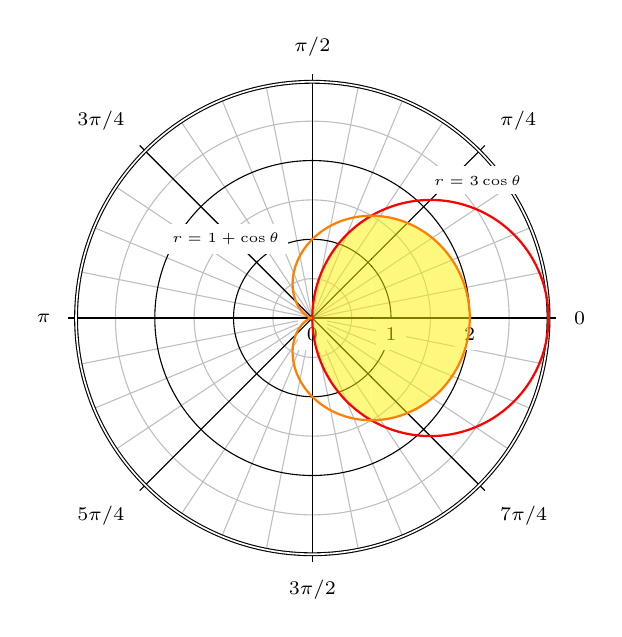
\begin{tikzpicture}
% Draw the lines at multiples of pi/12
\foreach \ang in {0,...,31} {
  \draw [lightgray] (0,0) -- (\ang * 180 / 16:3);
}

% Concentric circles and radius labels
\foreach \s in {0, 1, 2} {
  \draw [lightgray] (0,0) circle (\s + 0.5);
  \draw (0,0) circle (\s);
  \node [fill=white] at (\s, 0) [below] {\scriptsize $\s$};
}

% Add the labels at multiples of pi/4
\foreach \ang/\lab/\dir in {
  0/0/right,
  1/{\pi/4}/{above right},
  2/{\pi/2}/above,
  3/{3\pi/4}/{above left},
  4/{\pi}/left,
  5/{5\pi/4}/{below left},
  7/{7\pi/4}/{below right},
  6/{3\pi/2}/below} {
  \draw (0,0) -- (\ang * 180 / 4:3.1);
  \node [fill=white] at (\ang * 180 / 4:3.2) [\dir] {\scriptsize $\lab$};
}

% The double-lined circle around the whole diagram
\draw [style=double] (0,0) circle (3);

\fill [fill=yellow, opacity=0.5, samples=200] plot [domain=pi/3:2*pi/3]
	(xy polar cs:angle=\x r, radius= {3*cos(\x r)});
\draw [thick, color=red, domain=0:2*pi, samples=200, smooth]
	plot (xy polar cs:angle=\x r, radius={3*cos(\x r)});
\fill [fill=yellow, opacity=0.5, samples=200] plot [domain=-pi/3:pi/3]
	(xy polar cs:angle=\x r, radius= {1+cos(\x r)});
\draw [thick, color=orange, domain=0:2*pi, samples=200, smooth]
	plot (xy polar cs:angle=\x r, radius={1+cos(\x r)});
\node [fill=white] at (2.1,1.75) {\tiny $r=3\cos \theta$};
\node [fill=white] at (-1.1,1) {\tiny $r=1+\cos \theta$};
\end{tikzpicture}
\end{center}
\par 注意在实际解题过程中,并没有图画作为辅助,因此需要自己判断积分区间.
\par 首先求定义域.
\[r\geq 0 \implies \theta\in[-\dfrac{\pi}{2},\dfrac{\pi}{2}]\]
\par 其次求出两曲线交点.
\[r=1+\cos\theta=3\cos\theta\implies\theta=\pm\dfrac{\pi}{3}\]
\par 判断对称性.
由于$\cos\theta$为偶函数,故两曲线都关于极轴对称.
\par 考虑内外关系,对小极径所在曲线进行积分.
\[A=2\cdot\dfrac{1}{2}\lrp{\intabu{0}{\frac{\pi}{3}}{(1+\cos\theta)^2}{\theta}+\intabu{\frac{\pi}{3}}{\frac{\pi}{2}}{(3\cos\theta)^2}{\theta}}=\dfrac{5}{4}\pi\]
\end{analysis}
\par 如果是单一极坐标曲线求面积,则一般关注其最大最小极径以及其对称性.

\subsection{体积}
\begin{enumerate}
	\item 旋转体(不是绕$x$轴、$y$轴旋转,则先做一个平移)
\[\diff V=\pi[f(x)]^2\diff x\]
	\item 已知截面积
\[\diff V=A(x)\diff x\]
\end{enumerate}

\subsection{弧长}
\begin{center}
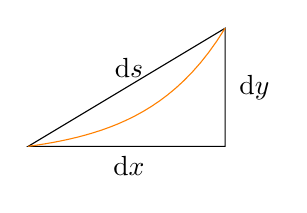
\begin{tikzpicture}[domain=0:2.5]
\draw (0,0) --node[below] {$\diff x$} (2.5,0) --node[right] {$\diff y$} (2.5,1.5) --node[left,above] {$\diff s$} cycle;
\draw[color=orange] plot (\x,{1.5/(exp(2.5)-1)*(exp(\x)-1)});
\end{tikzpicture}
\end{center}
\[\diff s=\sqrt{\diff x^2+\diff y^2}=\sqrt{1+\lrp{\dfrac{\diff y}{\diff x}}^2}\diff x\]
\begin{enumerate}
	\item 直角坐标
	\[\diff s^2=(1+[f'(x)]^2)\diff x^2\]
	\item 参数方程
	\[\diff s^2=([x(t)]^2+[y(t)]^2)\diff t^2\]
	\item 极坐标(通过$x=r\cos\theta,y=r\sin\theta$转直角坐标推导)
	\[\diff s^2=r^2\diff\theta^2+\diff r^2\]
\end{enumerate}

\subsection{曲率}
\begin{definition}[曲率]
用切线夹角与弧长之比来衡量曲线的弯曲程度,即
\[K=\left|\dfrac{\diff\varphi}{\diff s}\right|\]
\end{definition}
\begin{enumerate}
	\item 直角坐标
	\[K=\dfrac{|y''|}{(1+y'^2)^\frac{3}{2}}\]
	\item 参数方程(由参方推其他两个)
	\[K=\dfrac{|y''x'-y'x''|}{(x'^2+y'^2)^\frac{3}{2}}\]
	\item 极坐标
	\[K=\dfrac{|r^2+2r'^2-rr''|}{(r^2+r'^2)^\frac{3}{2}}\]
\end{enumerate}

\subsection{表面积}
旋转体的表面积可以通过以下的微元公式得到
\[\diff S=2\pi y\diff s\]
\par 注意想清楚取多少部分进行旋转,如上式的$y$仅仅是坐标轴一侧的$y$.
\begin{example}
求椭圆$\dfrac{x^2}{a^2}+\dfrac{y^2}{b^2}=1$绕$x$轴旋转所得旋转体的表面积
\end{example}
% http://www.nabla.hr/CL-DefiniteIntAppl5.htm
\begin{analysis}
本题解题方法来源于\footnote{Math StackExchange - How to Find the Surface Area of Revolution of An Ellipsoid from Ellipse Rotating, \url{https://math.stackexchange.com/questions/1379341}}.
对椭圆隐函数求导得
\[\frac{2x\diff x}{a^2} + \frac{2y\diff y}{b^2} = 0\]
故
\[\diff s = \sqrt{1 + (\frac{\diff y}{\diff x})^2}\diff x = \frac{1}{a^2}\,\frac{\diff x}{y}\,\sqrt{b^4x^2 + a^4y^2}\]
进而
\[\diff S = 2\pi y\diff s=2\pi \frac{1}{a^2}\,\sqrt{b^4x^2 + a^4y^2}\diff x\]
两边进行积分有
\[S = 2\frac{2\pi}{a^2}\int_{0}^{a} \sqrt{b^4x^2 + a^4y^2}\diff x\]
将
\[y^2 = b^2 - \frac{b^2}{a^2}\,x^2\]
代入有
\[S = 4\pi\,\frac{b}{a}\int_{0}^{a} \sqrt{a^2 - \varepsilon^2x^2}\diff x\]
其中,$\varepsilon^2=\sqrt{a^2-b^2}\Big/a^2$为椭圆离心率的平方,参数方程$x=a\sin\theta$
\[S = 4\pi\,ab\,\int_{0}^{\frac{\pi}{2}} \sqrt{1 - \varepsilon^2\sin^2\theta}\,\cos\theta\diff\theta\]
三角代换,令$\sin\phi = \varepsilon\sin\theta$,则$\cos\phi\diff\phi = \varepsilon\cos\theta\diff\theta$,故
\[S = 4\pi\,\frac{ab}{\varepsilon}\,\int\cos^2\phi\diff\phi\]
直接对其积分即可,将结果逐步回代得
\[S = 
2\pi\,\frac{ab}{\varepsilon}\lrp{\arcsin(\varepsilon) + \varepsilon\,\frac{b}{a}}= 
2\pi\,b^2\lrp{1 + \frac{a}{b}\,\frac{\arcsin(\varepsilon)}{\varepsilon}}\]
\end{analysis}

\subsection{质心}
\begin{theorem}[古鲁金(Guldin)第一定理]
质量分布均匀的平面曲线弧的质心坐标$(\bar{x},\bar{y})$由下式得出
\[2\pi\bar{x}l=S_1\qquad 2\pi\bar{y}l=S_2\]
其中,$S_1$和$S_2$分别为曲线弧绕$y$轴和绕$x$轴所得旋转体的侧面积,$l$为弧长.
\end{theorem}
其基本思想即将旋转体的侧面积转化为圆柱的侧面积.
\begin{theorem}[古鲁金第二定理]
质量分布均匀的平面图形绕此平面上一条与之不相交的直线旋转,所得旋转体的体积由下式给出
\[V=2\pi\bar{y}S\]
\end{theorem}

\subsection{切线与法线}
\subsubsection{空间曲线的切线与法平面}
曲线上一点$(x,y,z)$的切向量为
\[\mathbf{\tau}(x,y,z)=\pm(x'(t_0),y'(t_0),z'(t_0))=\pm\lrp{\pd{(F,G)}{(y,z)},\pd{(F,G)}{(z,x)},\pd{(F,G)}{(x,y)}}\]
若曲线在$P(x_0,y_0,z_0)$的切向量为
\[\mathbf{\tau}(x_0,y_0,z_0)=(A,B,C)\]
则该点的切线方程为
\[\frac{x-x_0}{A}=\frac{y-y_0}{B}=\frac{z-z_0}{C}\]
法平面方程为
\[\mathbf{\tau}\cdot(\vv-P)^\T=0\]

\subsubsection{空间曲面的切平面与法线}
法向量为
\[\mathbf{n}(x,y,z)=\pm(F_x,F_y,F_z)=\pm\lrp{\pd{(y,z)}{(u,v)},\pd{(z,x)}{(u,v)},\pd{(x,y)}{(u,v)}}\]
若曲线在$P(x_0,y_0,z_0)$的切向量为
\[\mathbf{n}(x_0,y_0,z_0)=(A',B',C')\]
则该点的法线方程为
\[\frac{x-x_0}{A'}=\frac{y-y_0}{B'}=\frac{z-z_0}{C'}\]
切平面方程为
\[\mathbf{n}\cdot(\vv-P)^\T=0\]

\subsubsection{方向导数}
即在某一个方向$\mathbf{l}$上的变化率
\begin{theorem}
若$f(x,y,z)$在点$P_0(x_0,y_0,z_0)$可微,则$f(x,y,z)$在$P_0$沿任何方向$\mathbf{l}$的方向导数都存在,且有
\[\pd{f(P_0)}{l}=\pd{f(P_0)}{x}\cos\alpha+\pd{f(P_0)}{y}\cos\beta+\pd{f(P_0)}{z}\cos\gamma=\nabla f(P_0)\cdot\cos\theta\]
其中,$\cos\alpha,\cos\beta,\cos\gamma$是$\mathbf{l}$的方向余弦,即$\mathbf{l}$与三个坐标轴的夹角
\end{theorem}

\end{document}